In addition to the three signal physics processes, parton initiated $qqZZ$, gluon-loop initiated $ggZZ$ and EWK $qqZZjj$, background processes such as $ttV$, $VVV$ and fake background comprising of \textit{non-prompt} leptons also contribute to the $ZZ(\rightarrow 4\ell) jj$ final state. As discussed in Section \ref{subsec:MCSamples}, the events originating from $ttV$ and $VVV$ processes are simulated using MC generators and subtracted from data.

\subsection{Data Driven Estimate of Fake Background}
\label{subsec:FakeBackground}

\textit{Non-prompt leptons} originate from a non-hard scatter source, either from a secondary interaction such as jet decay or from charged tracks misidentification. Figure \ref{fig:NonPromptLepton} shows an example of non-prompt lepton production. The hard scatter process produces a b-jet which in secondary interaction produces a muon whose track does not point towards the interaction vertex and is surrounded by jet activities. The signal lepton criteria of isolation and TTVA discussed in Section \ref{sec:ObjReconstruction} discards most of the non-prompt leptons. However, some non-prompt leptons pass the signal criteria and, in association with other prompt leptons, form a quadruplet in the signal region. Thus, giving rise to the \textit{fake background} or \textit{non-prompt background} events for the analysis. The origins of non-prompt leptons are discussed in detail in Section \ref{subsubsec:LepComp}.

\begin{figure}
    \centering
    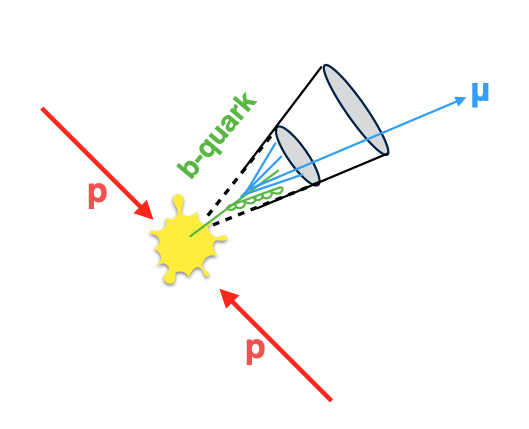
\includegraphics[width=.7\linewidth]{figures/Analysis/Background/NonPromptLeptonExample.png}  
    \caption{A schematic of the non-prompt lepton from semi-leptonic decays of b-hadrons. Jet activities surround the non-prompt muon, and the muon track does not point to the hard scatter interaction point.\label{fig:NonPromptLepton}}
\end{figure}

The fake backgrounds could be predicted using the MC for $Z(\rightarrow \ell \ell) + jets $, $t\bar{t}$ and $WZ$ processes where one or more non-prompt leptons in association with the prompt leptons form a signal quadruplet. However, it is difficult to predict the statistically limited contribution of fake backgrounds precisely using MC generators. It is also challenging to precisely model the non-prompt leptons originating from the reconstruction effects. Therefore, the fake backgrounds are estimated using an entirely data-driven technique discussed in this Section. Figure \ref{fig:FakeBkgOverview} shows the schematic of the whole background estimation process. The fake factors are evaluated from a combined control region (CR), formed by combining two independent control regions $Z+jets$ and $t\bar{t}$. Both regions are enriched in non-prompt leptons, and the combination is discussed in Section \ref{subsubsec:CR}. Section \ref{subsubsec:EstimationStrategy} discusses the technical aspects of the fake factor method, and Section \ref{subsubsec:FakeEff} discusses the fake efficiencies. The fake background is estimated by applying the fake factors to each anti-signal lepton in not-signal quadruplets. First, the background estimation technique is validated in fake-enriched validation regions discussed in Section \ref{subsubsec:Validation} and applied to the signal region, which is discussed in Section \ref{subsubsec:SREstimation}. 

\begin{figure}
    \centering
    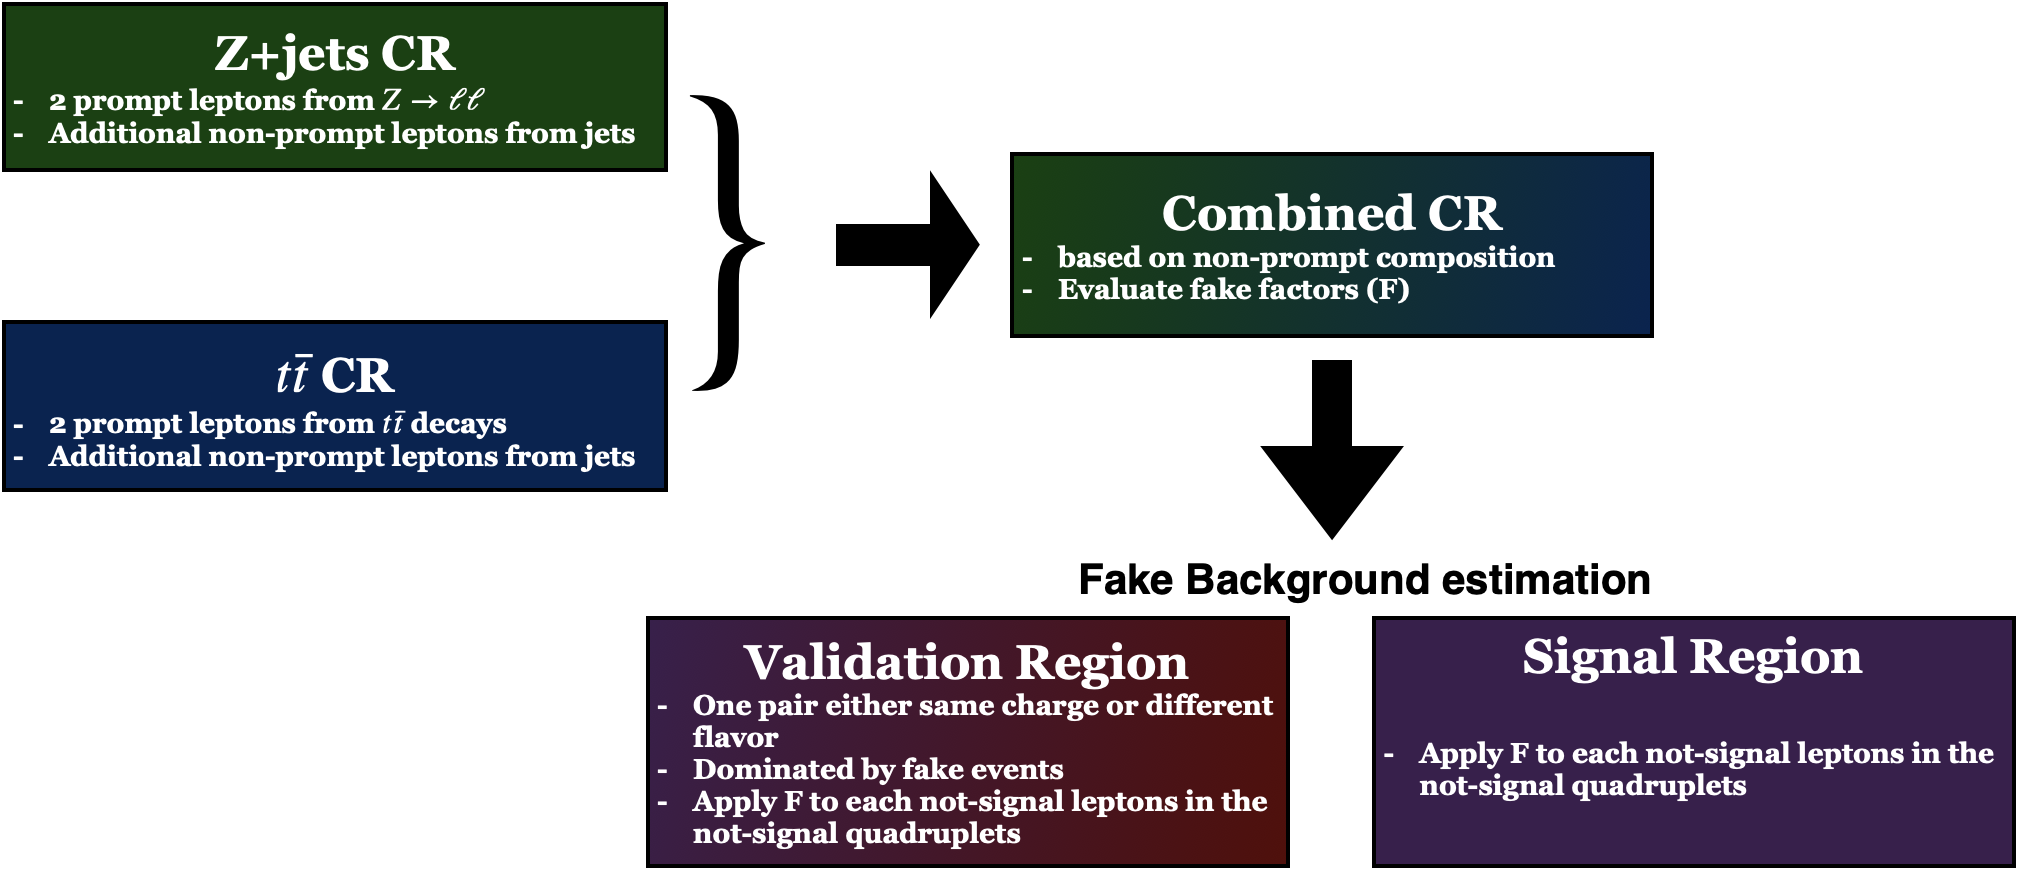
\includegraphics[width=.99\linewidth, angle =0]{figures/Analysis/Background/FakeBackgroundOverview.png}  
    \caption{An overview of the fake background estimation.\label{fig:FakeBkgOverview}}
\end{figure}

\subsubsection{Lepton Composition}
\label{subsubsec:LepComp}
The fake background MC predictions provide essential insight into the origin of the non-prompt leptons. A classification tool\footnote{https://gitlab.cern.ch/atlas/athena/-/tree/21.2/PhysicsAnalysis/AnalysisCommon/TruthClassification} developed by the ATLAS Isolation and Fake Forum (IFF) identifies the true origin of the leptons, which is studied to understand the composition of non-prompt leptons in various phase-space regions of the analysis. The tool has the following classification of truth origin for a non-prompt lepton

\begin{itemize}
    \item{ \textit{Unknown or KnownUnknown}: leptons with insufficient truth-level information to be classified by the tool.}
 
    \item { \textit{IsoElectron}: electrons originate either from the hard scatter or a boson decay. These electrons are treated as prompts in signal and background control regions.}
    
    \item{ \textit{ChargeFlipIsoElectron}: electrons whose charge is mismeasured at detector level and is classified as a non-prompt.}
    
    \item{ \textit{PromptMuon}: muons originate from either the hard scatter or a boson decay. These muons are treated as prompts for signal and background control regions.}
    
    \item{\textit{PromptPhotonConversion}: non-prompt electrons originating from photon conversion. }
    
    \item{\textit{TauDecay}: leptons originating from tau decays are treated as prompt leptons.}
    
    \item{\textit{BHadronDecay}: leptons originating from hadrons containing a b-quark. These types of leptons are one of the primary sources of non-prompt leptons.}
    
    \item{\textit{CHadronDecay}: leptons originating from hadrons containing a c-quark.}
    
    \item{\textit{LightFlavourDecay}: leptons originating from mesons and lighter hadrons.}

\end{itemize}

Figure \ref{fig:LeptonCompositionSRVBS} shows the origin of all leptons that are part of the quadruplet in the events with a signal quadruplet and a dijet. Most of the leptons in these regions are prompt and predominantly originate from $ggZZ$, $qqZZ$, and $ EWK qqZZjj$ processes. The leptons are classified \textit{Unknown/KnownUnknown} due to insufficient truth information and mainly originate from $ttZ(\rightarrow \ell \ell)$ and $VVV$ processes. Due to technical implementation in these simulations, it lacks information on the intermediary bosons for these samples, thus failing to identify the lepton origin. The \textit{Unknown/KnownUnknown} leptons are treated as prompt leptons in the signal region. This treatment relies on the fact that $\Delta R$ between the \textit{Unknown/KnownUnknown} classified truth leptons and reconstruction level lepton is observed to be close to $0$. The \textit{Unknown/KnownUnknown} classified leptons are treated as non-prompt leptons in the background control regions. 

Figure \ref{fig:NonPromptLepSRDijet} shows the predicted fraction of non-prompt electrons (left) and non-prompt muons (bottom) in the events with a signal quadruplet and a dijet. The non-prompt leptons originating from $b$-hadrons or $c$-hadrons are collectively called \textit{heavy flavor (HF)} non-prompt leptons, whereas all other non-prompt leptons are categorized as \textit{light flavor (LF)}. About $50\%$ of non-prompt electrons in the signal region originate from heavy flavor sources, whereas more than $90\%$ of non-prompt muons originate from the heavy flavor decays.

\begin{figure}[htb]
    \centering
    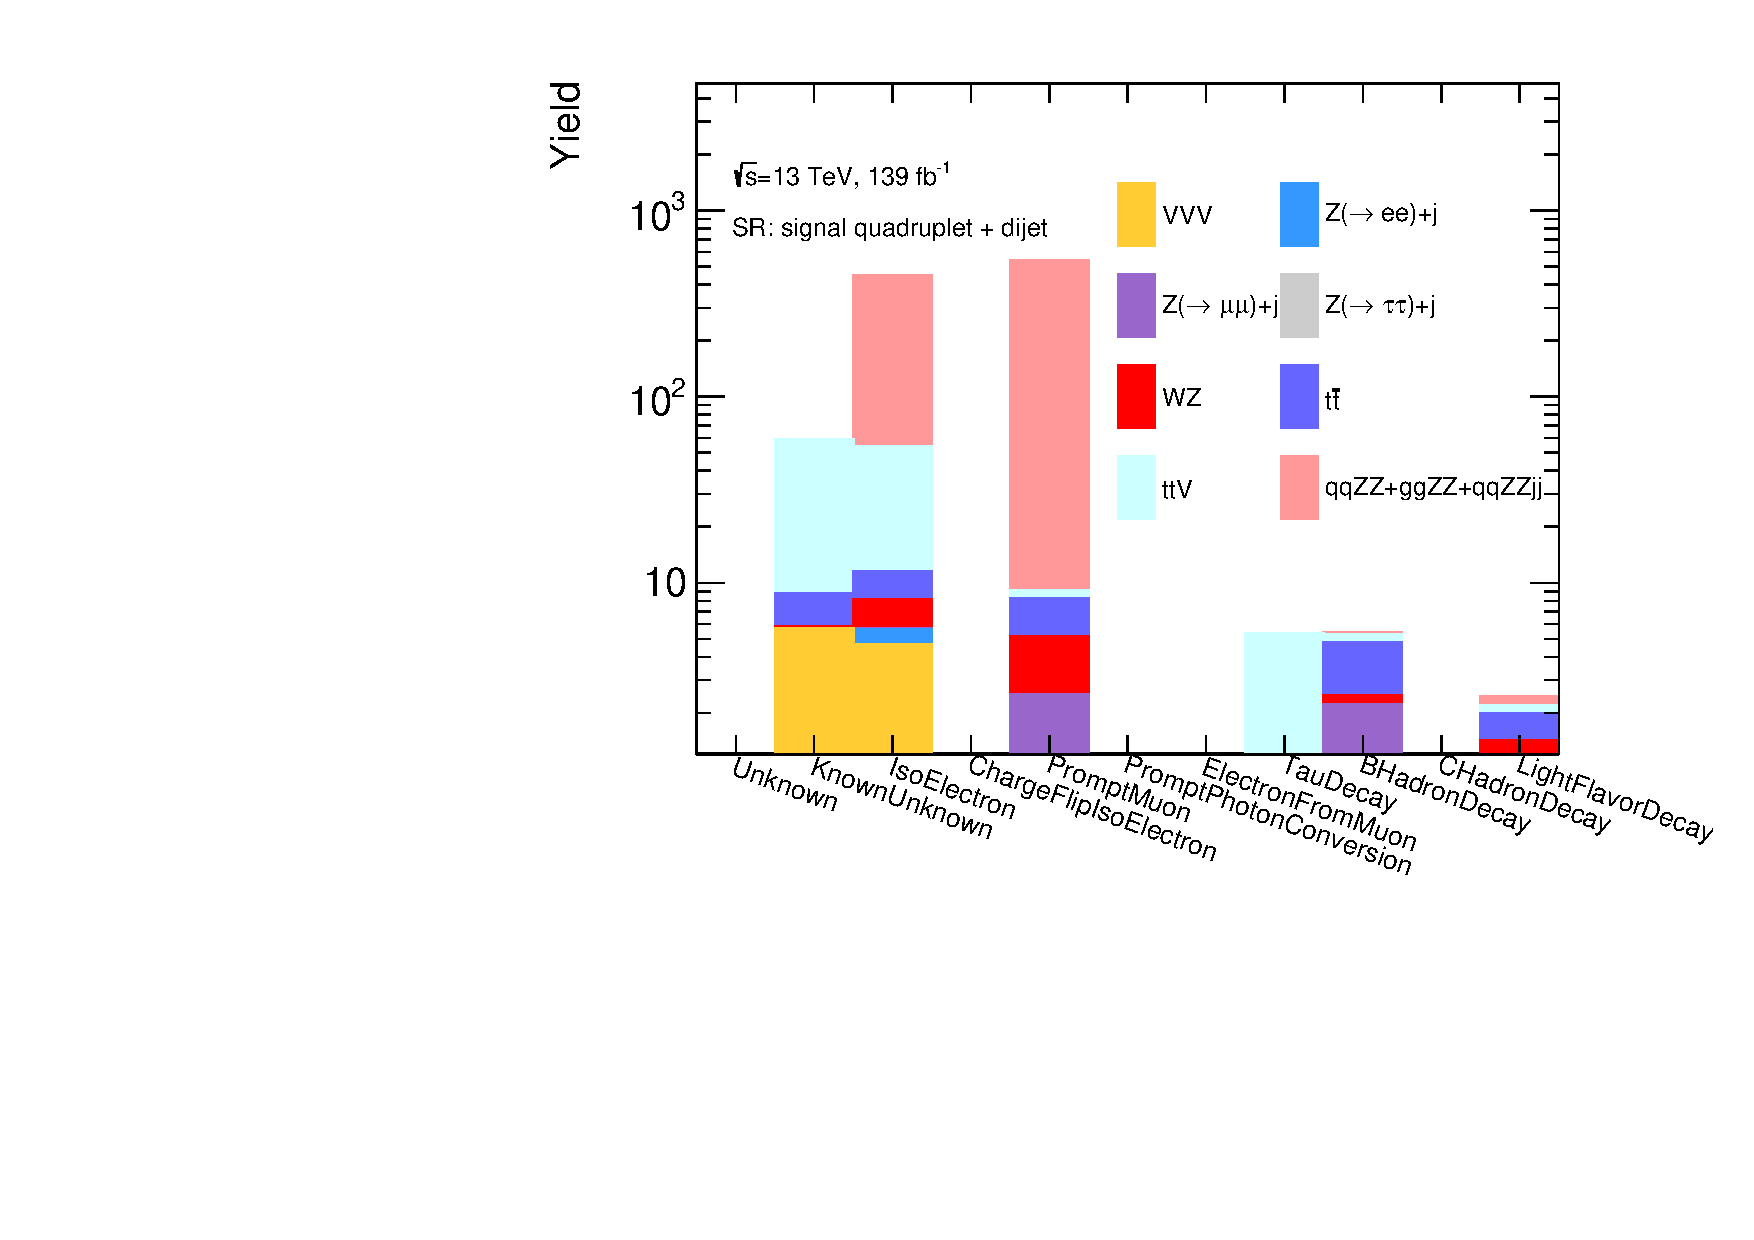
\includegraphics[width = 0.8\textwidth]{figures/Analysis/Background/AllLeptonSRDijetComposition.pdf}
    \caption{ Origins of leptons in the signal region in events with a quadruplet and a dijet. The lepton origin is classified by the IFF classifier tool. Only leptons that are part of the signal quadruplet are shown.\label{fig:LeptonCompositionSRVBS}}
\end{figure}

\begin{figure}[htb]
    \centering
    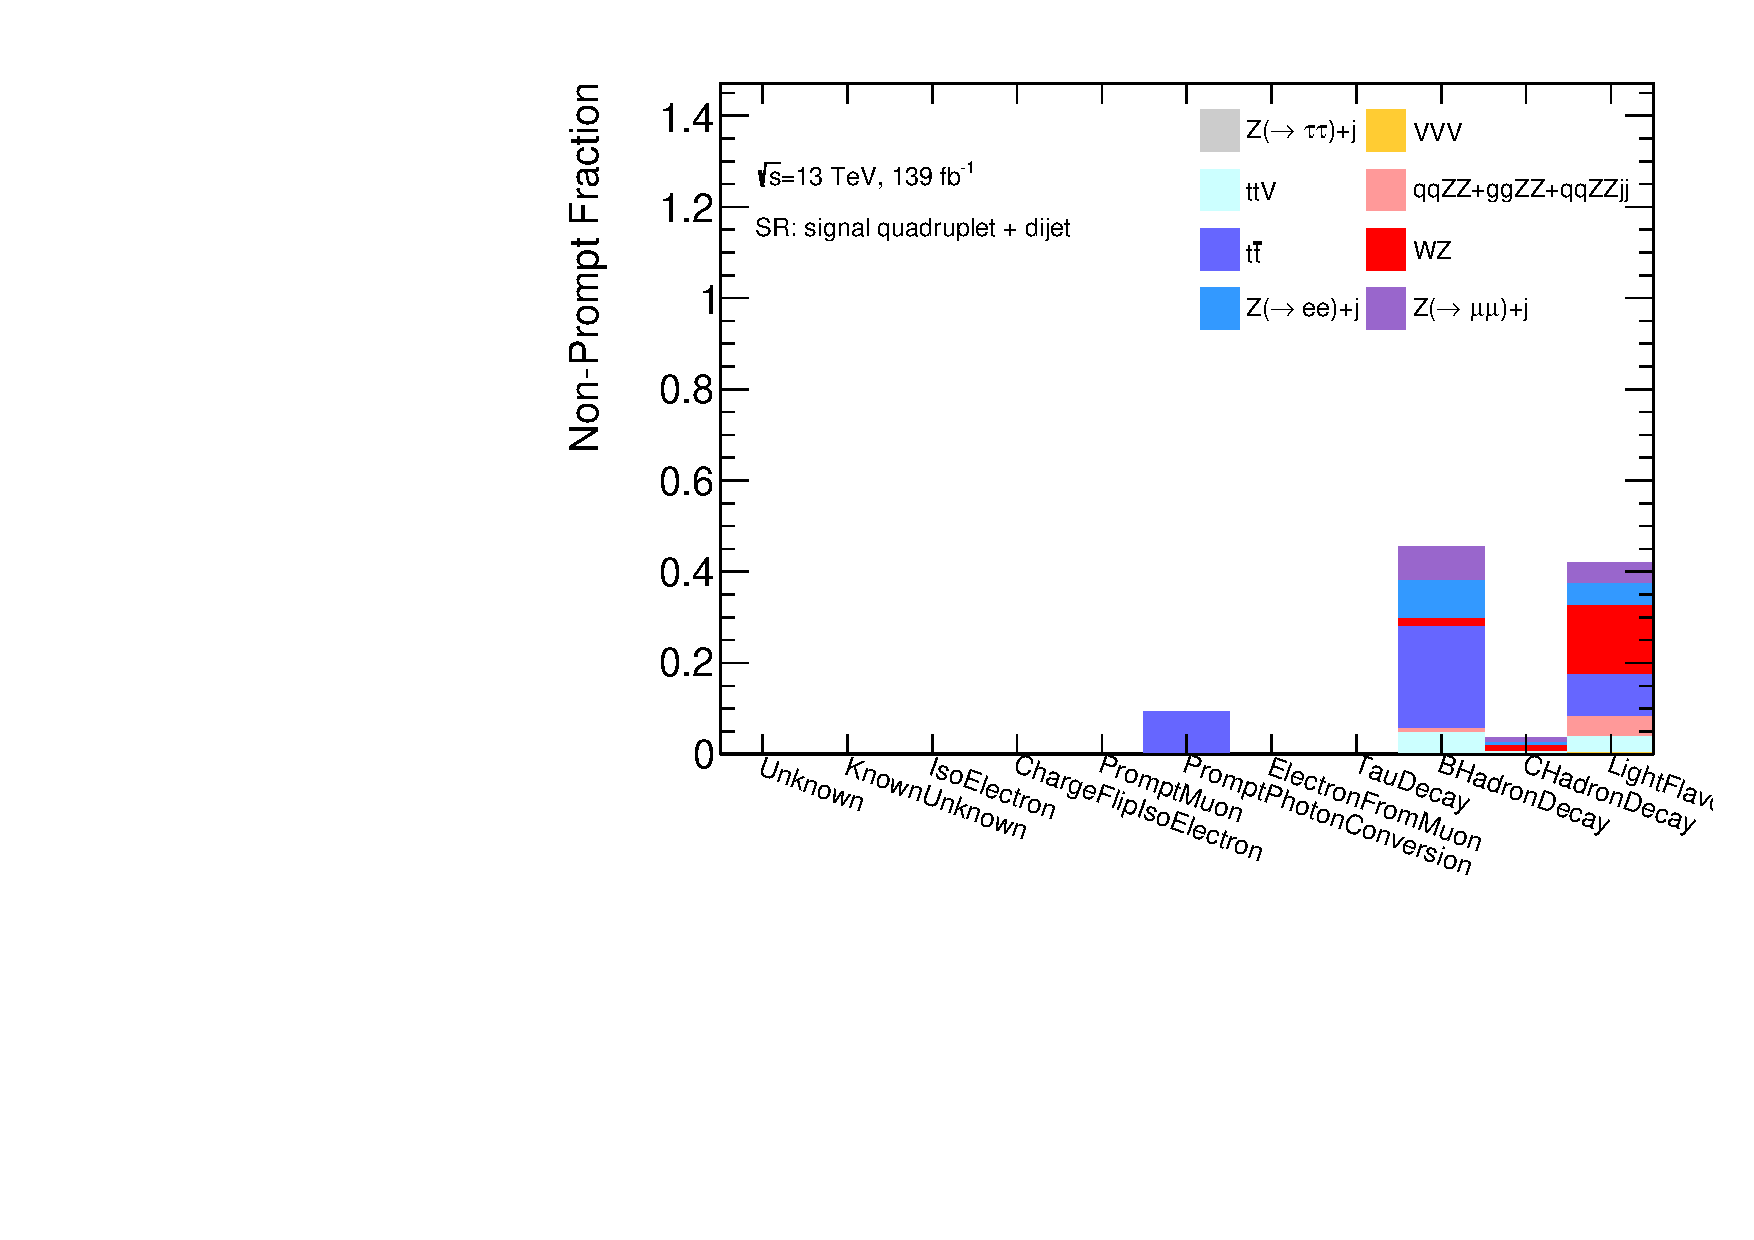
\includegraphics[width = 0.49\textwidth]{figures/Analysis/Background/NonPromptElectronSRVBSComposition.pdf}
    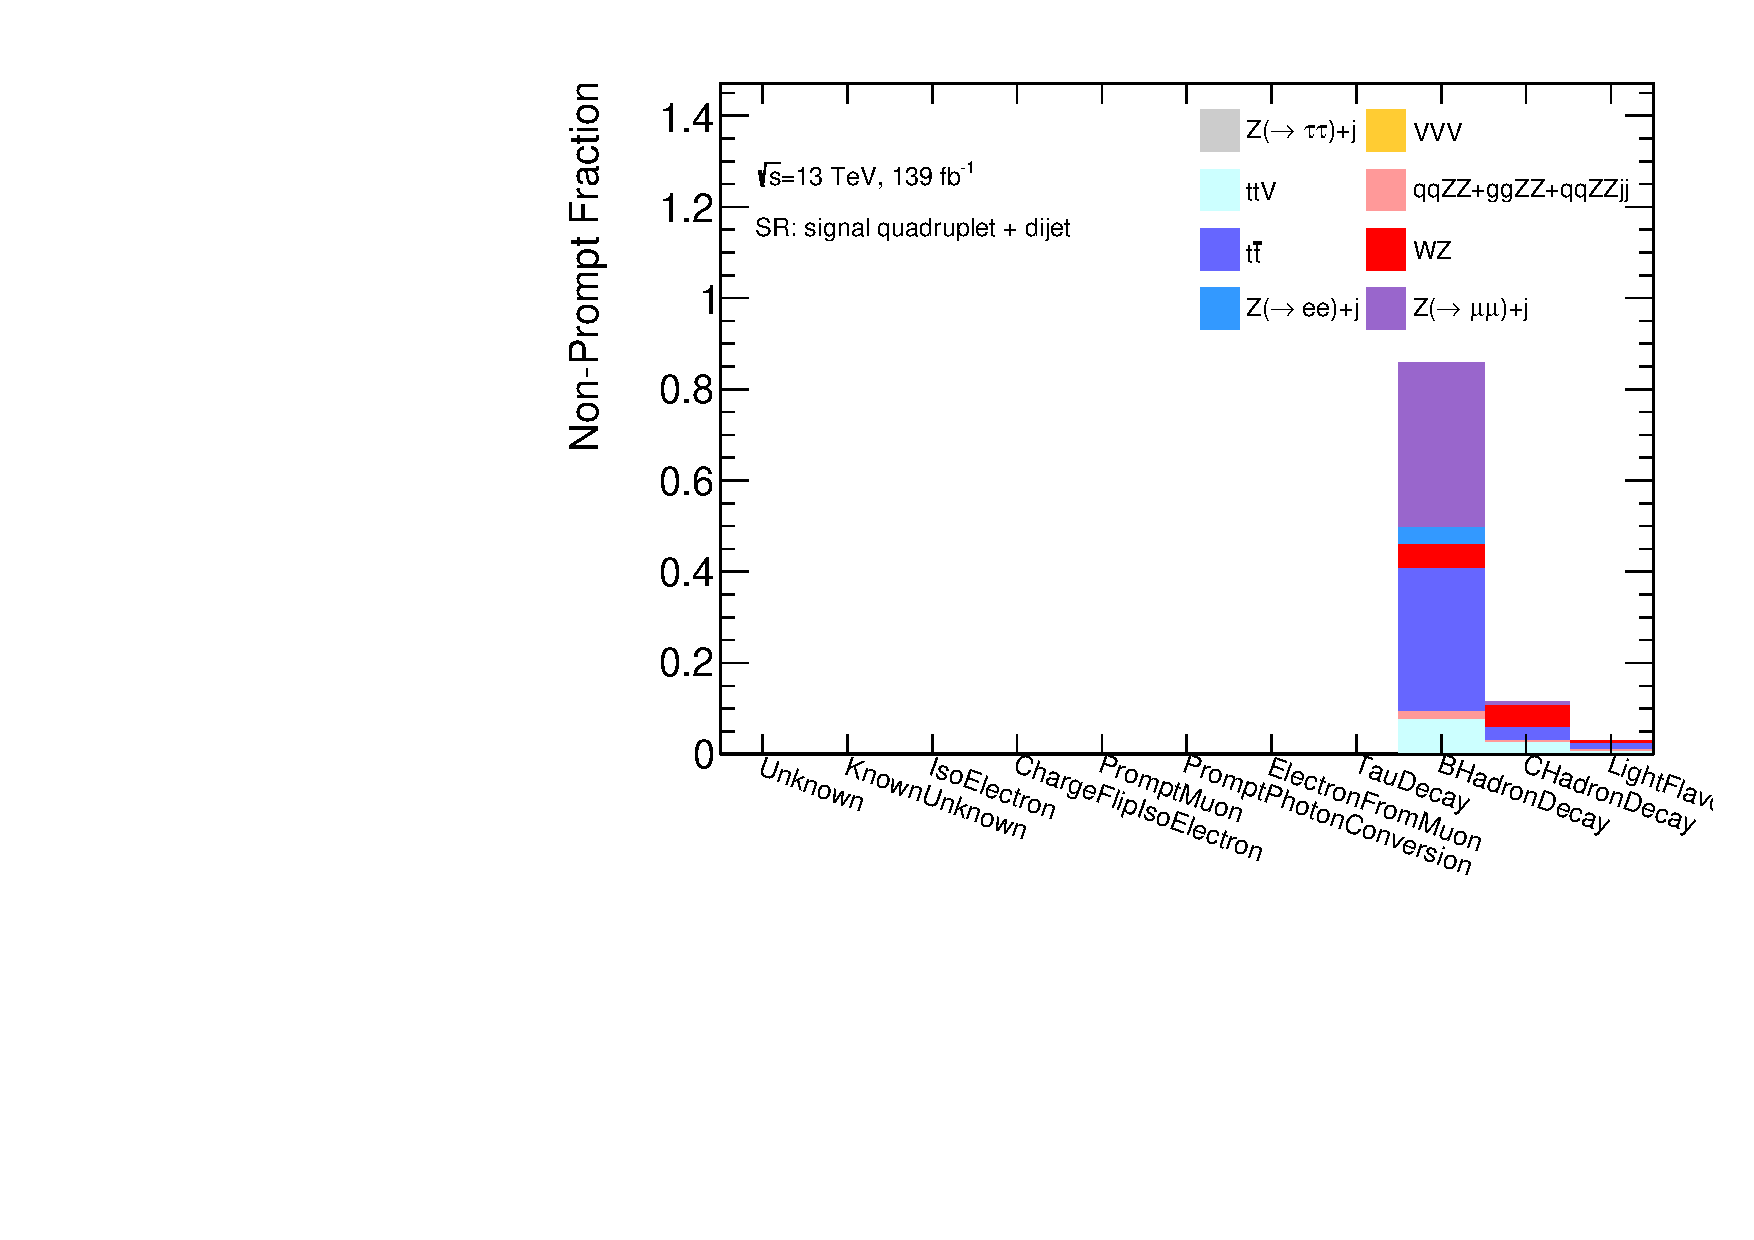
\includegraphics[width = 0.49\textwidth]{figures/Analysis/Background/NonPromptMuonSRVBSComposition.pdf}
    \caption{ Origins of non-prompt electrons (left) and muons (right) in the signal region in events with a signal quadruplet and a dijet. The events are normalized to the number of non-prompt electrons (left) and non-prompt muons (right). \label{fig:NonPromptLepSRDijet}}
\end{figure}

\subsubsection{Control Regions}
\label{subsubsec:CR}
The fake factors are measured from data in a fake enriched background control region formed by combining two independent control regions, the $Z+jets$ control region and the $t\bar{t}$ control region. An event in the control regions consists of a prompt lepton pair from a physics process and additional leptons from non-prompt sources. Both control regions use a single or di-lepton trigger similar to the signal region and require the leading and sub-leading leptons in an event to satisfy $p_{T,~leading~lepton} > 20$ GeV and $p_{T,~sub-leading~lepton} > 15$ GeV. An event in the $Z+jets$ CR consists of an SF-OC prompt-lepton pair from the Z boson decay with an invariant mass of $ 76~GeV~<~m_{\ell \ell}~<~106~GeV$, and additional leptons. Additionally, no events can have missing transverse energy higher than $50$ GeV to suppress the contamination from the $WZ$ process. Similarly, the $t\bar{t}$ CR consists of events with different flavor prompt-lepton pairs and additional leptons. An event in the $t\bar{t}$ CR requires at least one b-tagged jet to reduce the $WZ$ contamination. The b-tagging in the $t\bar{t}$ CR is performed by a flavor tagging tool described in Ref \cite{btagATLAS}.

Figure \ref{fig:FakeFractionBaseline} shows the fake fractions, fraction of leptons originating from a non-prompt source of the additional baseline electrons (left) and muons (right) as a function of their $p_{T}$ in the $Z+jets$ CR and the $t\bar{t}$ CR. A high fraction ($\geq 80\%$) of baseline electrons originate from non-prompt sources in both $Z+jets$ CR and $t\bar{t}$ CR. More than $95\%$ of the low-$p_{T}$ baseline muons are from non-prompt sources in both control regions. These distributions show that most of the additional leptons in either control region are expected to be from non-prompt sources, thus,  motivating the control regions to evaluate the fake factors.

\begin{figure}[htb]
    \begin{subfigure}{.48\textwidth}
        \centering
        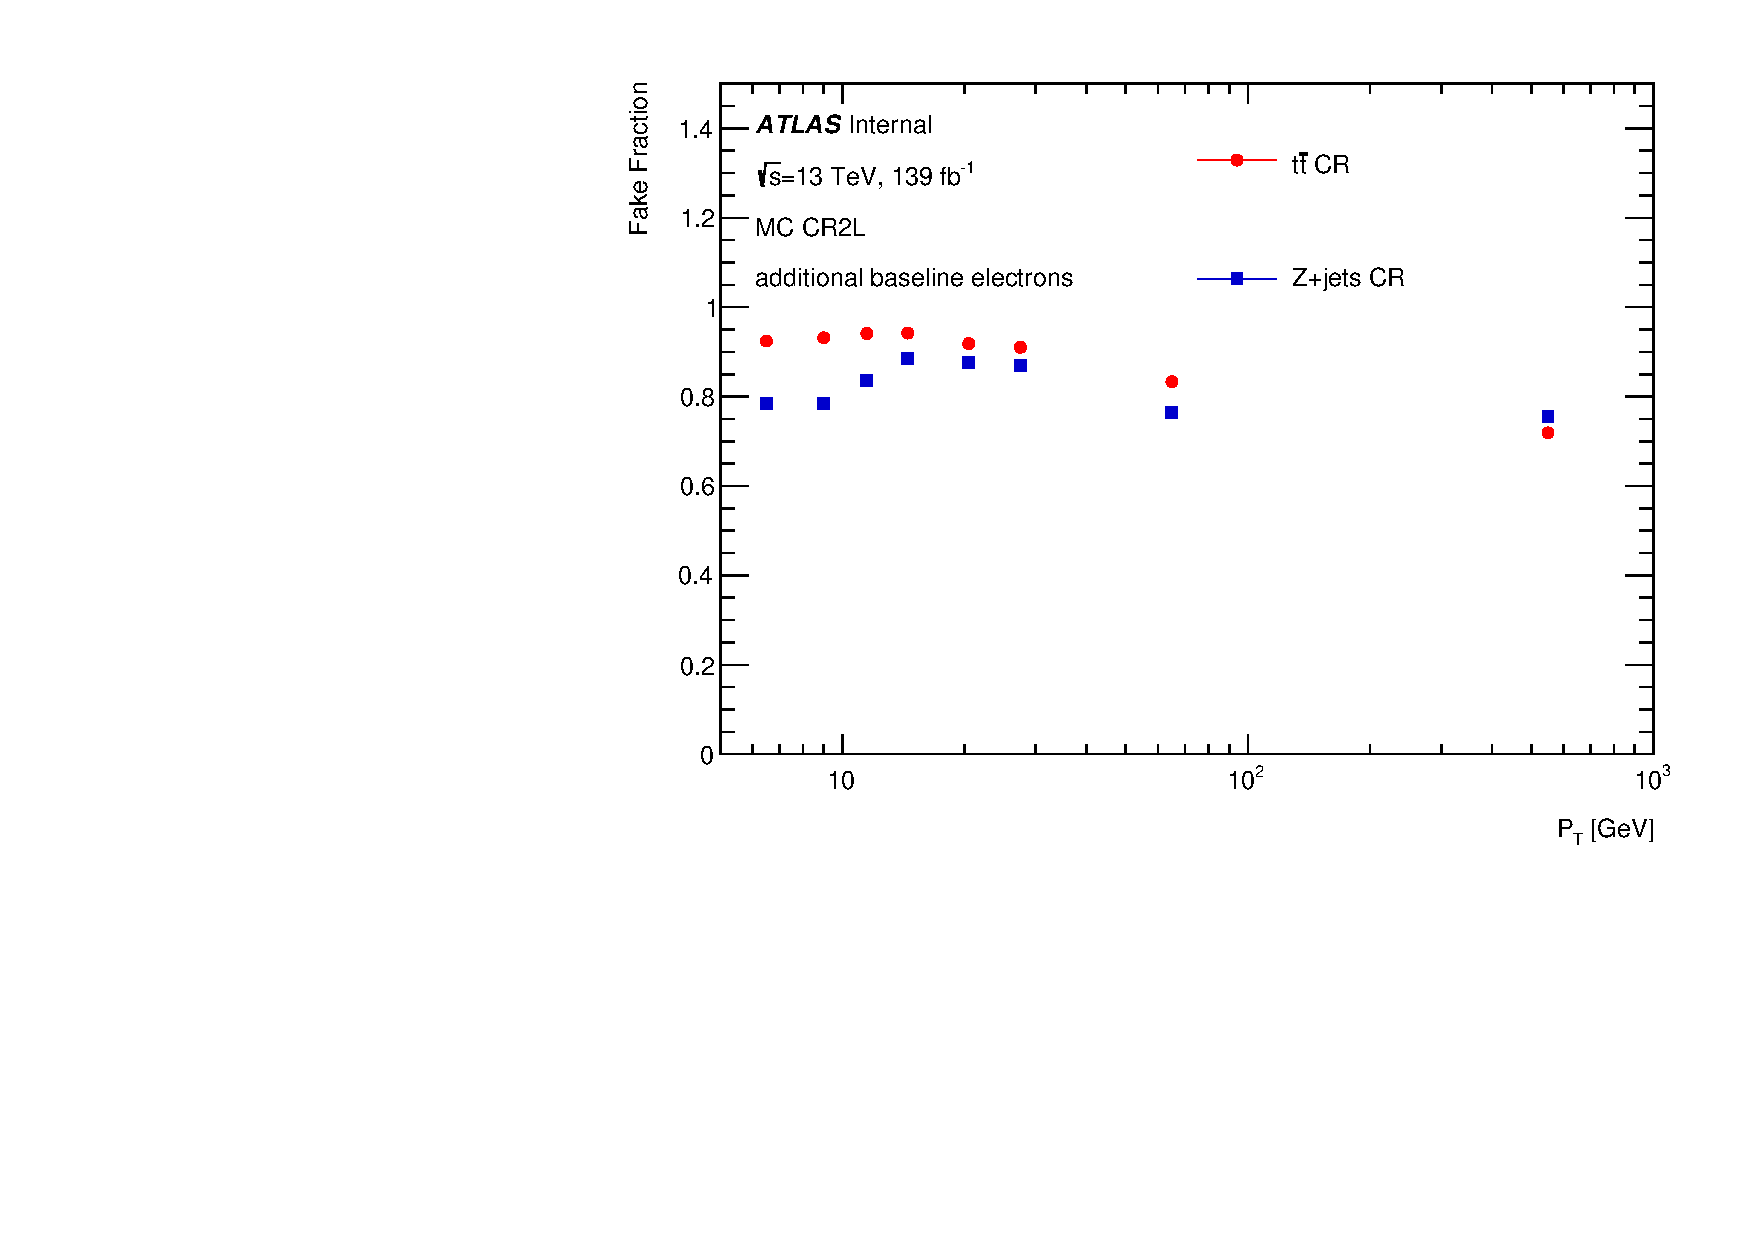
\includegraphics[width=.9\linewidth]{figures/Analysis/Background/FakeFractionBaselineElectrons.pdf}
        \caption{Fake-fraction of baseline electrons.}
    \end{subfigure}
    \begin{subfigure}{.48\textwidth}
        \centering
        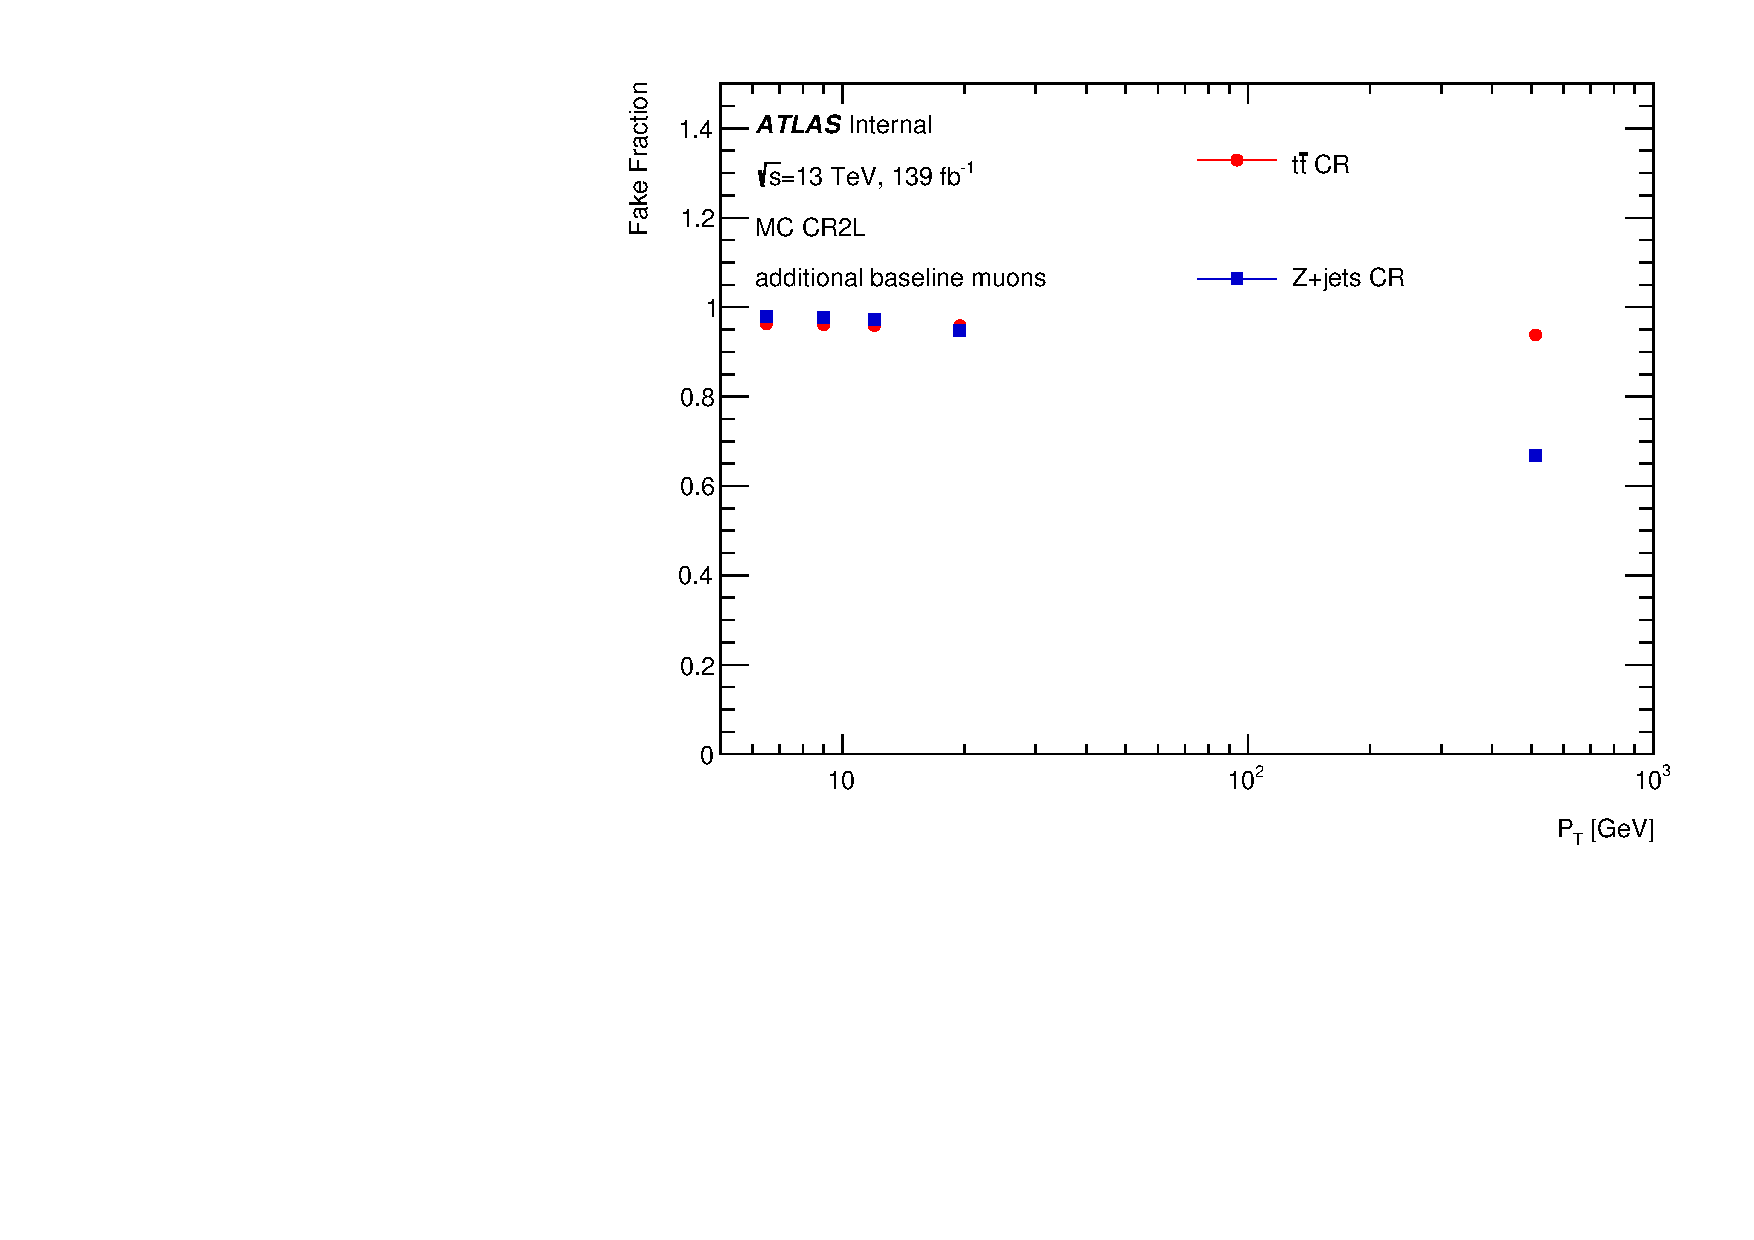
\includegraphics[width=.9\linewidth]{figures/Analysis/Background/FakeFractionBaselineMuons.pdf}
        \caption{Fake-fraction of baseline muons.}
    \end{subfigure}
        \caption{Fraction of non-prompt electrons and muons in the $Z+jets$ and $t\bar{t}$ control regions. \label{fig:FakeFractionBaseline}}
\end{figure}

The control regions have a unique non-prompt lepton composition as shown by Figures \ref{fig:FakeCompositionCR2LElectron} and \ref{fig:FakeCompositionCR2LMuon}. More than $80\%$ of the non-prompt electrons in the $Z+jets$ CR originate from the light flavor decays, but about $60\%$ are from the light flavor decays in the $t\bar{t}$ CR. Similarly, about $80\%$ of the non-prompt muons in the $Z+jets$ CR originate from the heavy flavor, whereas more than $90\%$ are from the heavy-flavor decays in the $t\bar{t}$ CR. The non-prompt compositions of the signal region shown in Figure \ref{fig:NonPromptLepSRDijet} are different from either control region. The two independent control regions are combined to form a single control region with a similar non-prompt lepton composition as the signal region.

\begin{figure}[ht]
    \begin{subfigure}{.48\textwidth}
      \centering
      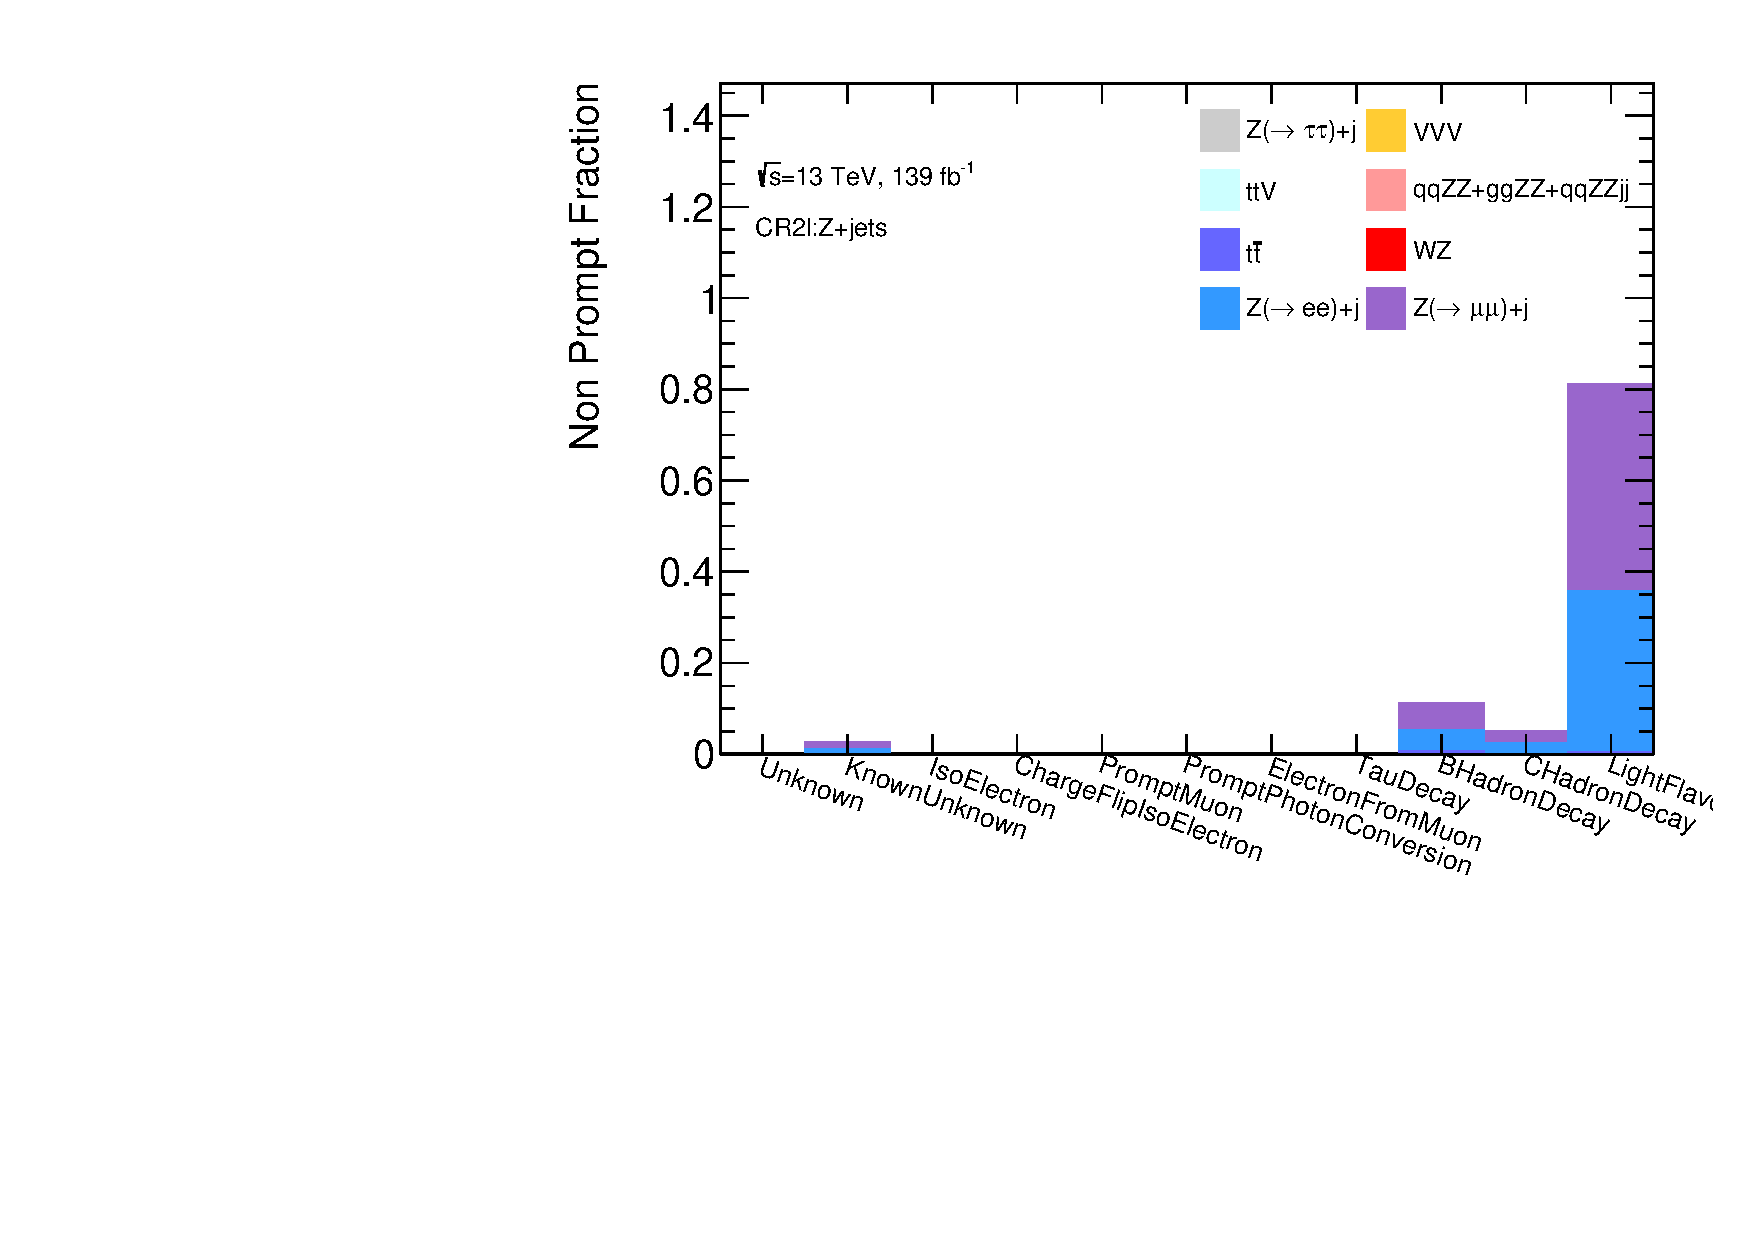
\includegraphics[width=.9\linewidth]{figures/Analysis/Background/NonPromptComposition_ZplusX_Electrons.pdf}  
      \caption{Non-prompt electrons in $Z+jets$ CR.}
    \end{subfigure}
    \begin{subfigure}{.48\textwidth}
      \centering
      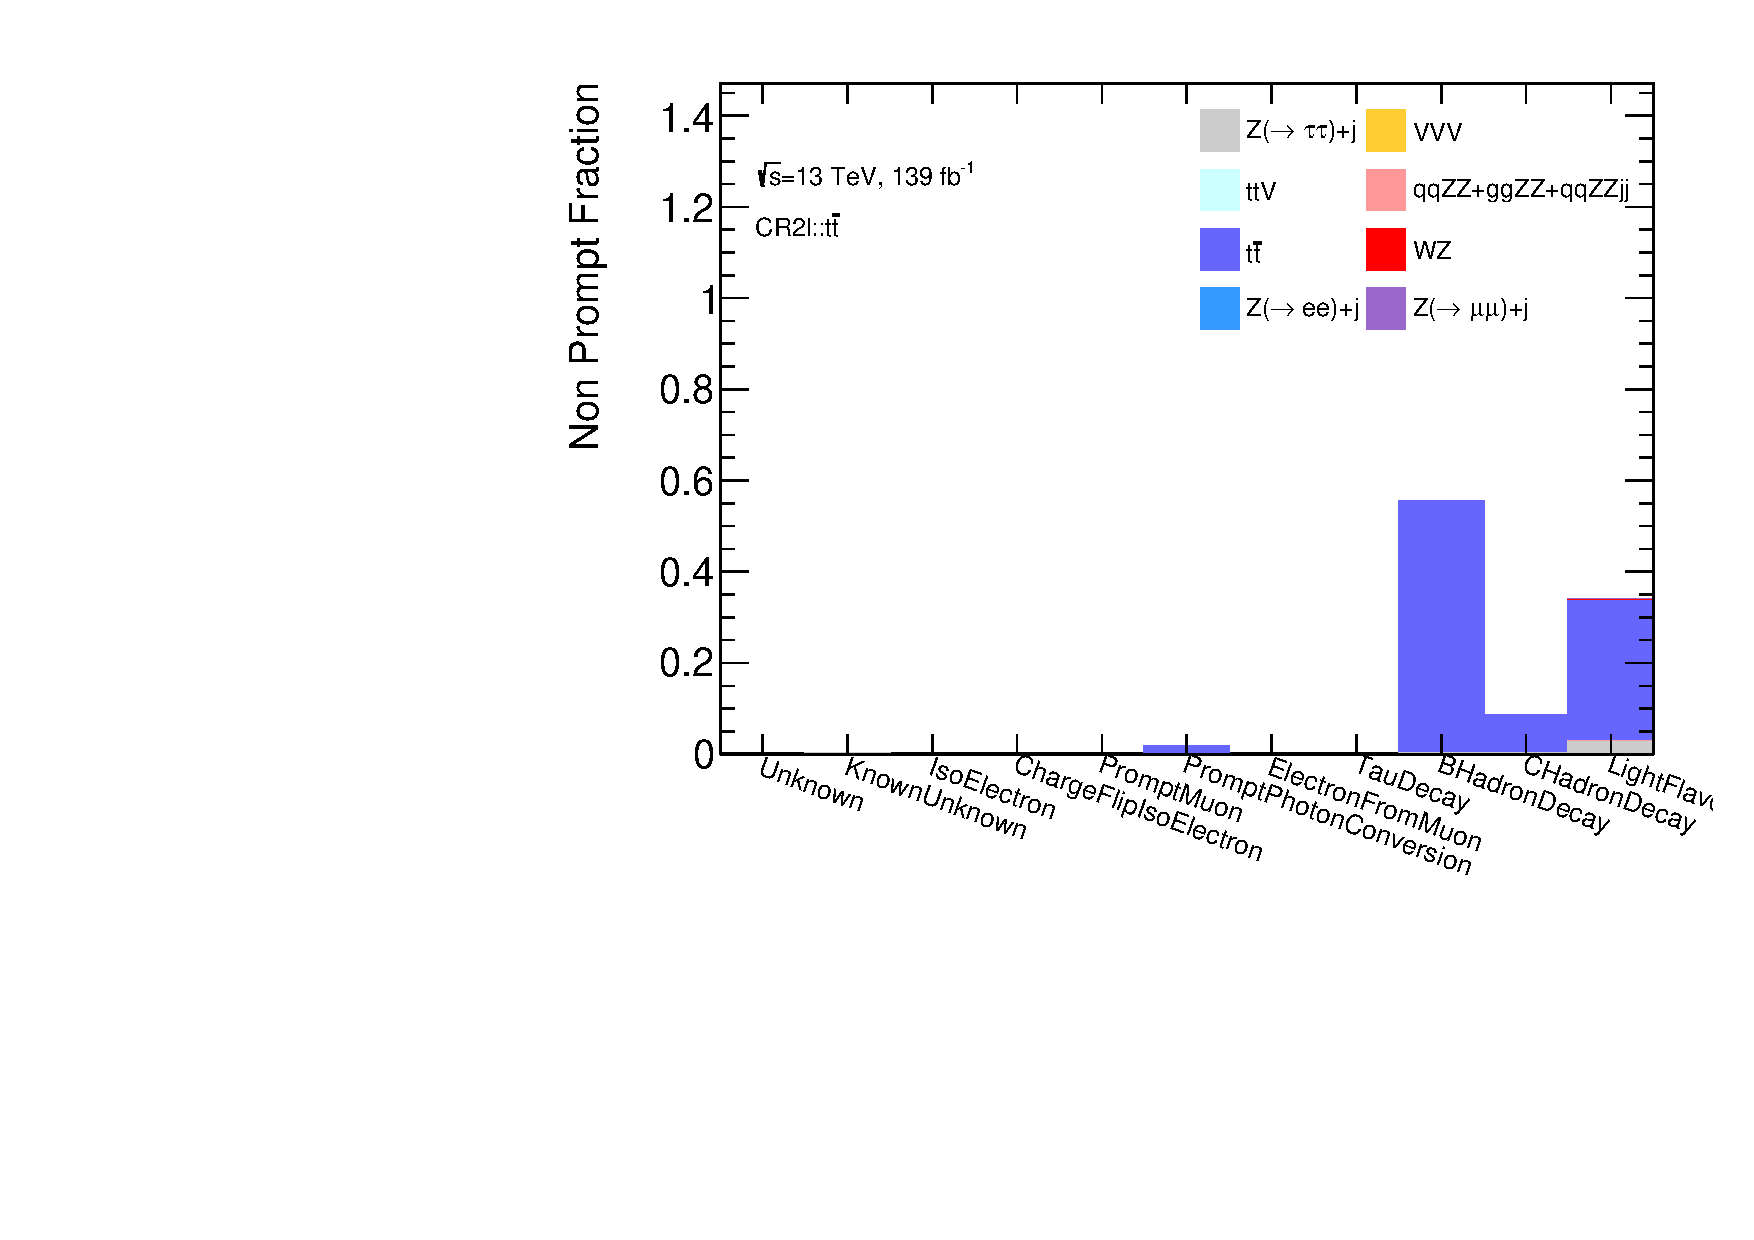
\includegraphics[width=.9\linewidth]{figures/Analysis/Background/NonPromptComposition_ttbar_Electrons.pdf}
      \caption{Non-prompt electrons in $t\bar{t}$ CR.}
    \end{subfigure}
    \caption{Sources of non-prompt electrons in background control regions. Fake composition is unique in these control regions.\label{fig:FakeCompositionCR2LElectron}}
    \end{figure}

\begin{figure}[htb]
    \begin{subfigure}{.48\textwidth}
        \centering
        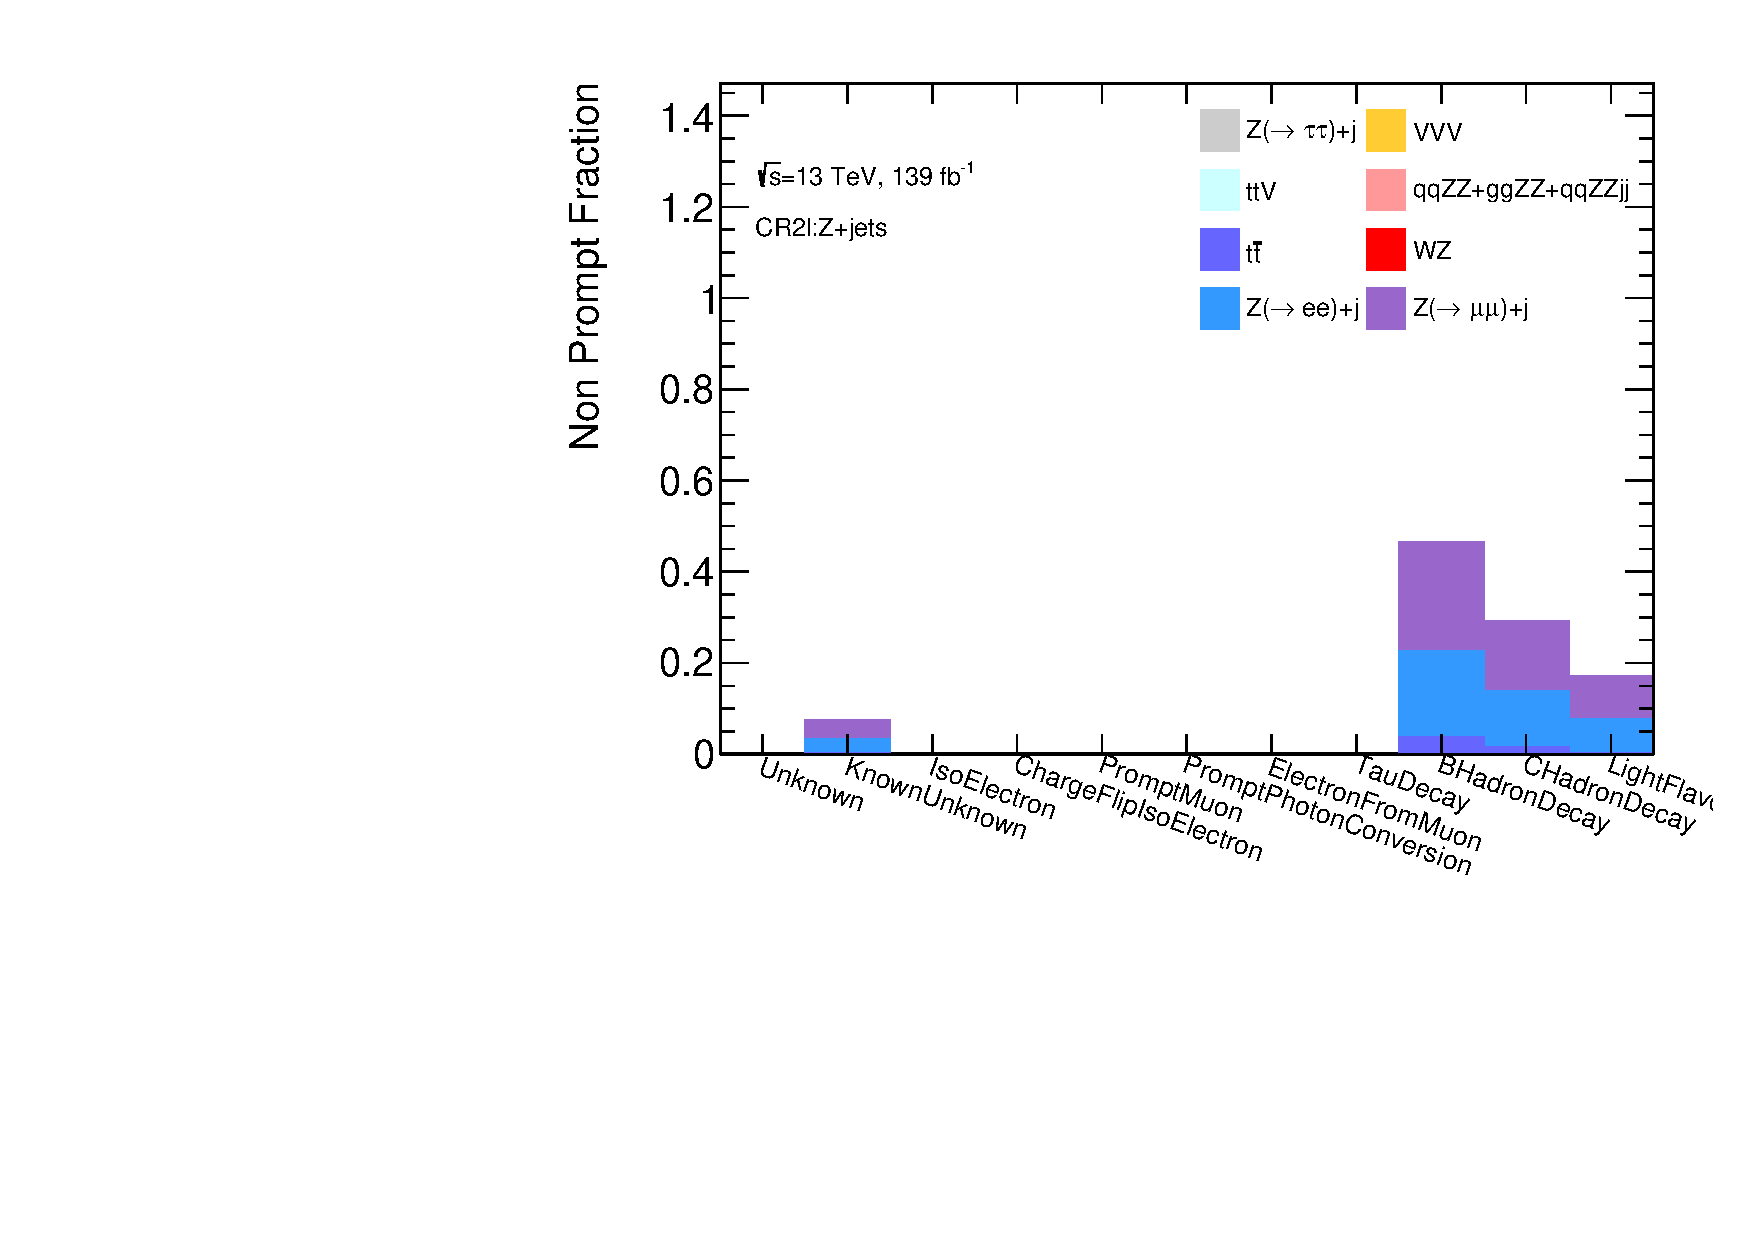
\includegraphics[width=.9\linewidth]{figures/Analysis/Background/NonPromptComposition_ZplusX_Muon.pdf}
        \caption{Non-prompt muons in $Z+jets$ CR.}
    \end{subfigure}
    \begin{subfigure}{.48\textwidth}
        \centering
        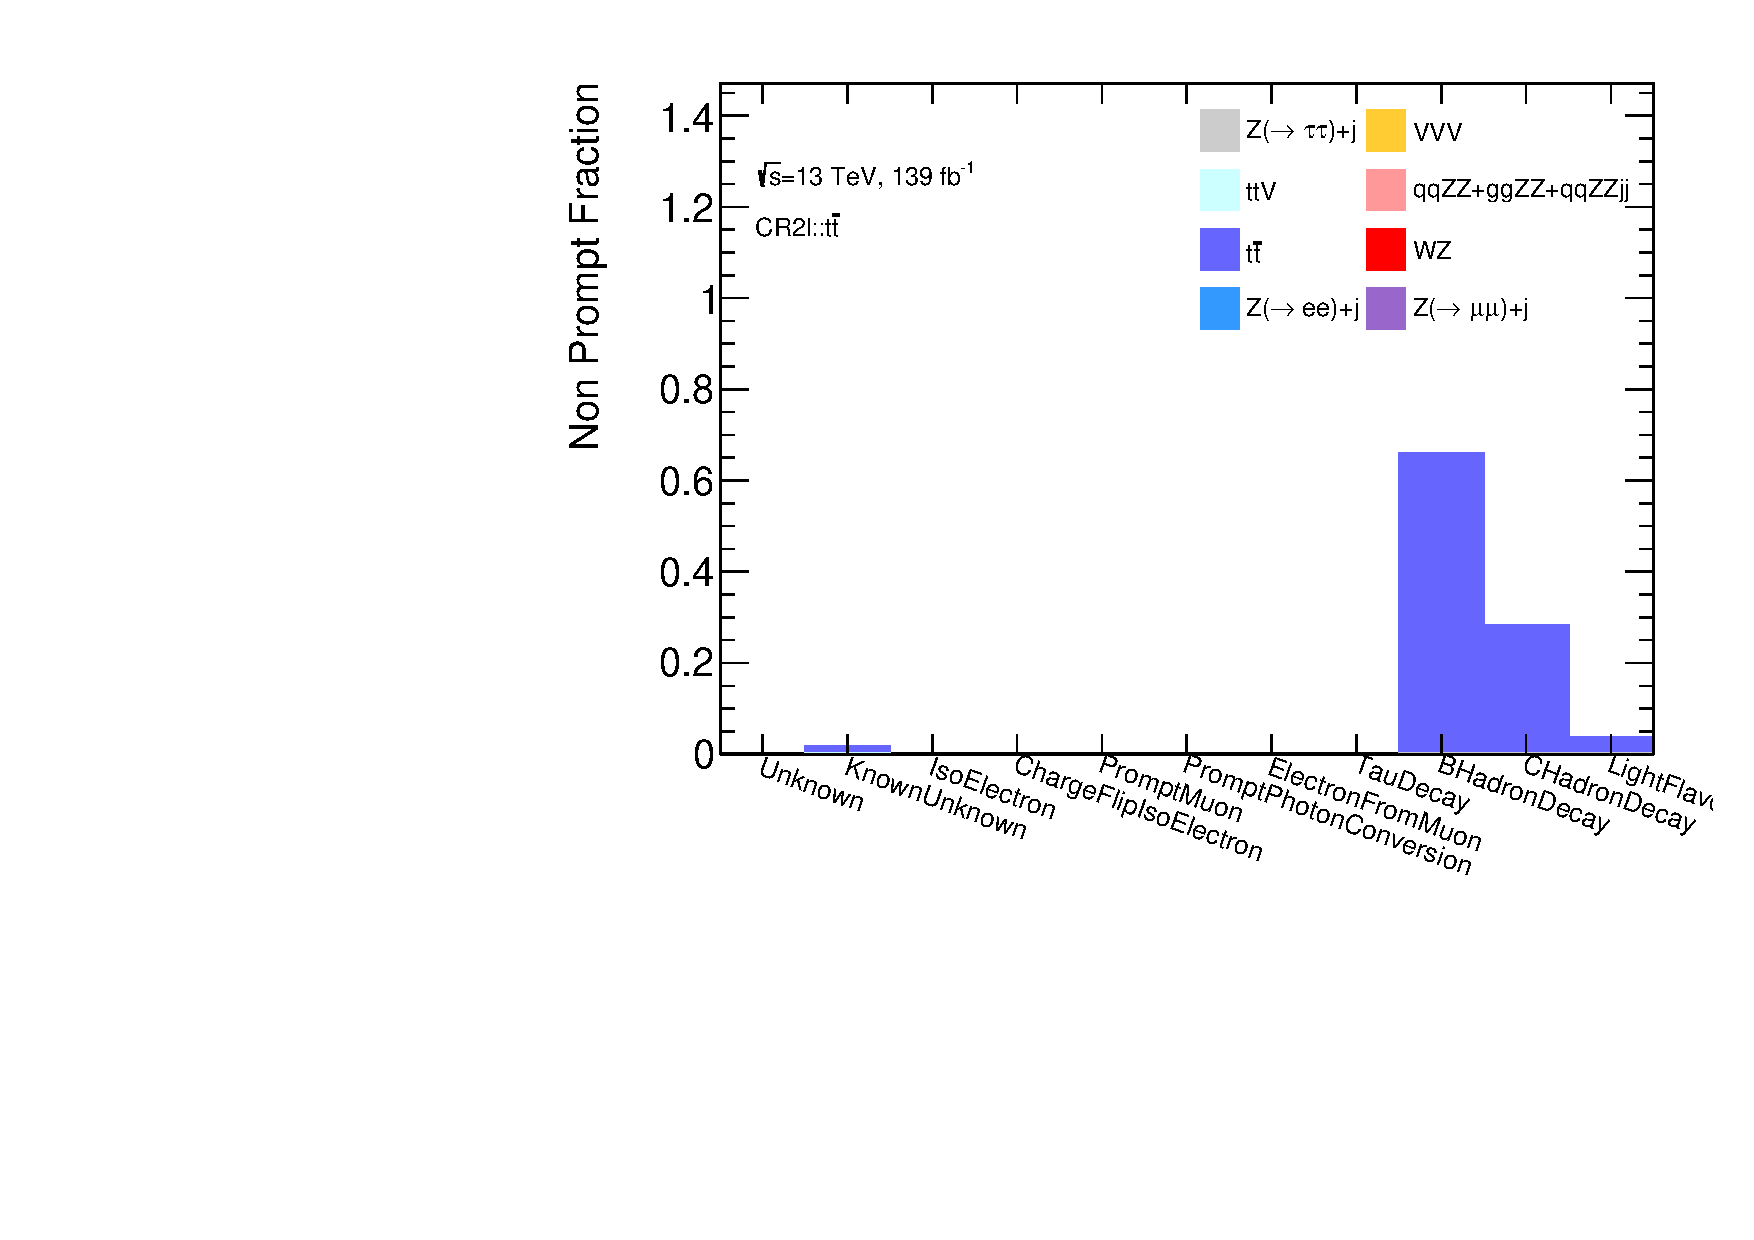
\includegraphics[width=.9\linewidth]{figures/Analysis/Background/NonPromptComposition_ttbar_Muons.pdf}
        \caption{Non-prompt muons in $t\bar{t}$ CR.}
    \end{subfigure}
        \caption{ Sources of non-prompt muons in $Z+jets$(left) and $t\bar{t}$(right) control regions.\label{fig:FakeCompositionCR2LMuon}}
\end{figure}

\begin{figure}[htb]
        \centering
        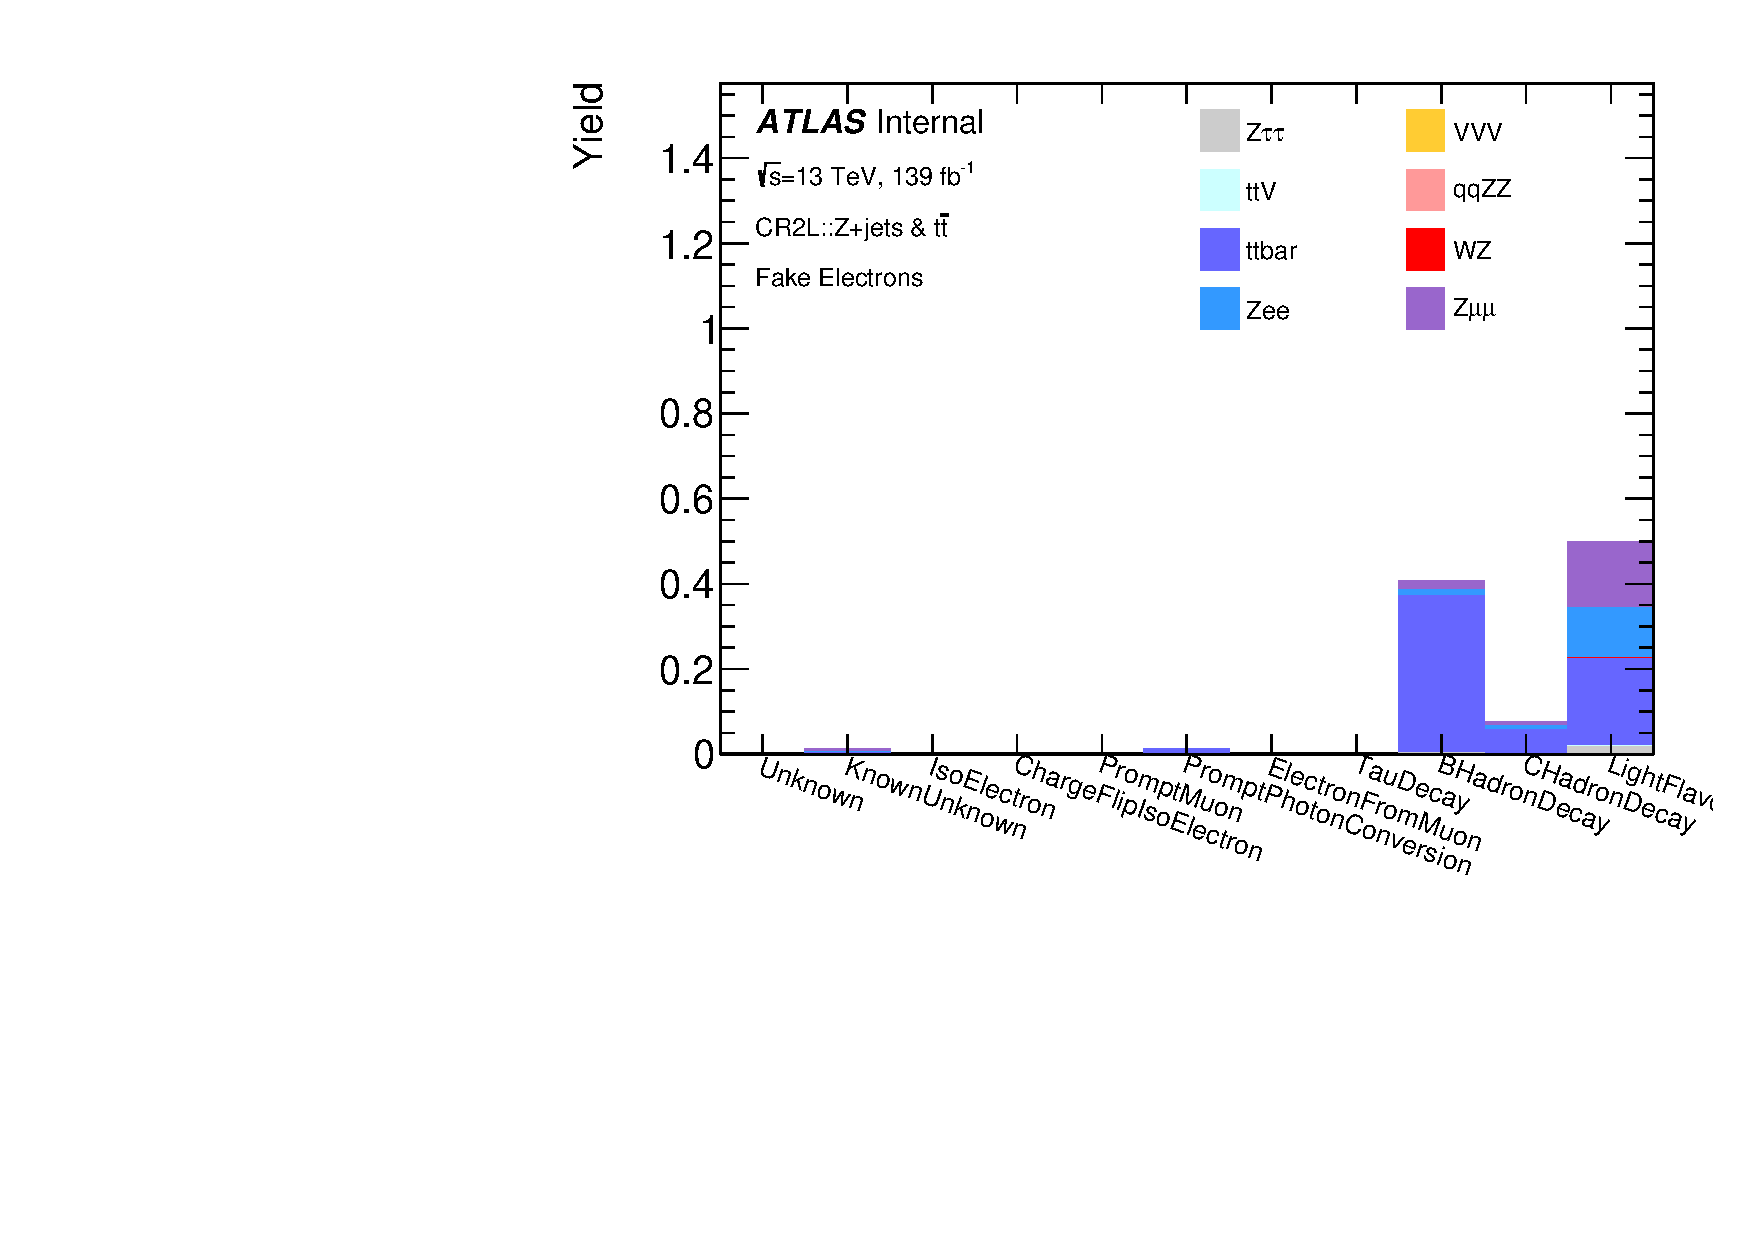
\includegraphics[width = 0.42\textwidth]{figures/Analysis/Background/NonPromptComposition_Combined_Electrons.pdf}
        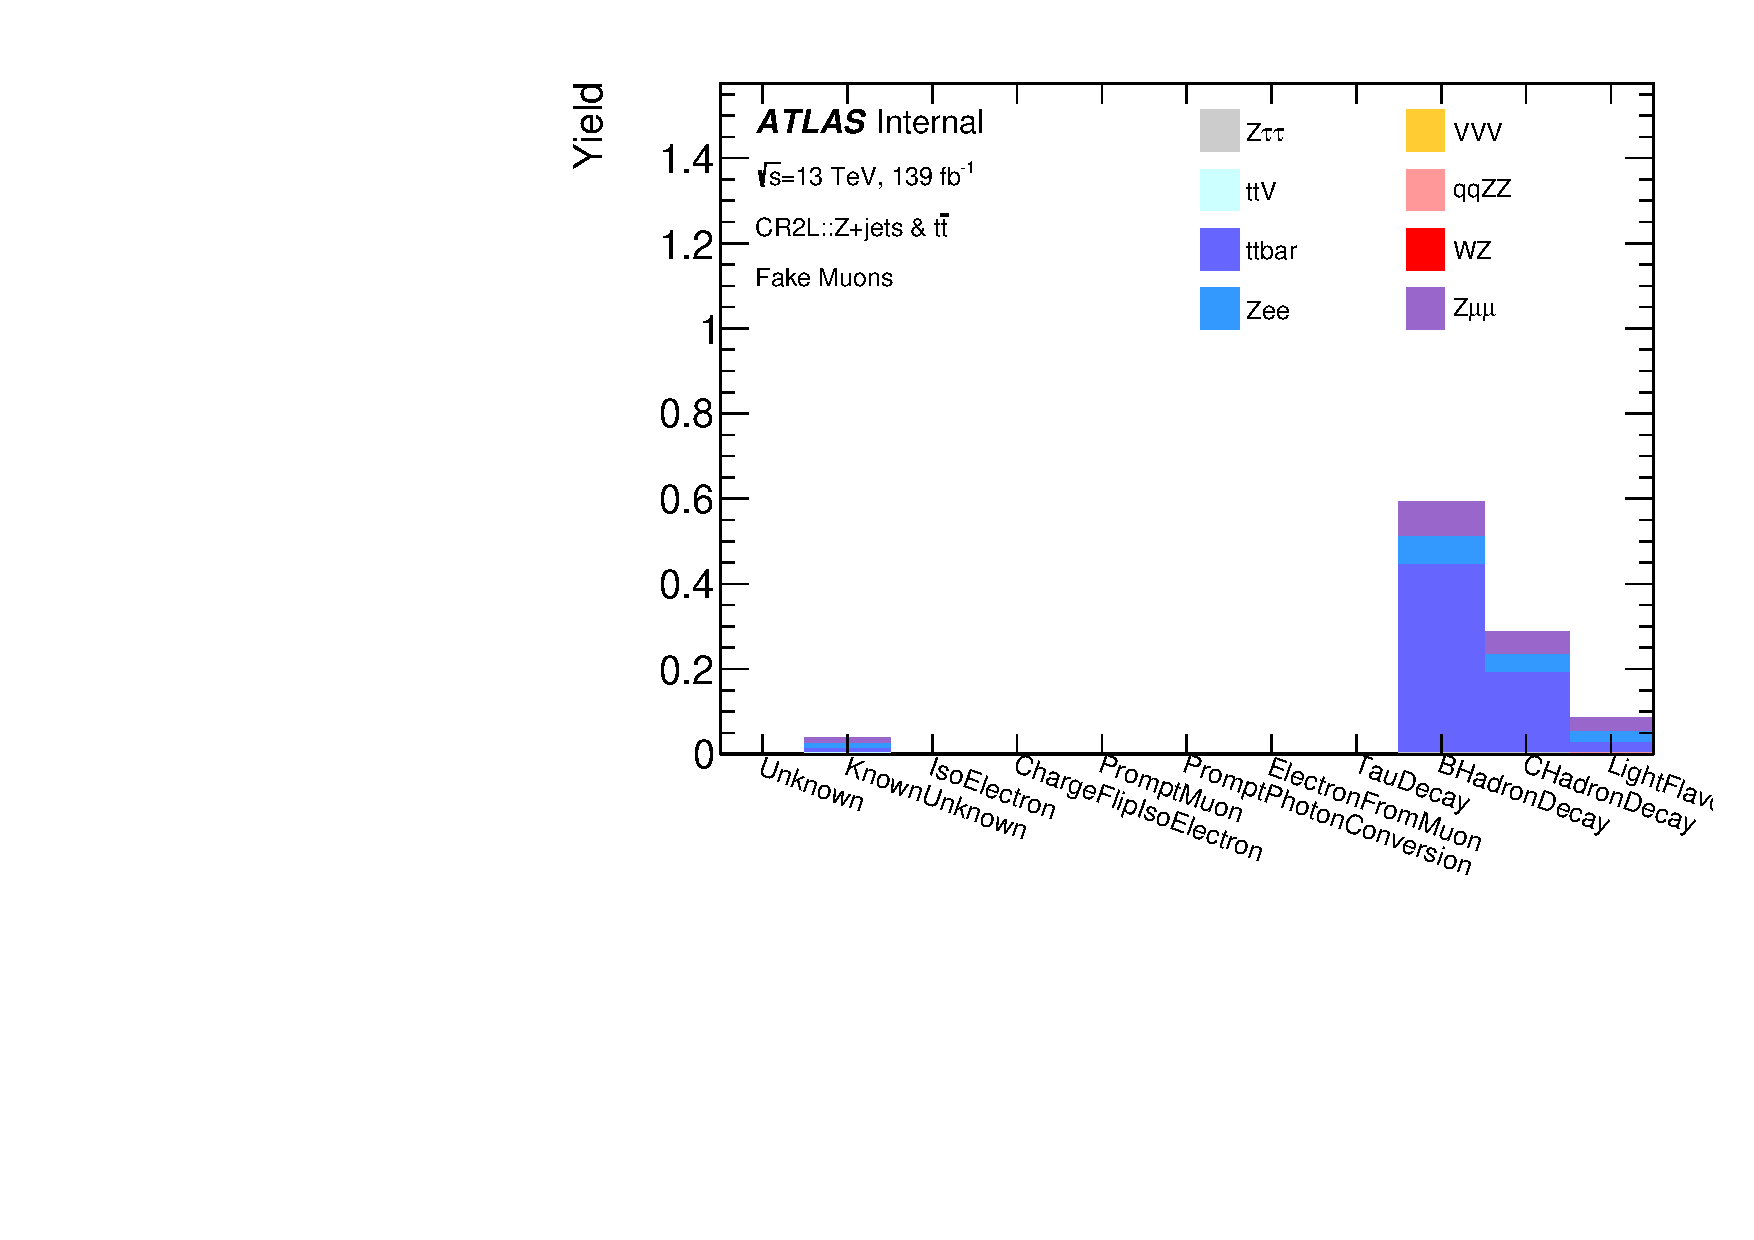
\includegraphics[width = 0.42\textwidth]{figures/Analysis/Background/NonPromptComposition_Combined_Muons.pdf}
        \caption{ Origins of non-prompt electrons (left) and muons (right) in the combined control region. \label{fig:NonPromptCombined}}
\end{figure}

The $b$-jet requirement applied to suppress the prompt-lepton contamination from the WZ process in $t\bar{t}$ CR ensures the presence of at least one jet in all events. Therefore, events without jets in the combined control region only contain the $Z+jets$ $n_{jet}~=~0$ events. The two control regions are first weighted and combined for the events with the jets to match the heavy flavor composition of the $n_{jet}~>~0$ events in the signal region. The combination weights are evaluated by solving the following equation$:$

\begin{equation}
\begin{aligned}
\frac{\{w \times N_{Z+jets} \times f_{HF, Z+jets}\} + \{ (1-w) \times N_{t\bar{t}} \times f_{HF, t\bar{t}}\}}{\{w \times N_{Z+jets} + (1-w) \times N_{t\bar{t}} \}} = f_{HF, SR}  \\
\end{aligned}
\end{equation}
where $N$ is the total yield in the control region, $ f_{HF}$ is the ratio of the non-prompt leptons from heavy-flavor decays to total non-prompt leptons, and $w$ is the combination weight to be determined.

As the composition of non-prompt electrons and muons are different in different regions, the weights are evaluated separately for electrons and muons and estimated to be $w_{\mu} = 0.26$ and $w_{e} = 0.06$. Figure \ref{fig:NonPromptCombined} shows the composition of the non-prompt electrons and muons in the combined control region, which is formed by a weighted combination of the $Z+jets$ CR and the $t\bar{t}$ CR.

Figures \ref{fig:Add_e_ZplusX} and \ref{fig:Add_e_ttbar} show the distributions of additional baseline electrons as a function of their $p_{T}$ in the $Z+jets$ CR and $t\bar{t}$ CR, respectively, whereas, \ref{fig:Add_e_combined} show the same for the combined control region. For $Z+jets$ CR at low $p_{T}$, additional baseline electrons are overestimated in MC by about $20\%$, thus, showing the precision of MC to estimate the non-prompt leptons is limited. Similarly, Figures \ref{fig:Add_mu_ZplusX}, \ref{fig:Add_mu_ttbar} and \ref{fig:Add_mu_combined} show the distributions of additional baseline muons as a function of their $p_{T}$ in the three control regions. In $Z+jets$ CR, the low $p_{T}$ additional muons mainly originate from $Z\rightarrow \ell \ell$ process, whereas the high $p_{T}$ events originate more significantly from $t\bar{t}$ and WZ processes.

\begin{figure}[htb]
    \begin{subfigure}{.48\textwidth}
        \centering
        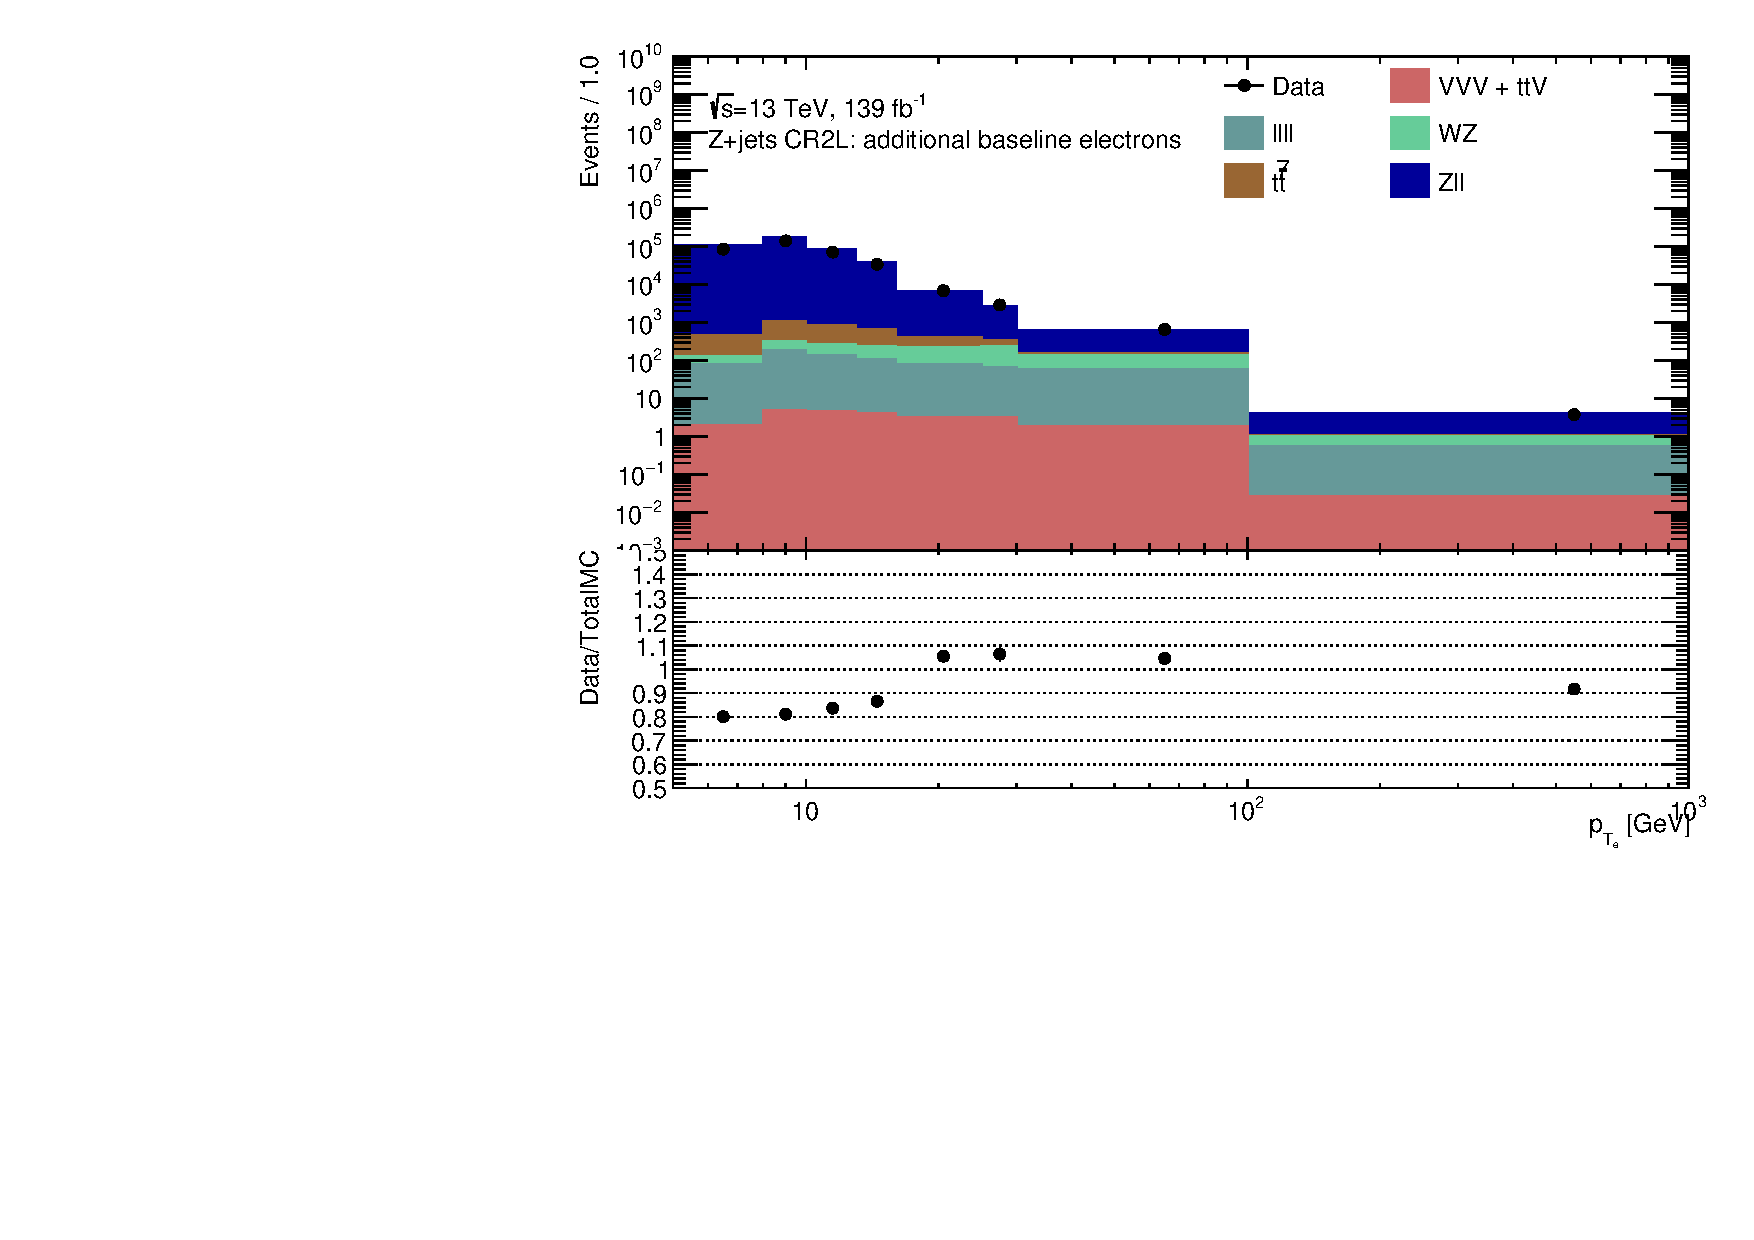
\includegraphics[width=.9\linewidth]{figures/Analysis/Background/Overlay_pt_Baseline_elecs_ZplusX.pdf}
        \caption{$Z+jets$ CR \label{fig:Add_e_ZplusX}}
    \end{subfigure}
    \begin{subfigure}{.48\textwidth}
        \centering
        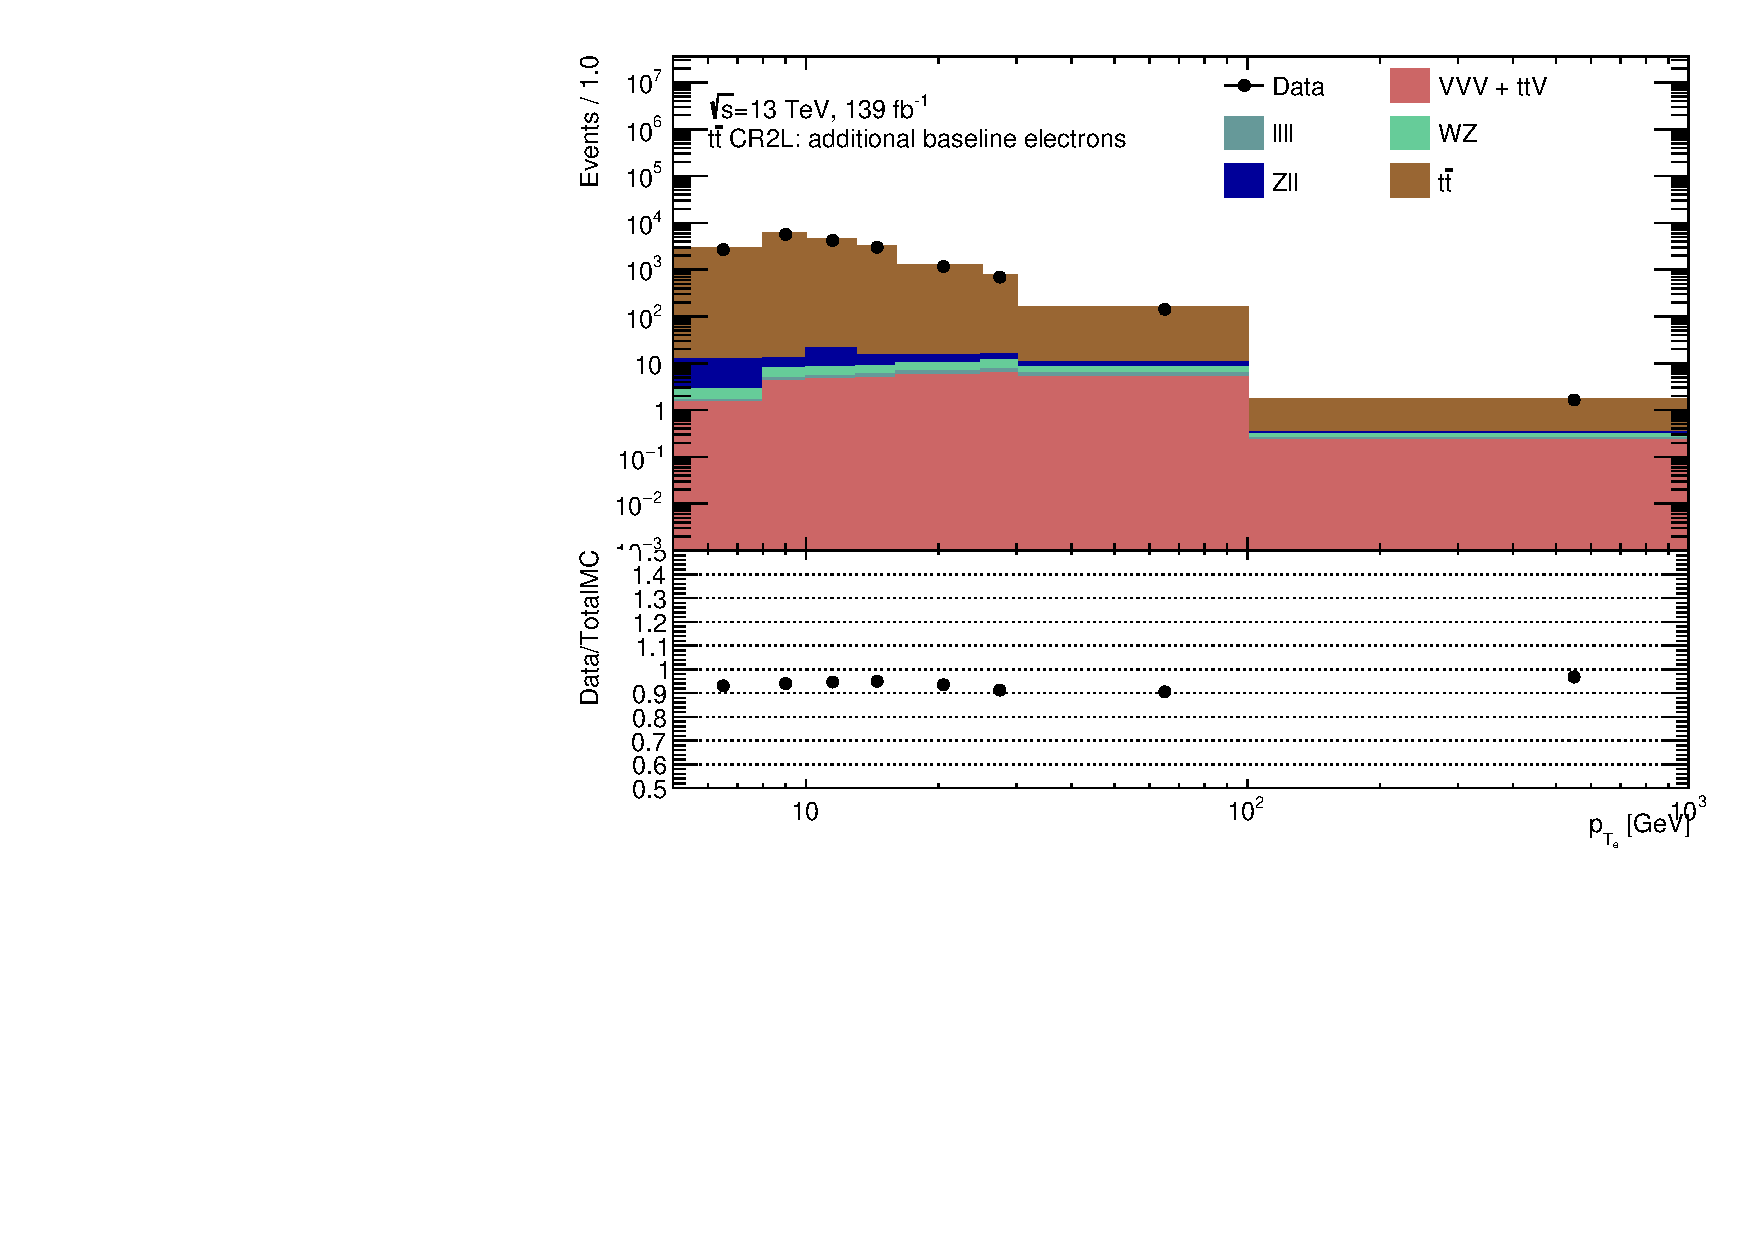
\includegraphics[width=.9\linewidth]{figures/Analysis/Background/Overlay_pt_Baseline_elecs_ttbar.pdf}
        \caption{$t\bar{t}$ CR \label{fig:Add_e_ttbar}}
    \end{subfigure}\\
    \begin{subfigure}{.48\textwidth}
        \centering
        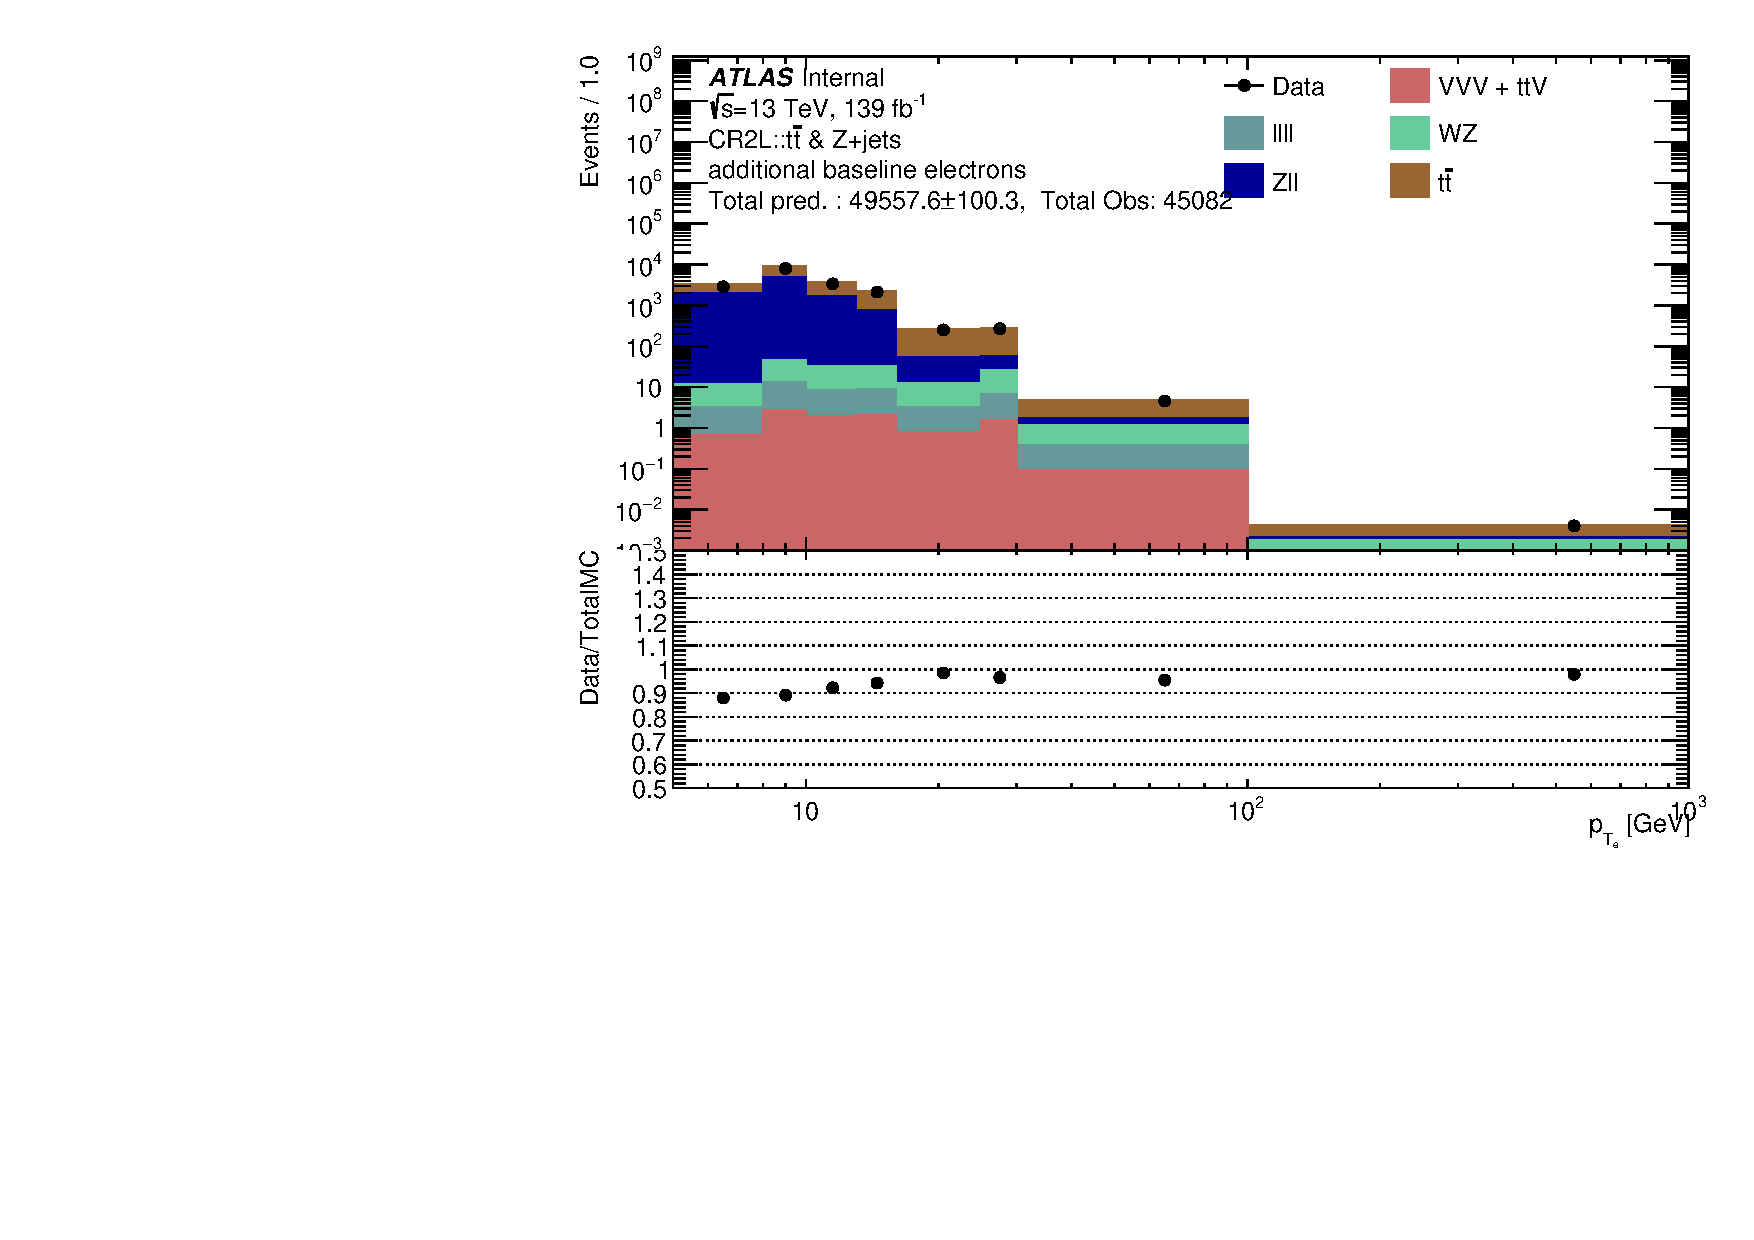
\includegraphics[width=.9\linewidth]{figures/Analysis/Background/Overlay_pt_Baseline_elecs_Combined.pdf}
        \caption{combined control region \label{fig:Add_e_combined}}
    \end{subfigure}
        \caption{ Additional baseline electrons as a function of $p_{T}$ in control regions. \label{fig:ControlRegionsAdditionalBaselineElectronpT}}
\end{figure}

\begin{figure}[htb]
    \begin{subfigure}{.48\textwidth}
        \centering
        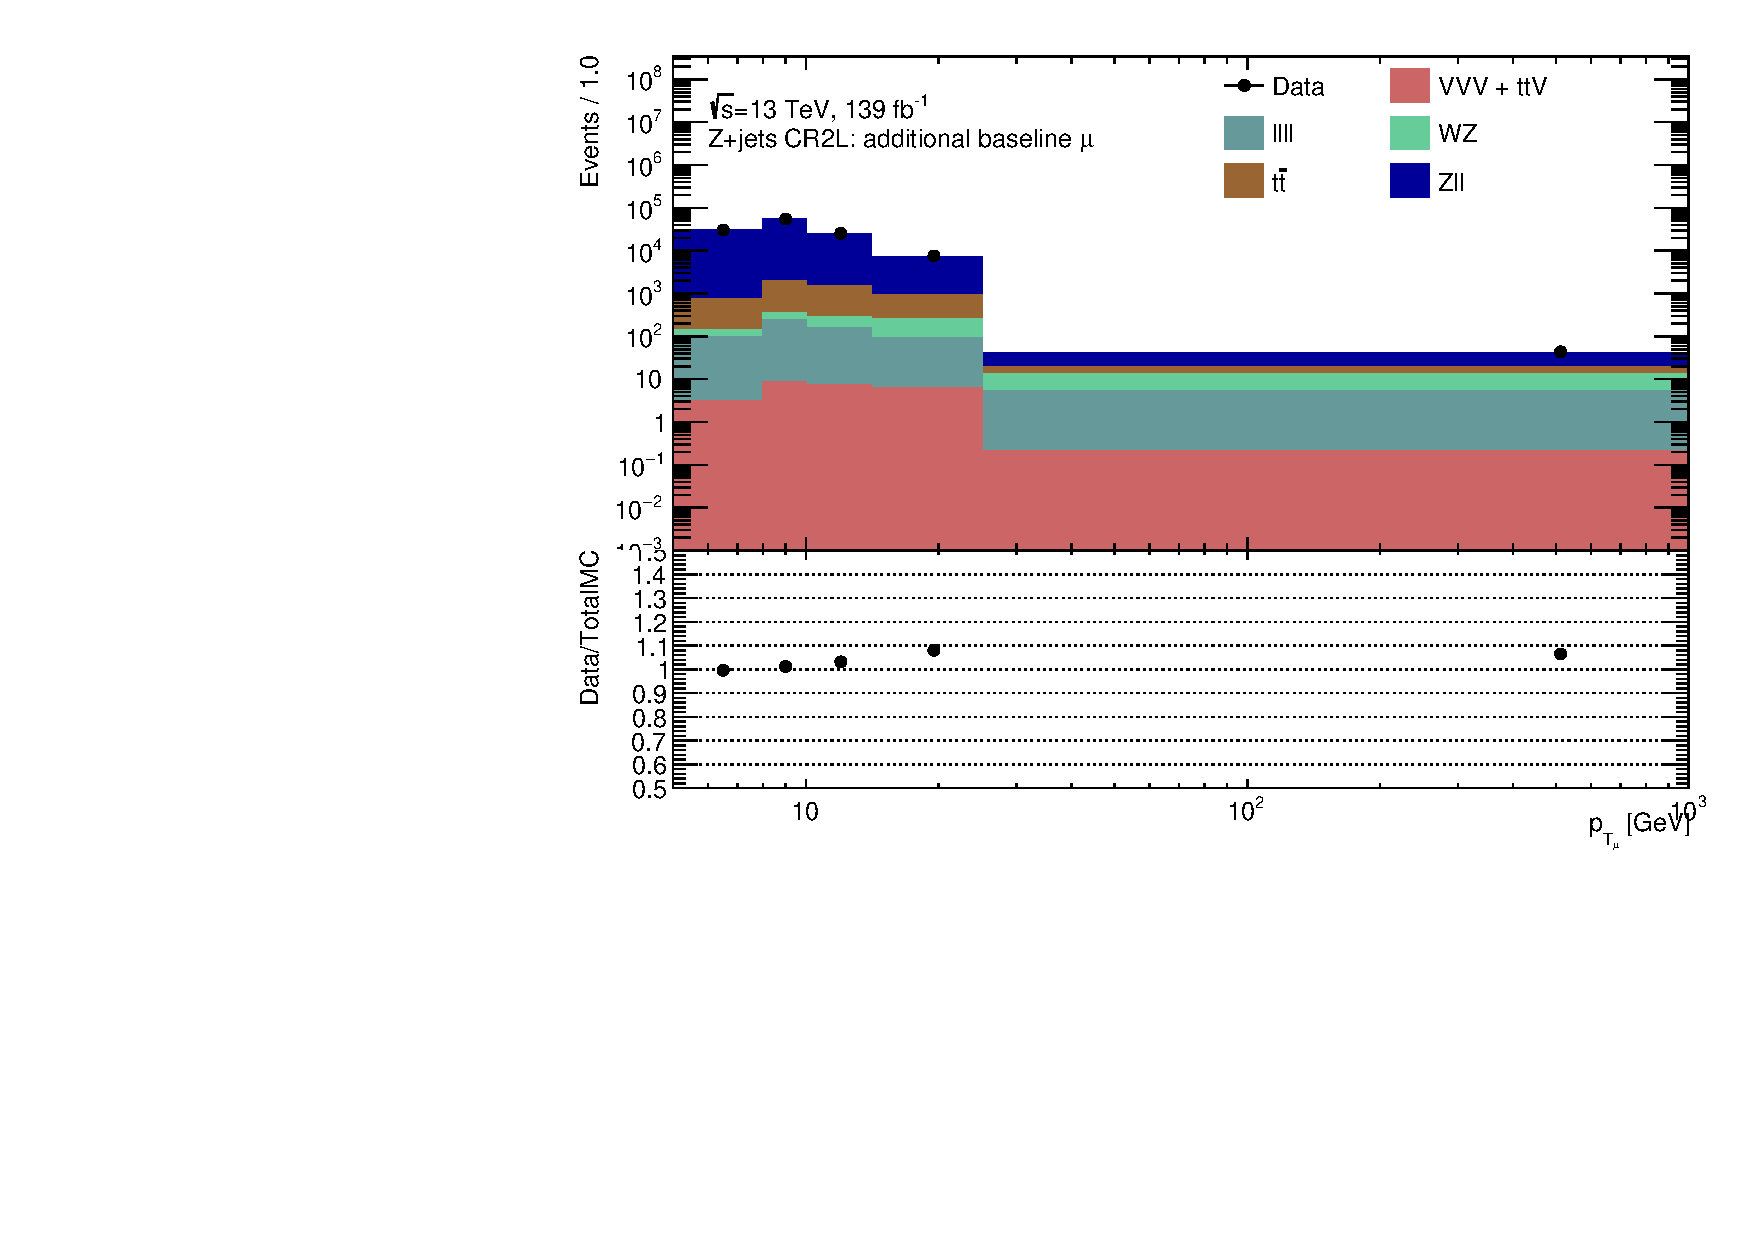
\includegraphics[width=.9\linewidth]{figures/Analysis/Background/Overlay_pt_Baseline_muons_ZplusX.pdf}
        \caption{$Z+jets$ CR \label{fig:Add_mu_ZplusX}}
    \end{subfigure}
    \begin{subfigure}{.48\textwidth}
        \centering
        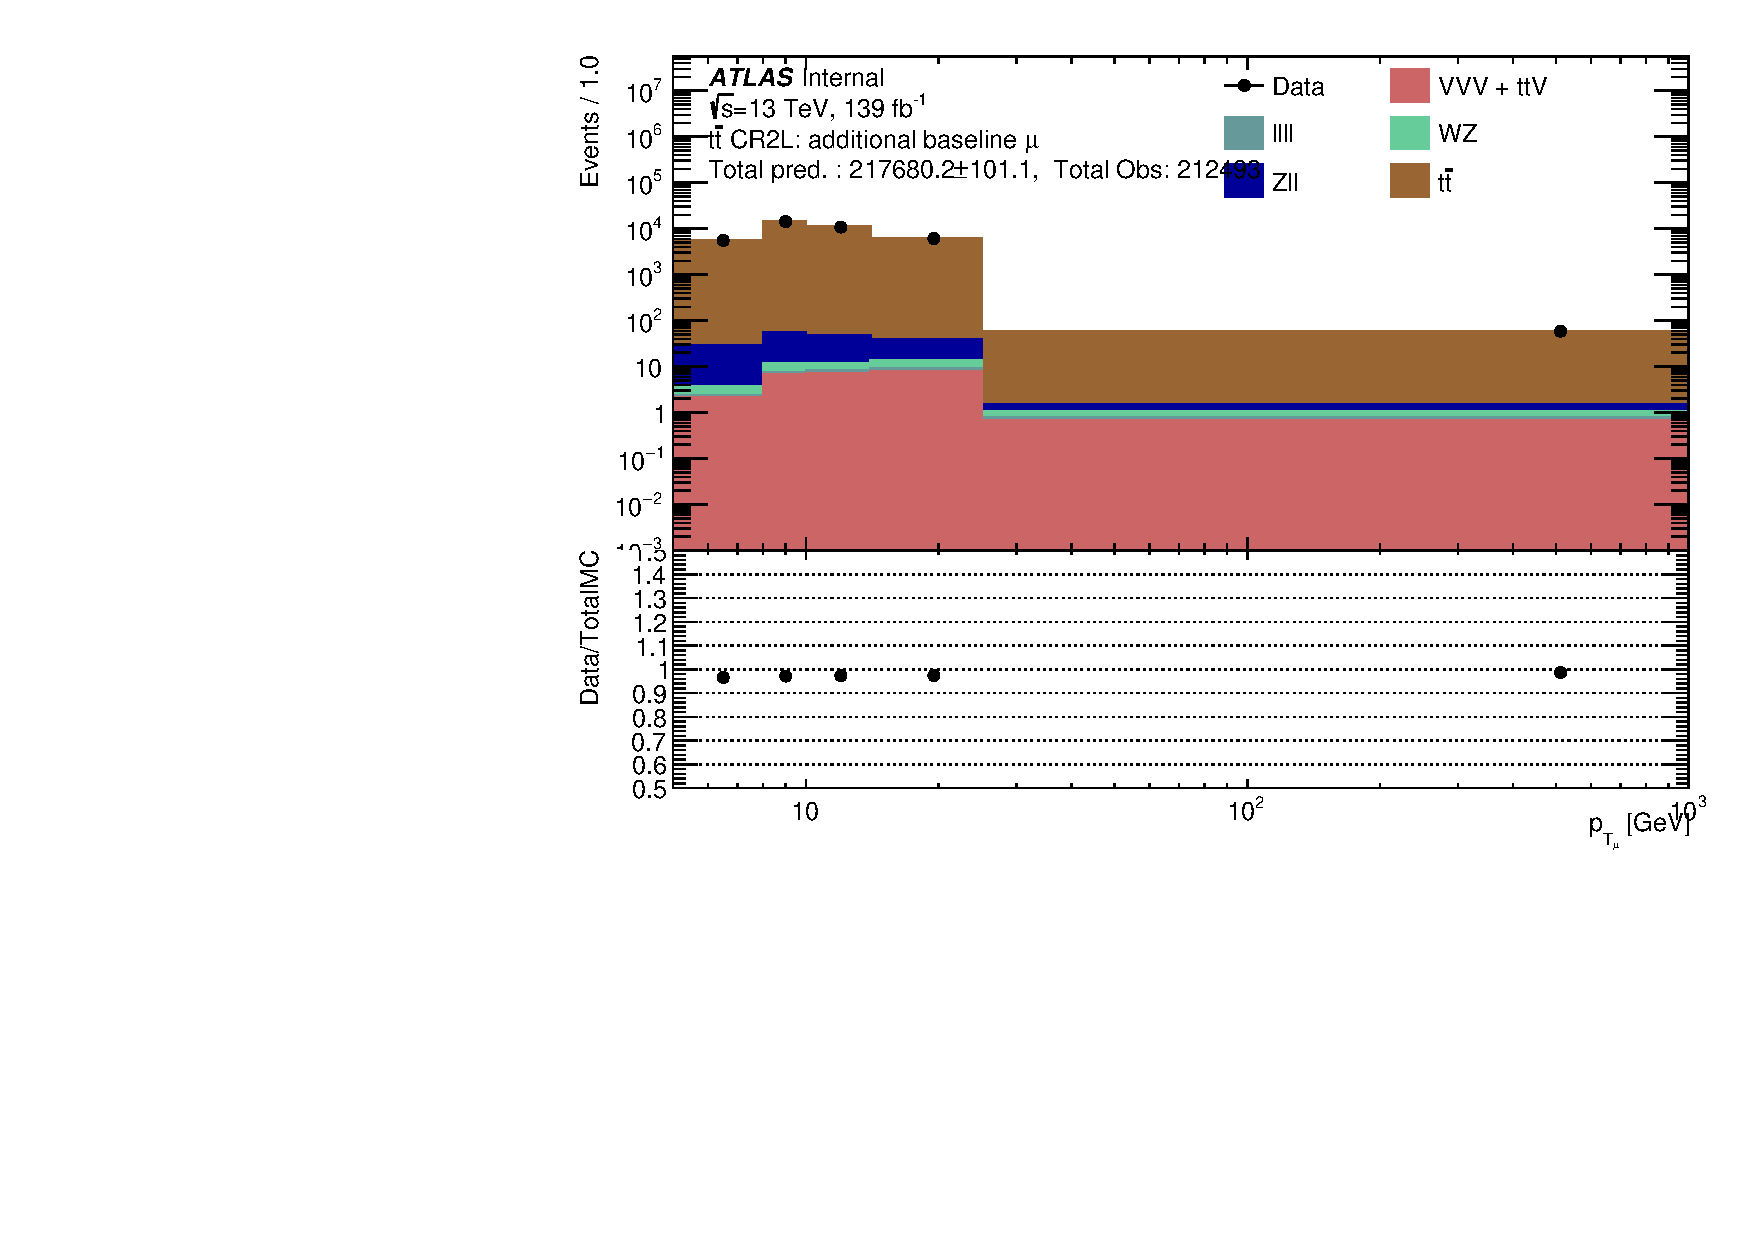
\includegraphics[width=.9\linewidth]{figures/Analysis/Background/Overlay_pt_Baseline_muons_ttbar.pdf}
        \caption{$t\bar{t}$ CR \label{fig:Add_mu_ttbar}}
    \end{subfigure} \\
    \begin{subfigure}{.48\textwidth}
        \centering
        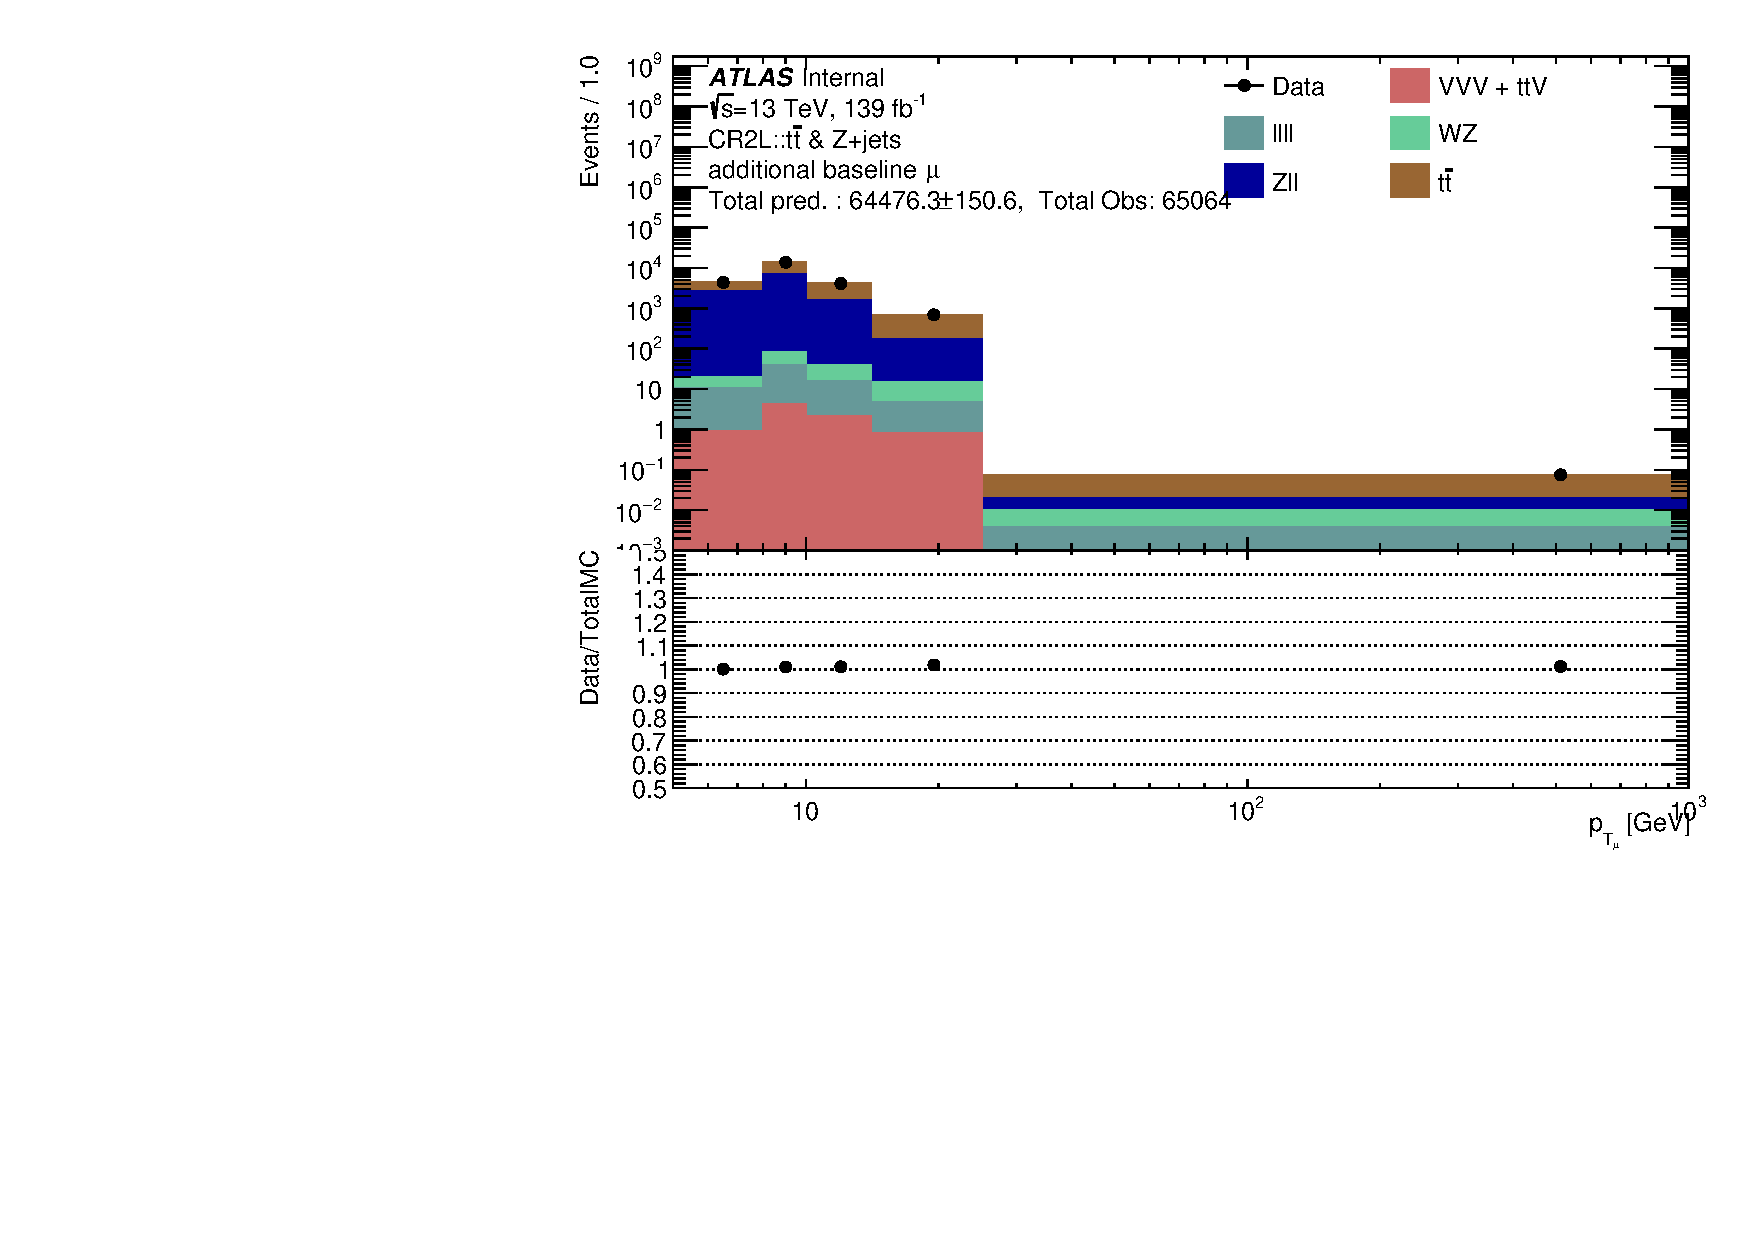
\includegraphics[width=.9\linewidth]{figures/Analysis/Background/Overlay_pt_Baseline_muons_Combined.pdf}
        \caption{combined control region \label{fig:Add_mu_combined}}
    \end{subfigure}
        \caption{ Additional baseline muons as a function of $p_{T}$ in control regions. \label{fig:ControlRegionsAdditionalBaselineMuonpT}}
\end{figure}

\subsubsection{ Fake Factor Strategy }
\label{subsubsec:EstimationStrategy}

The centrally developed \textit{fake factor tool} by ATLAS IFF is used to estimate the fake background \cite{FakeBkgTool}. The tool takes the ratio of signal to baseline leptons, i.e., \textit{fake efficiency (f)}, calculated in the combined control region as an input where,

\begin{equation}
f = \frac{N_{non-prompt~signal~leptons}}{N_{non-prompt~baseline~leptons}}
\end{equation}

For a simple case of a signal region with one signal lepton, the observed signal lepton ($N^{T}$) and baseline-anti-signal lepton ($N^{L}$) can be estimated in terms of the number of prompt or real baseline leptons ($N^{B}_{R}$) and the number of non-prompt or fake baseline leptons ($N^{B}_{F}$) as

\begin{equation}
N^{T} = rN^{B}_{R}+fN^{B}_{F}
\label{eqn:NoOfTight}
\end{equation}
and 
\begin{equation}
N^{L} = (1-r)N^{B}_{R} + (1-f)N^{B}_{F}
\label{eqn:NoOfLoose}
\end{equation}
where, $r$ is the \textit{real efficiency} such that, 
\begin{equation} 
    r=\frac{N_{prompt~signal~leptons}}{N_{prompt~baseline~leptons}}
\end{equation}

Equations \ref{eqn:NoOfTight} and \ref{eqn:NoOfLoose} can be written as a $2 \times 2$ matrix equation as

\begin{equation}
    \begin{pmatrix} N^{T} \\ N^{L} \end{pmatrix} =  \begin{pmatrix} r & f \\ 1-r & 1-f \end{pmatrix} \begin{pmatrix} N^{B}_{R} \\ N^{B}_{F}\end{pmatrix}
    \label{eqn:RealFakeLepton}
\end{equation}

The number of non-prompt baseline contributions is estimated by ignoring the higher-order term of the fake efficiency as

\begin{equation}
    N_{F}^{B} =  \frac{1}{r-f}[r(N^{T}+N^{L})-N^{T}]
    \label{eqn:NfakeBaseline}
\end{equation}
Therefore, the predicted number of non-prompt signal lepton is 

\begin{equation}
    N_{F}^{T} =  \frac{f}{r-f}[r(N^{T}+N^{L})-N^{T}]
\label{eqn:NfakeSignal}
\end{equation}

The fake factor method assumes the $r\rightarrow 1$ limit, which simplifies equation \ref{eqn:NfakeSignal}. However, since the real efficiency of any measurement is less than one, this approximation overestimates the fake background. To account for this overestimation, the number of genuine baseline-anti-signal prompt leptons ($N^{L}_{R}$) are measured in MC and subtracted to get the final background yield as, 

\begin{equation}
    N_{F}^{T} =  \frac{f}{1-f}[N^{L}-N^{L}_{R}]
\label{eqn:NfakeSignalFinal}
\end{equation}
where, the coefficient \begin{equation} F=\frac{f}{1-f} \label{eqn:FakeFactor}
\end{equation} is the fake factor $F$. The method makes a typically safe assumption that the real anti-signal prompt leptons are modeled precisely in MC. As the fake efficiency $f$ is estimated from data in the combined control region, the fake factor background estimation method does not rely on any efficiencies or yield in the tight signal region.

This method can be extended to the four-lepton signal region where there are four baseline leptons, of which one or more could be non-prompt. Corresponding to the permutation of individual leptons to be either signal or baseline-anti-signal, there are $2^{4}=16$ \{$N^{TTTT}$, $N^{TTTL}$, $N^{TTLL}$,...$N^{LLLL}$ \} observations to consider. The analysis considers $N^{TTTT}$ the signal region; therefore, the background is estimated from the quadruplets with at least one baseline-anti-signal lepton.

\subsubsection{Fake Efficiency $\&$ Systematics}
\label{subsubsec:FakeEff}
Fake efficiency (f), defined in previous Section \ref{subsubsec:EstimationStrategy}, is evaluated from the combined control region using the total number of additional leptons from data as
\begin{equation}{\label{eq:fakeff}}
\begin{aligned}
f = \frac{ N_{Data}^{Signal}~-~N_{MC}^{Prompt~Signal}}{ N_{Data}^{Baseline}~-~N_{MC}^{Prompt~Baseline}}
\end{aligned}
\end{equation}
Since some additional leptons could originate from prompt sources, such contributions are estimated from MC and subtracted as shown in equation \ref{eq:fakeff}.

Figures \ref{fig:FakeFractionBaseline}, \ref{fig:ControlRegionsAdditionalBaselineElectronpT}, and \ref{fig:ControlRegionsAdditionalBaselineMuonpT} show that the fake-fraction and the total yield of the additional leptons are dependent on their transverse momentum $p_{T}$. Therefore, the fake efficiency evaluated using equation \ref{eq:fakeff} depends on the lepton $p_{T}$. Because of the low resolution of the detector in forward regions, a higher number of non-prompt leptons are expected in this region; thus, the fake efficiency depends on the leptons' pseudorapidity ($\eta$). Additionally, since the non-prompt leptons predominantly originate from jets, the fake efficiency also depends on the number of jets ($n_{jets}$) in an event. 

Figures \ref{fig:FakeEff_1D_Electron} and \ref{fig:FakeEff_1D_Muon} show the fake efficiencies for electrons and muons respectively as a function of $p_{T}$ (top-left), $\eta$ (top-right) and $n_{jets}$ (bottom-center). In the case of the electrons, the fake efficiency first decreases with its $p_{T}$ up to $20$ GeV and increases. Since the high-$p_{T}$ muons are most likely to originate from a prompt source, fake efficiency typically decreases as a function of $p_{T}$ for the muons. The dependency on $\eta$ is most likely from lower detector resolution causing a higher number of misidentifications and lower efficiency for TTVA.

As discussed in Section \ref{subsec:OR}, the lepton-favored overlap removal used in the analysis rejects jets if they overlap with leptons. Due to the $b-jet$ requirement in $t\bar{t}$ CR, the $njet=0$ events only consist of contributions from the $Z+jets$ CR, which does not have an explicit event requirement on the number of jets. The probability of non-prompt leptons passing the isolation requirement is higher in events with no jets or surrounding hadronic activity. Therefore, as observed, a higher fake efficiency is expected in events without jets.  

\begin{figure}[htb]
        \begin{center}
        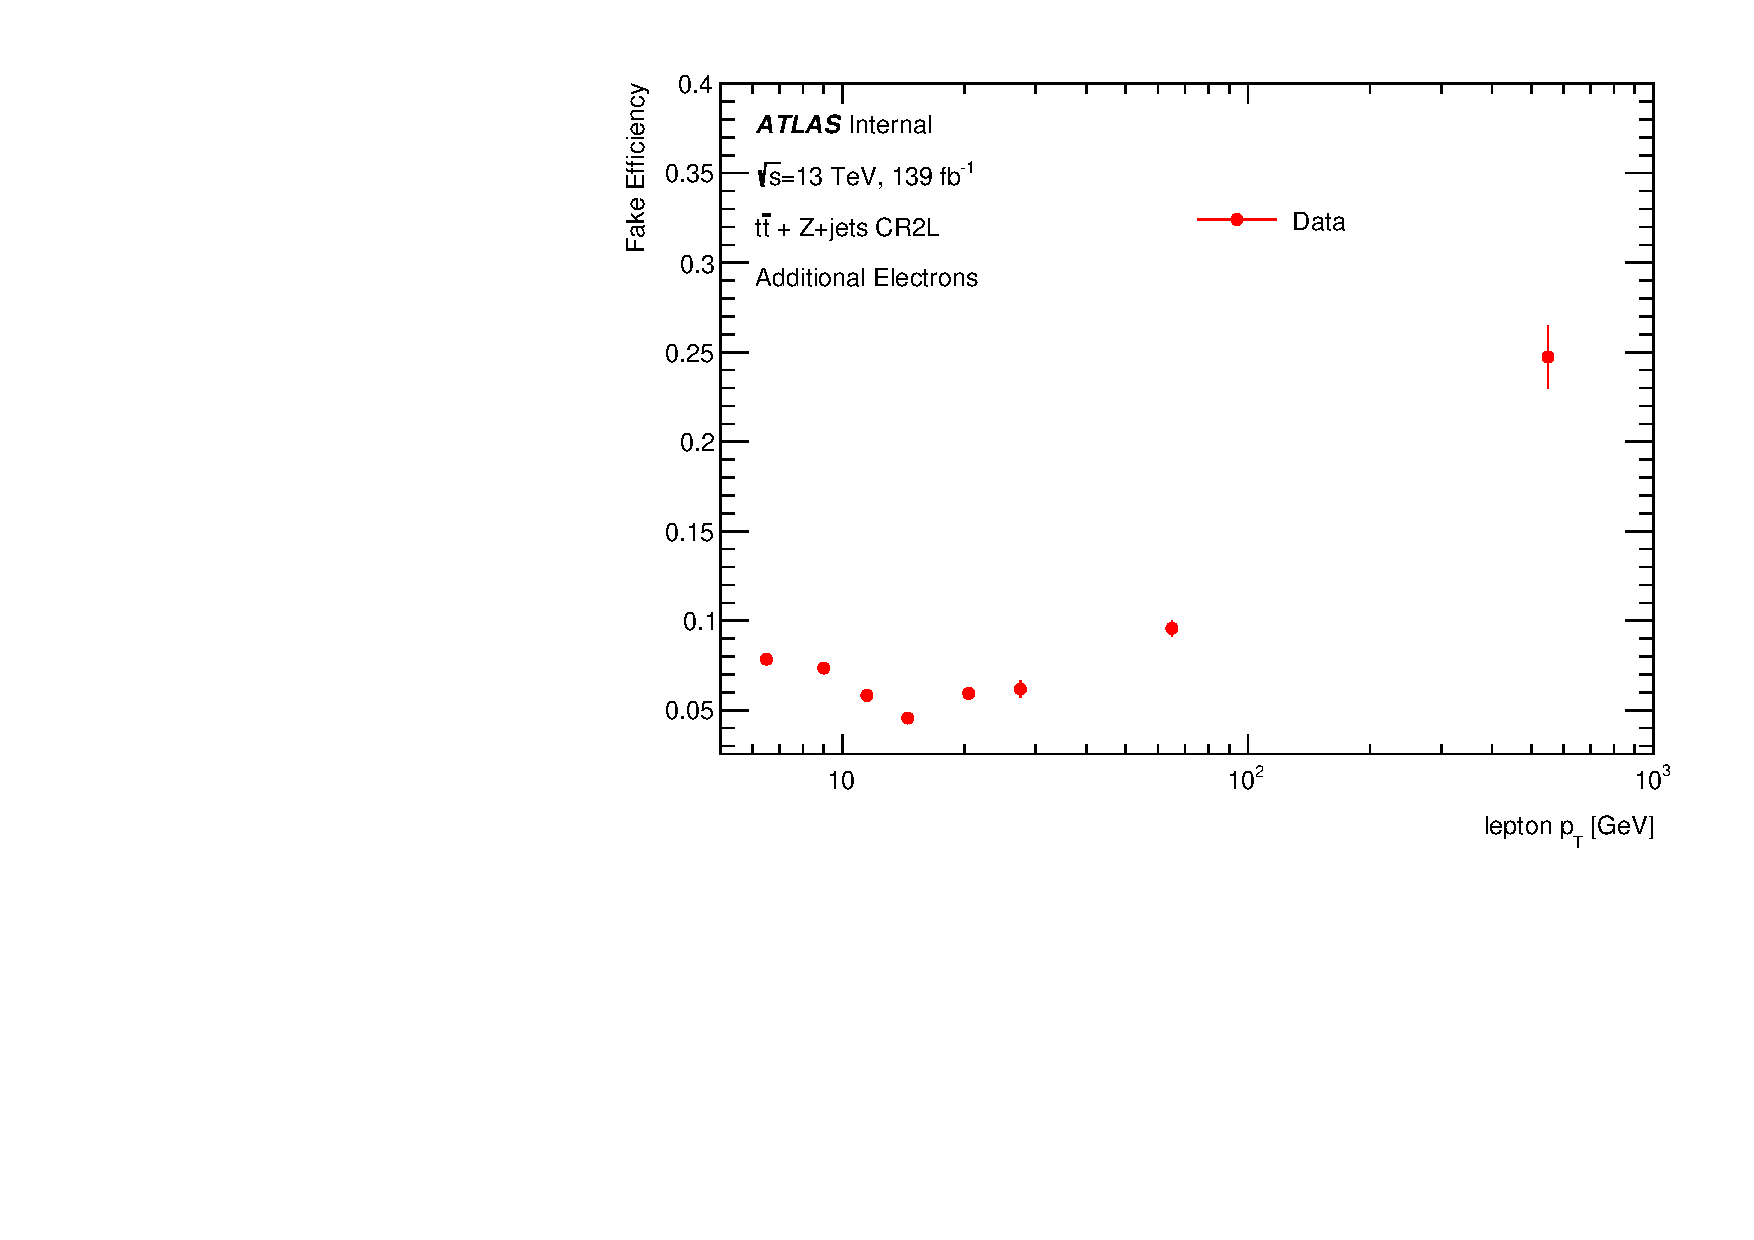
\includegraphics[width = 0.49\textwidth]{figures/Analysis/Background/Fake_Eff_Elec_pt_1D.pdf}
        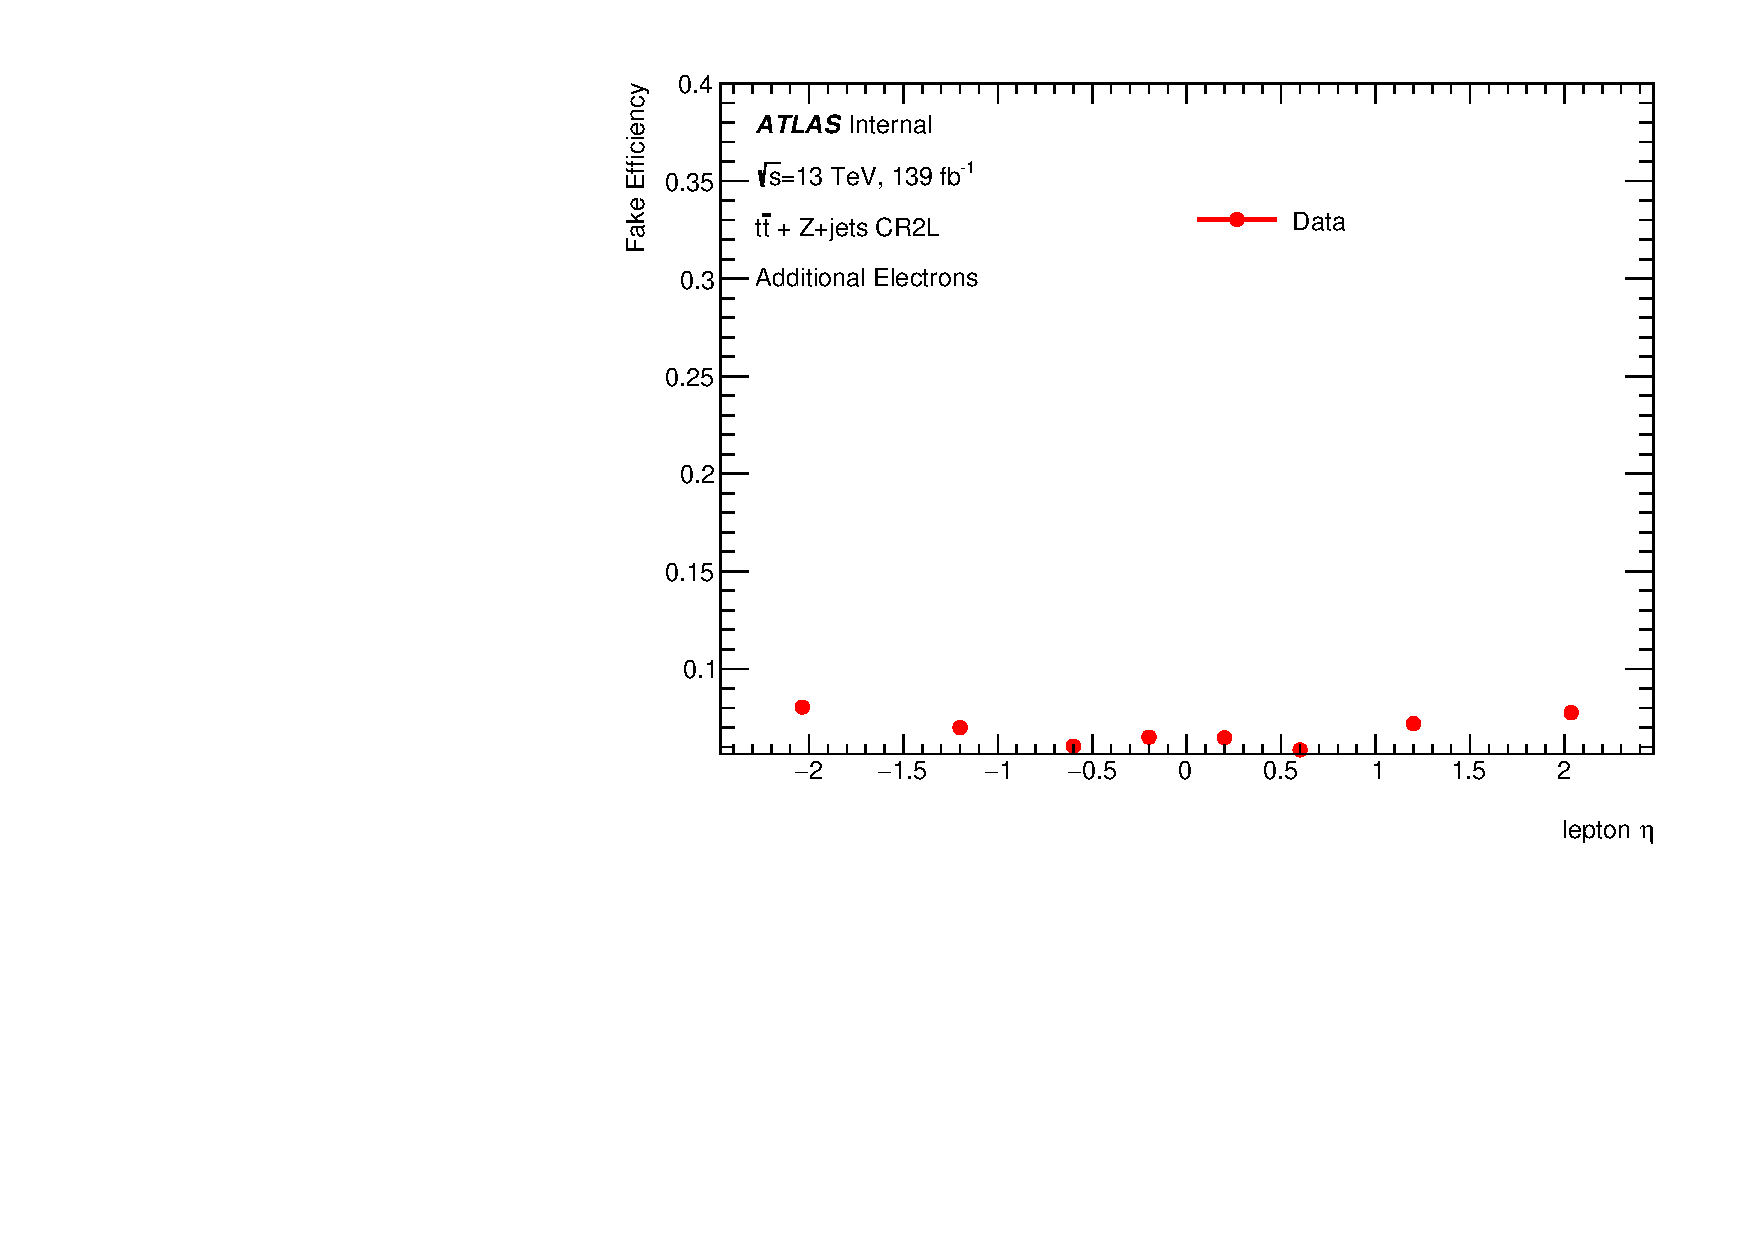
\includegraphics[width = 0.49\textwidth]{figures/Analysis/Background/Fake_Eff_Elec_eta_1D.pdf}\\
        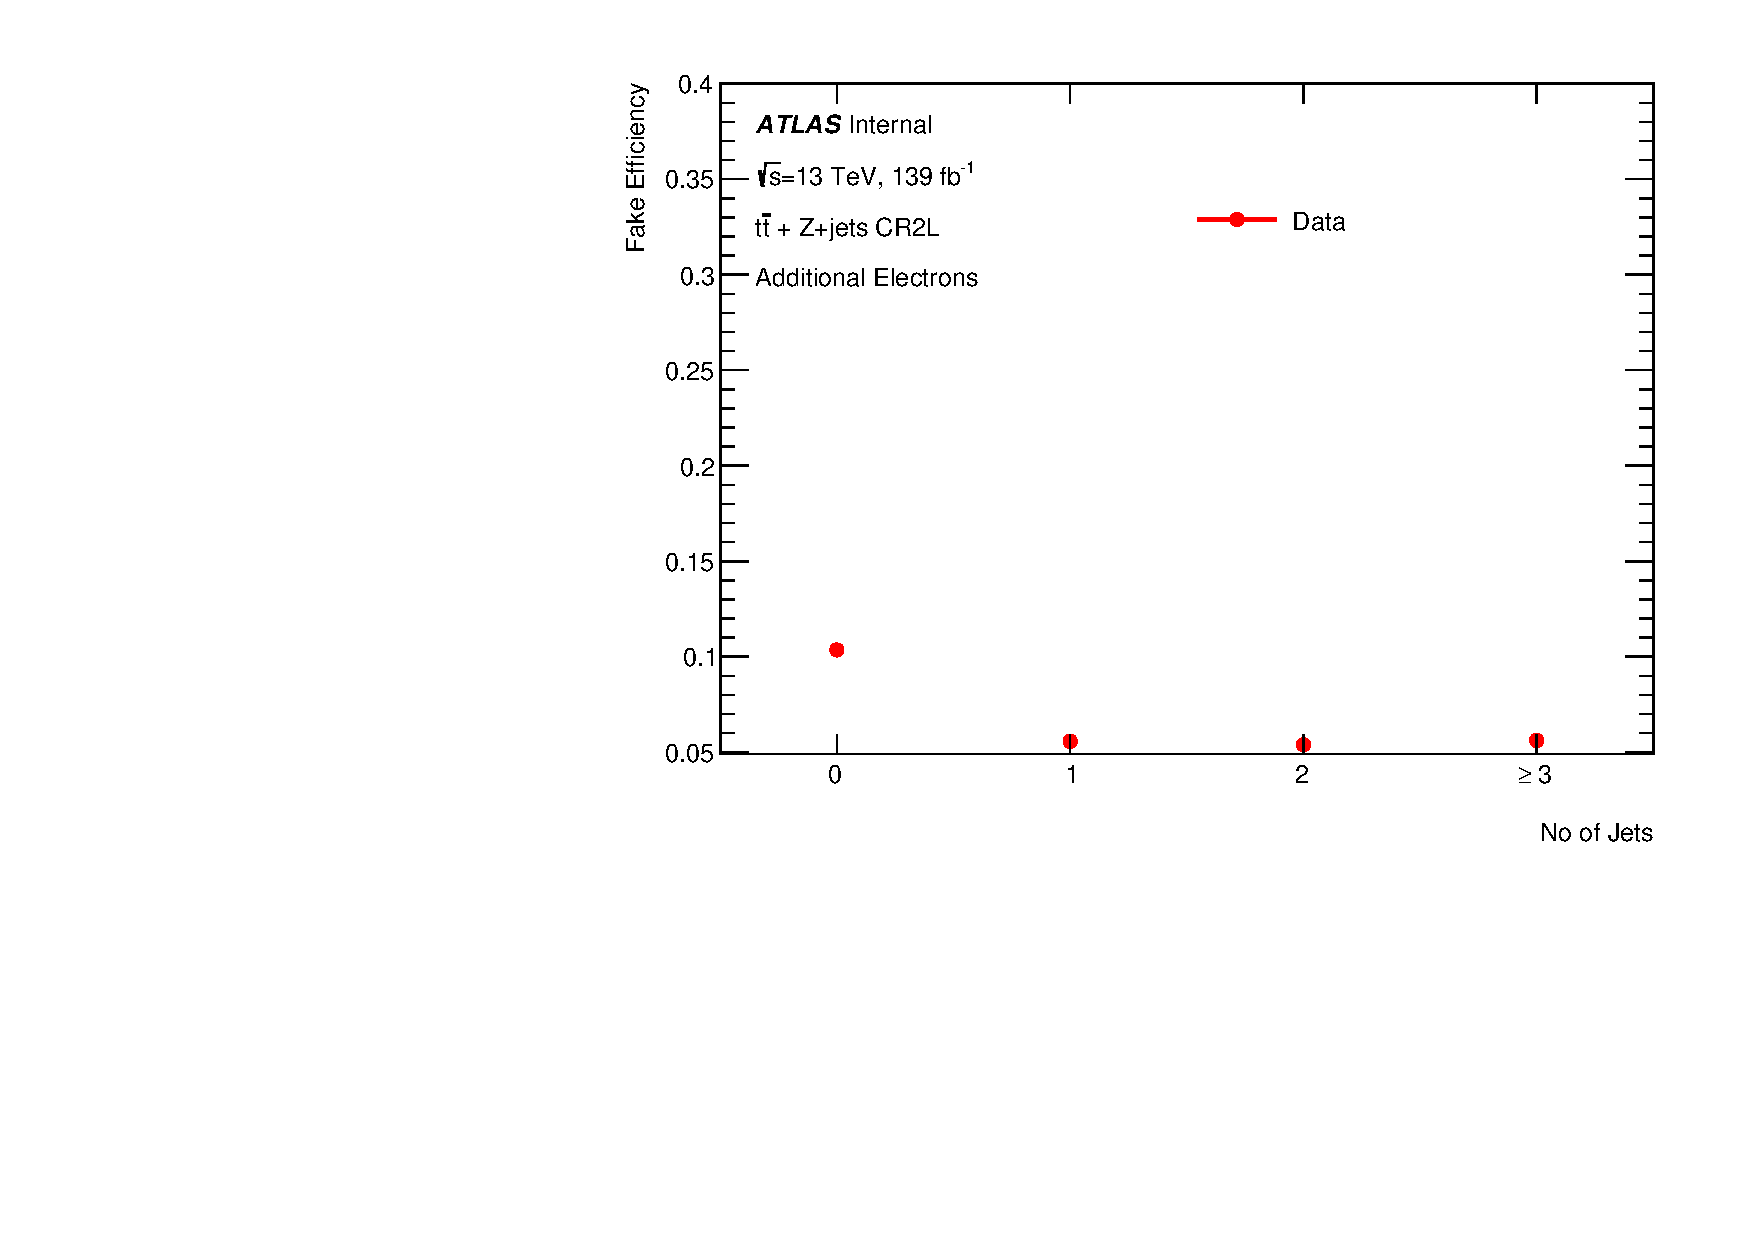
\includegraphics[width = 0.49\textwidth]{figures/Analysis/Background/Fake_Eff_Elec_jet_n_1D.pdf} 
        \end{center}
    \caption{Fake efficiency of fake electrons measured in the combined control region from data as a function of its $p_{T}$, $\eta$, and $n_{jets}$.\label{fig:FakeEff_1D_Electron}}
\end{figure}

\begin{figure}[htb]
        \begin{center}
        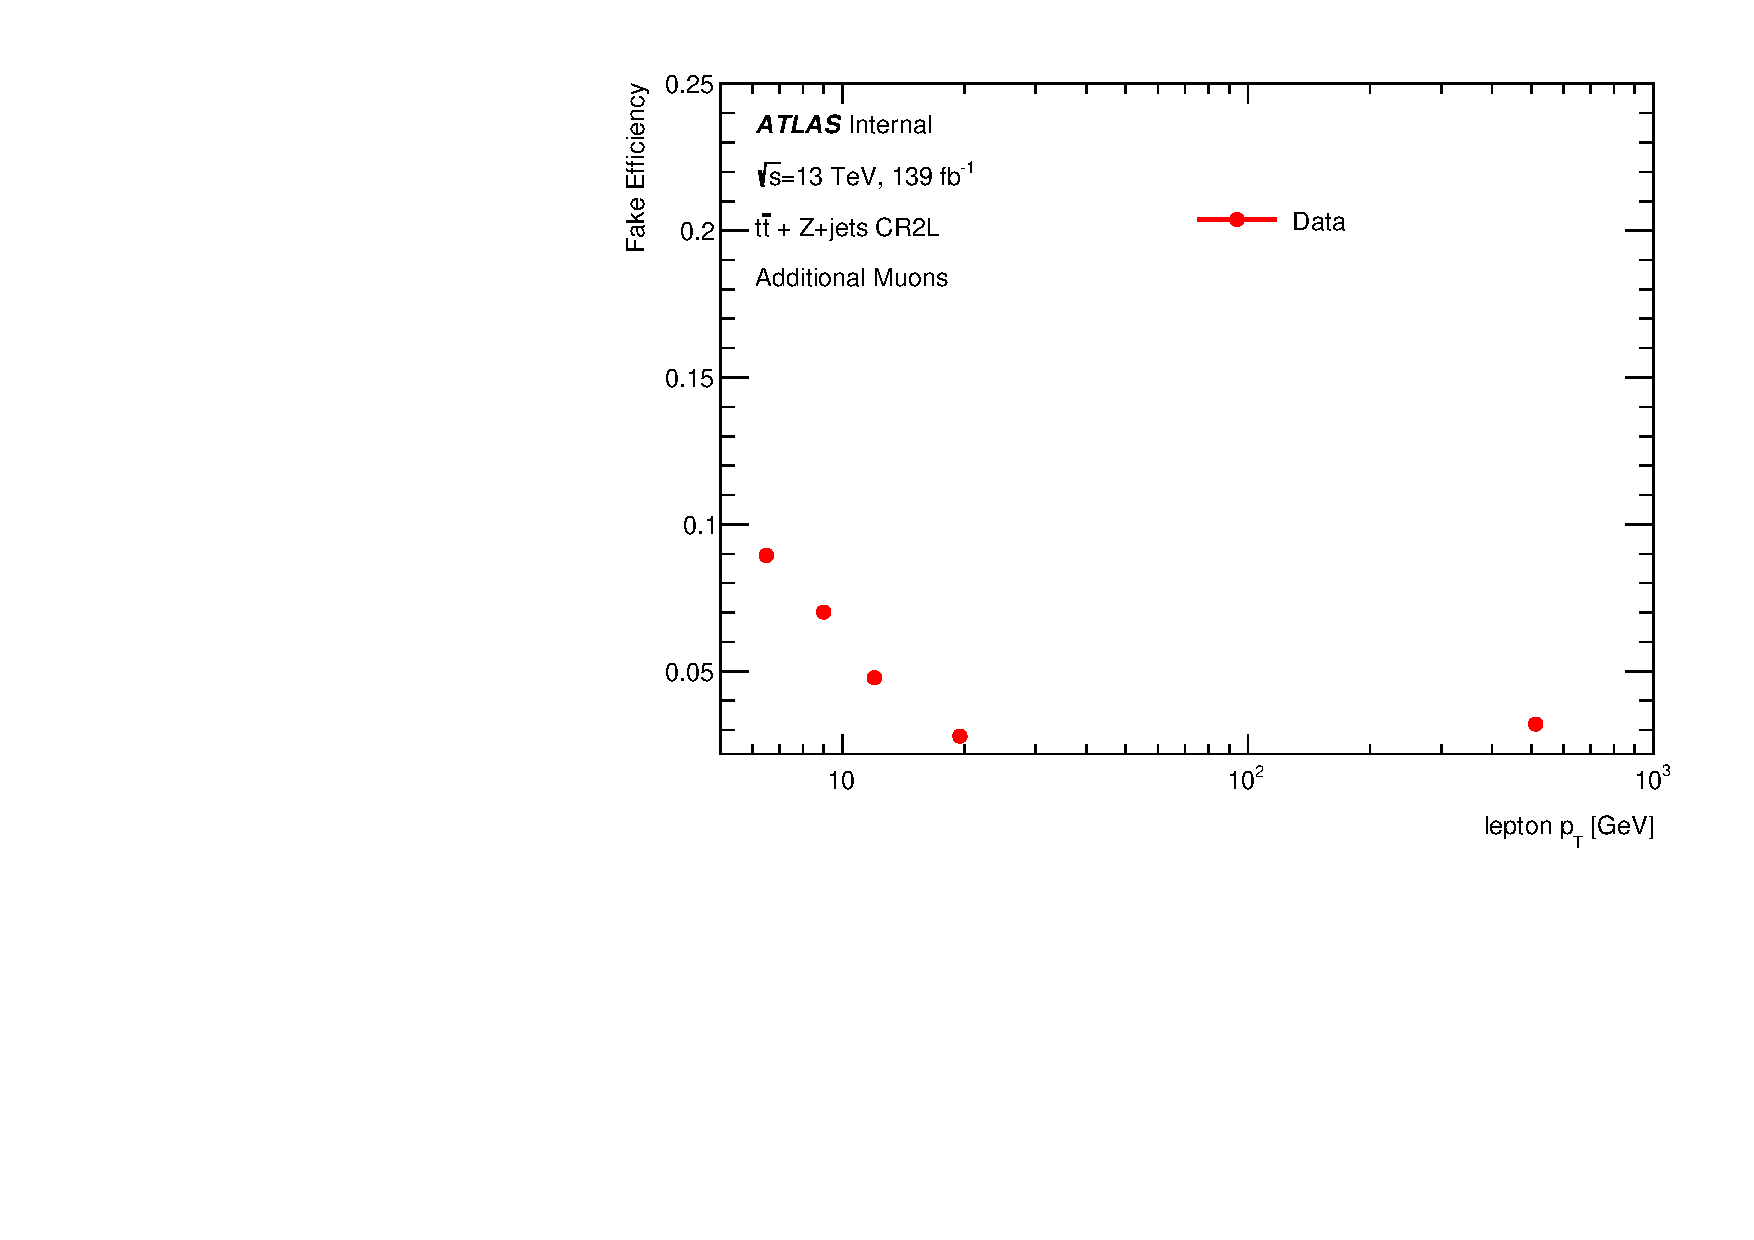
\includegraphics[width = 0.49\textwidth]{figures/Analysis/Background/Fake_Eff_Muon_pt_1D.pdf}
        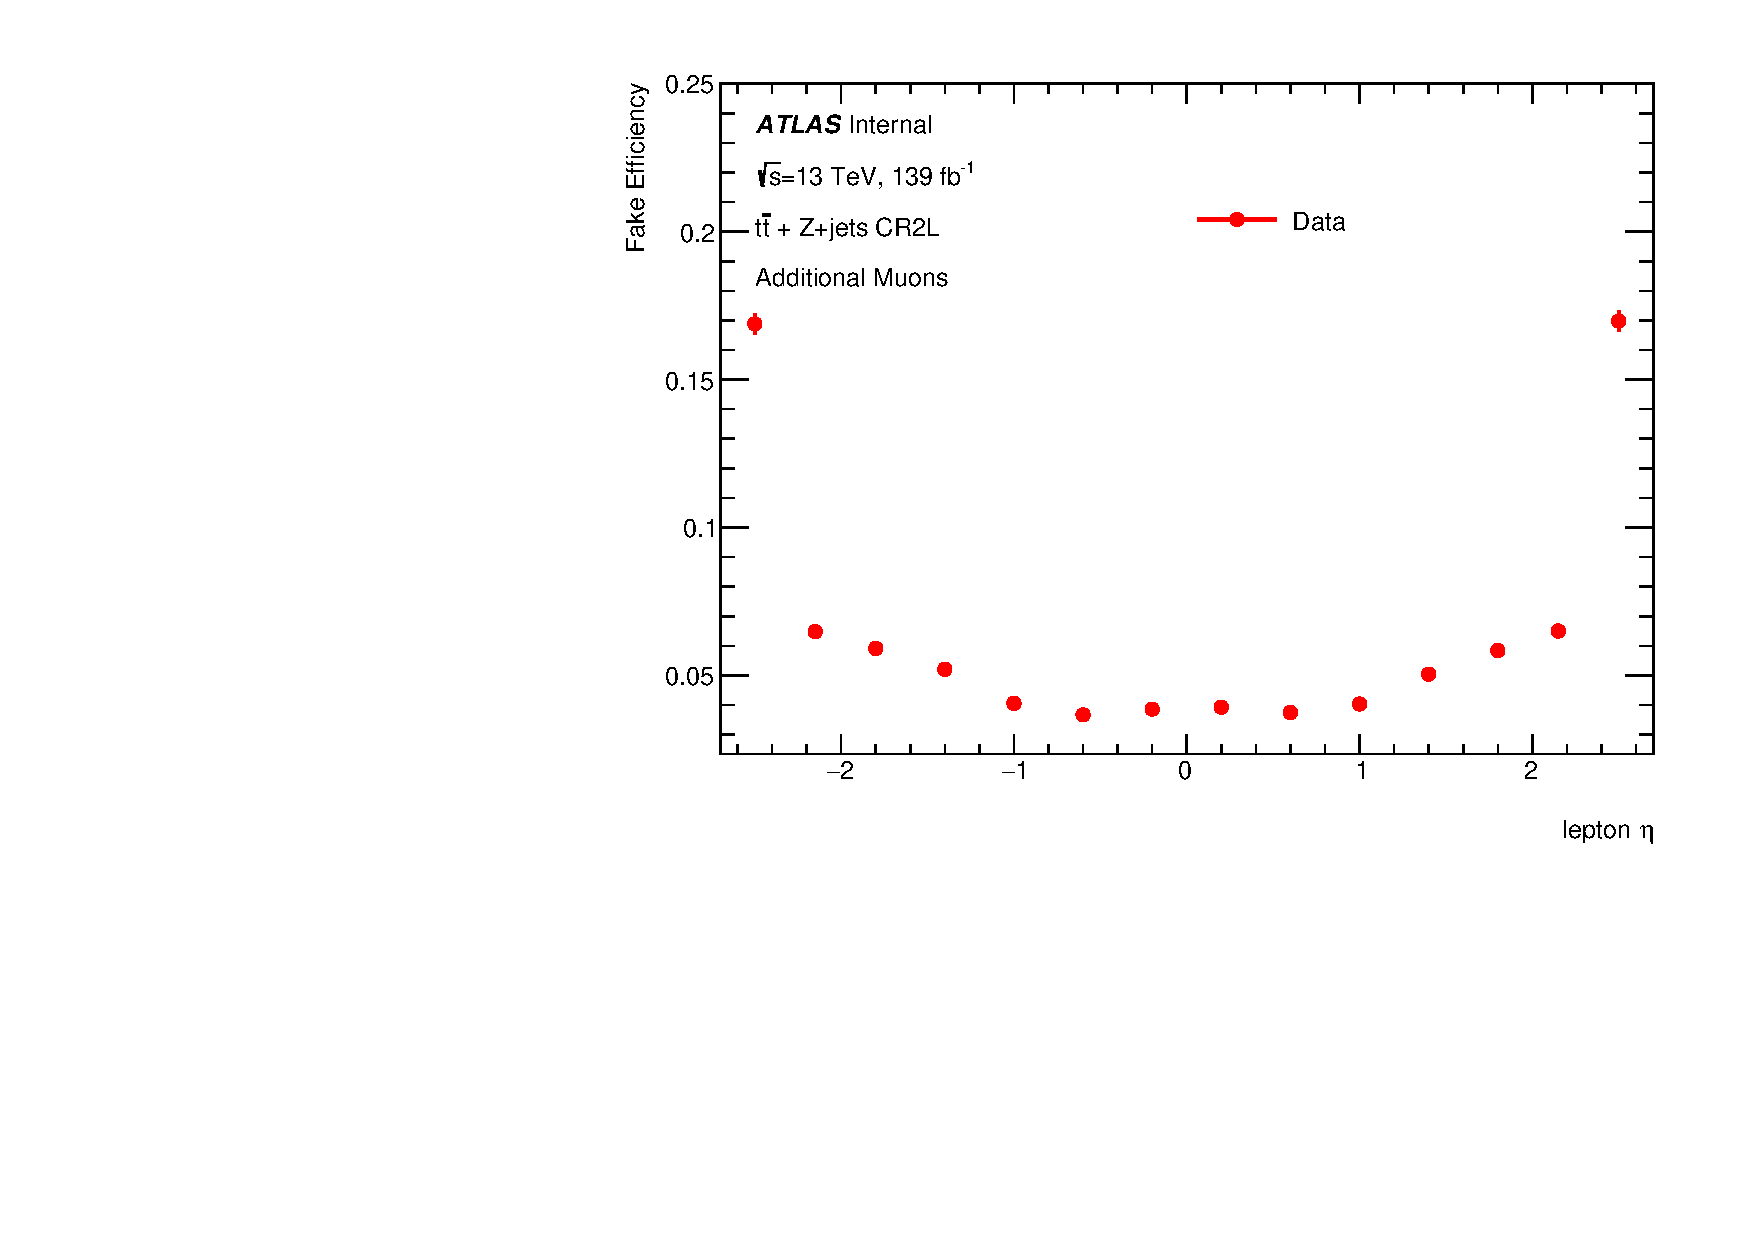
\includegraphics[width = 0.49\textwidth]{figures/Analysis/Background/Fake_Eff_Muon_eta_1D.pdf} \\
        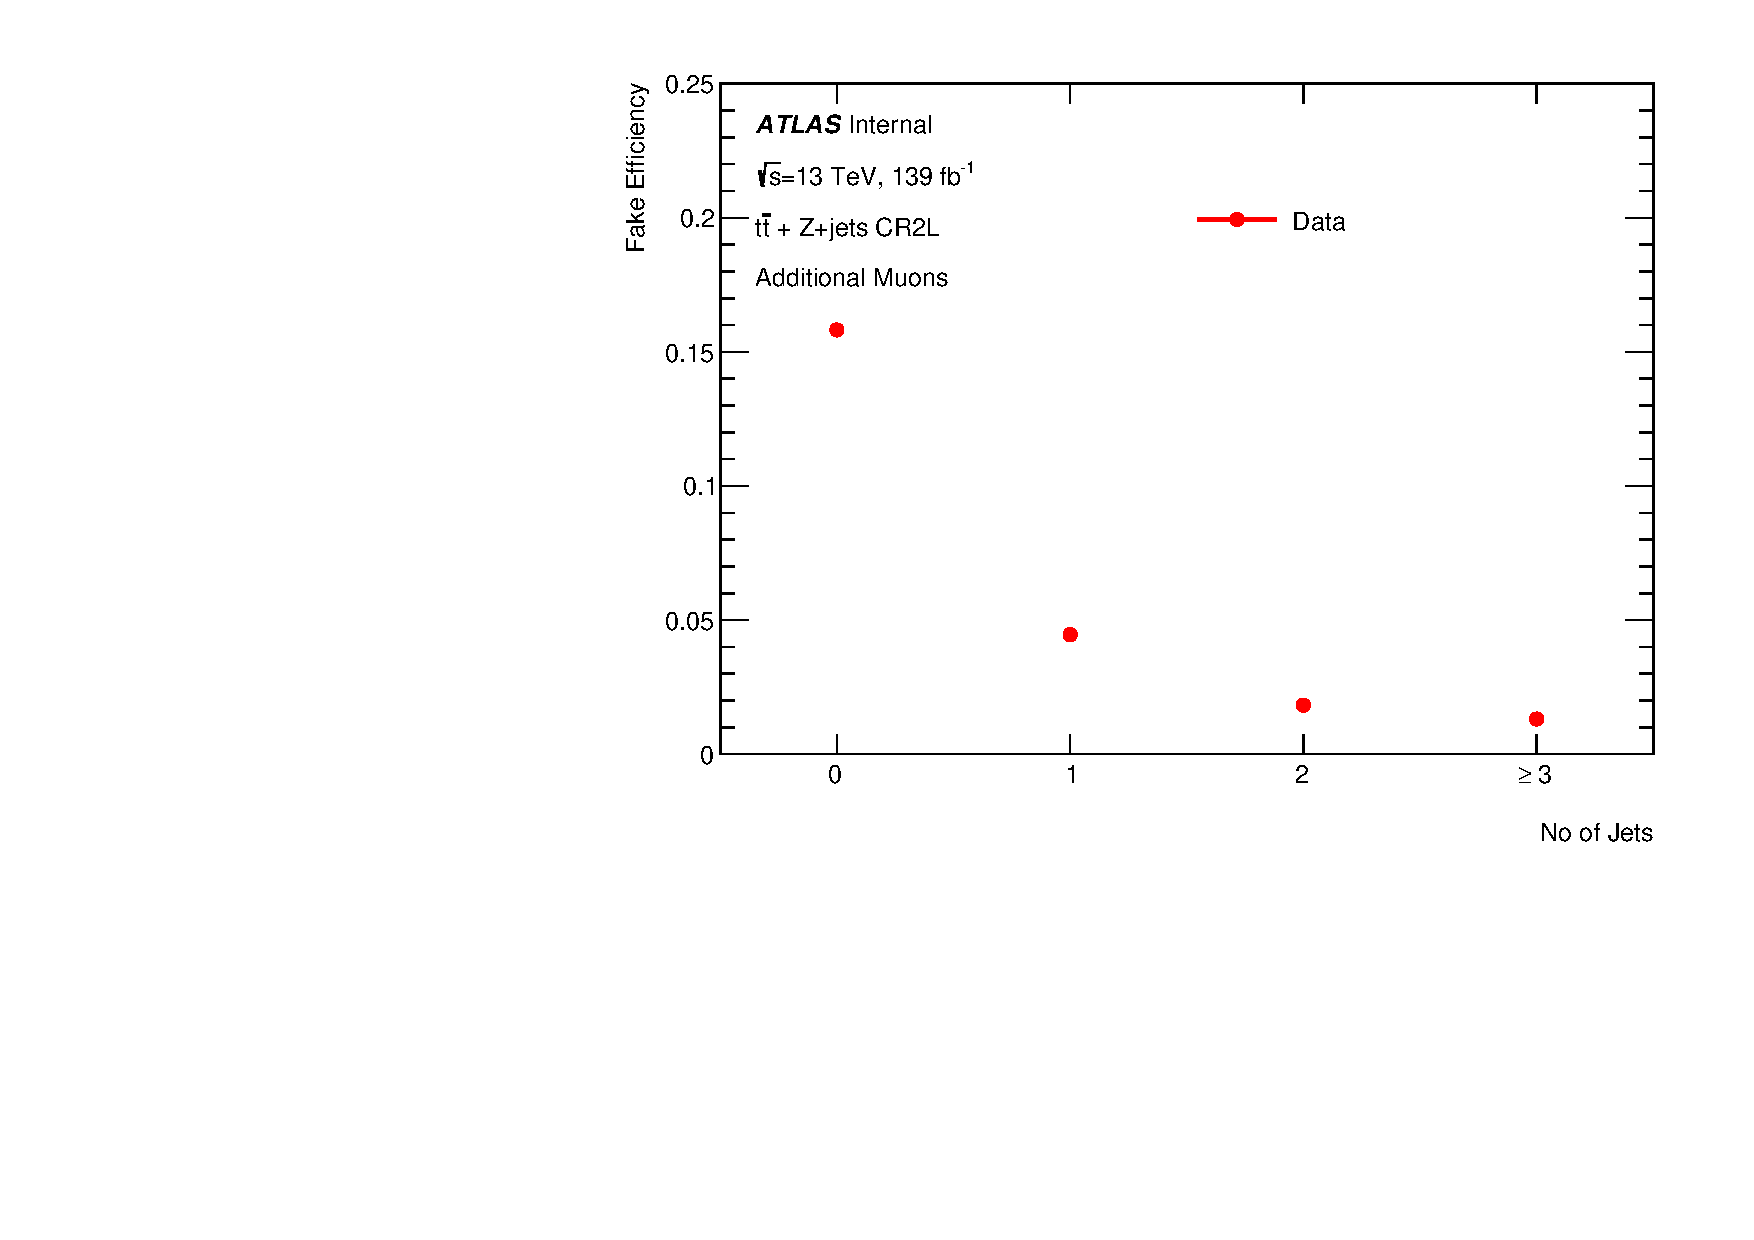
\includegraphics[width = 0.49\textwidth]{figures/Analysis/Background/Fake_Eff_Muon_jet_n_1D.pdf} 
        \end{center}
    \caption{Fake efficiency of fake muons measured in the combined control region from data as a function of its $p_{T}$, $\eta$, and $n_{jets}$. \label{fig:FakeEff_1D_Muon}}
\end{figure}

The final fake efficiencies in the data-driven fake background estimate are parametrized in three-dimensional distributions of $p_{T}$, $\eta$, and $n_{jets}$. Only two bins ($n_{jet}=0 ~\& ~ n_{jet} > 0$) are used for the number of jets to reduce statistical fluctuations. Figures \ref{fig:FakeEff_3D_Elec_njet0} and \ref{fig:FakeEff_3D_Elec_njet1} show the fake efficiency of an electron as a function of $p_{T} ~\&~ \eta$ for $n_{jet}=0 $ and $n_{jet}>0 $ bins, respectively. Similar distributions are shown in Figures \ref{fig:FakeEff_3D_Muon_njet0} and \ref{fig:FakeEff_3D_Muon_njet1} for muons.  

\begin{figure}[htb]
    \begin{center}
        \begin{subfigure}{.48\textwidth}
            \centering
            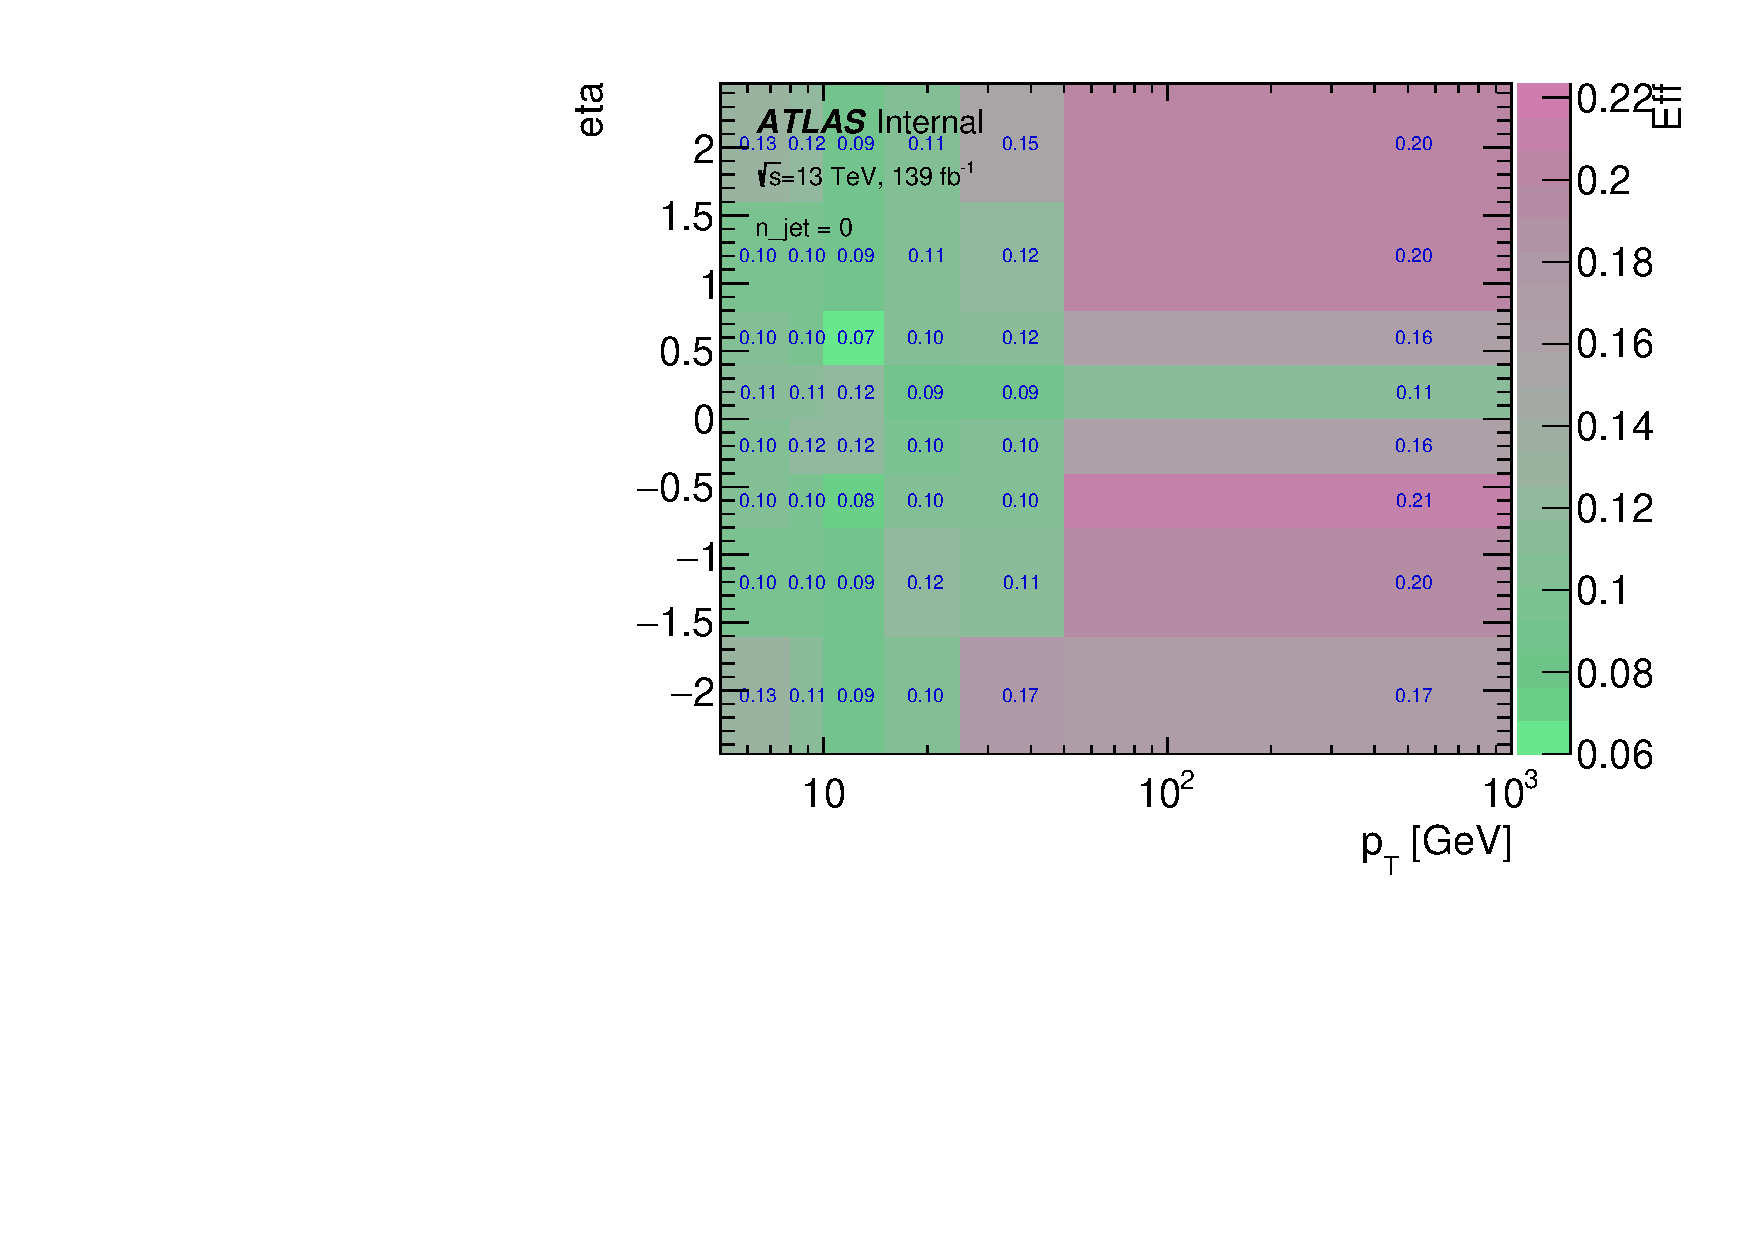
\includegraphics[width=.95\linewidth]{figures/Analysis/Background/njet0_FakeEfficiency3D_el_pt_eta.pdf}
            \caption{$n_{jet}=0$ events \label{fig:FakeEff_3D_Elec_njet0}}
        \end{subfigure}
        \begin{subfigure}{.48\textwidth}
            \centering
            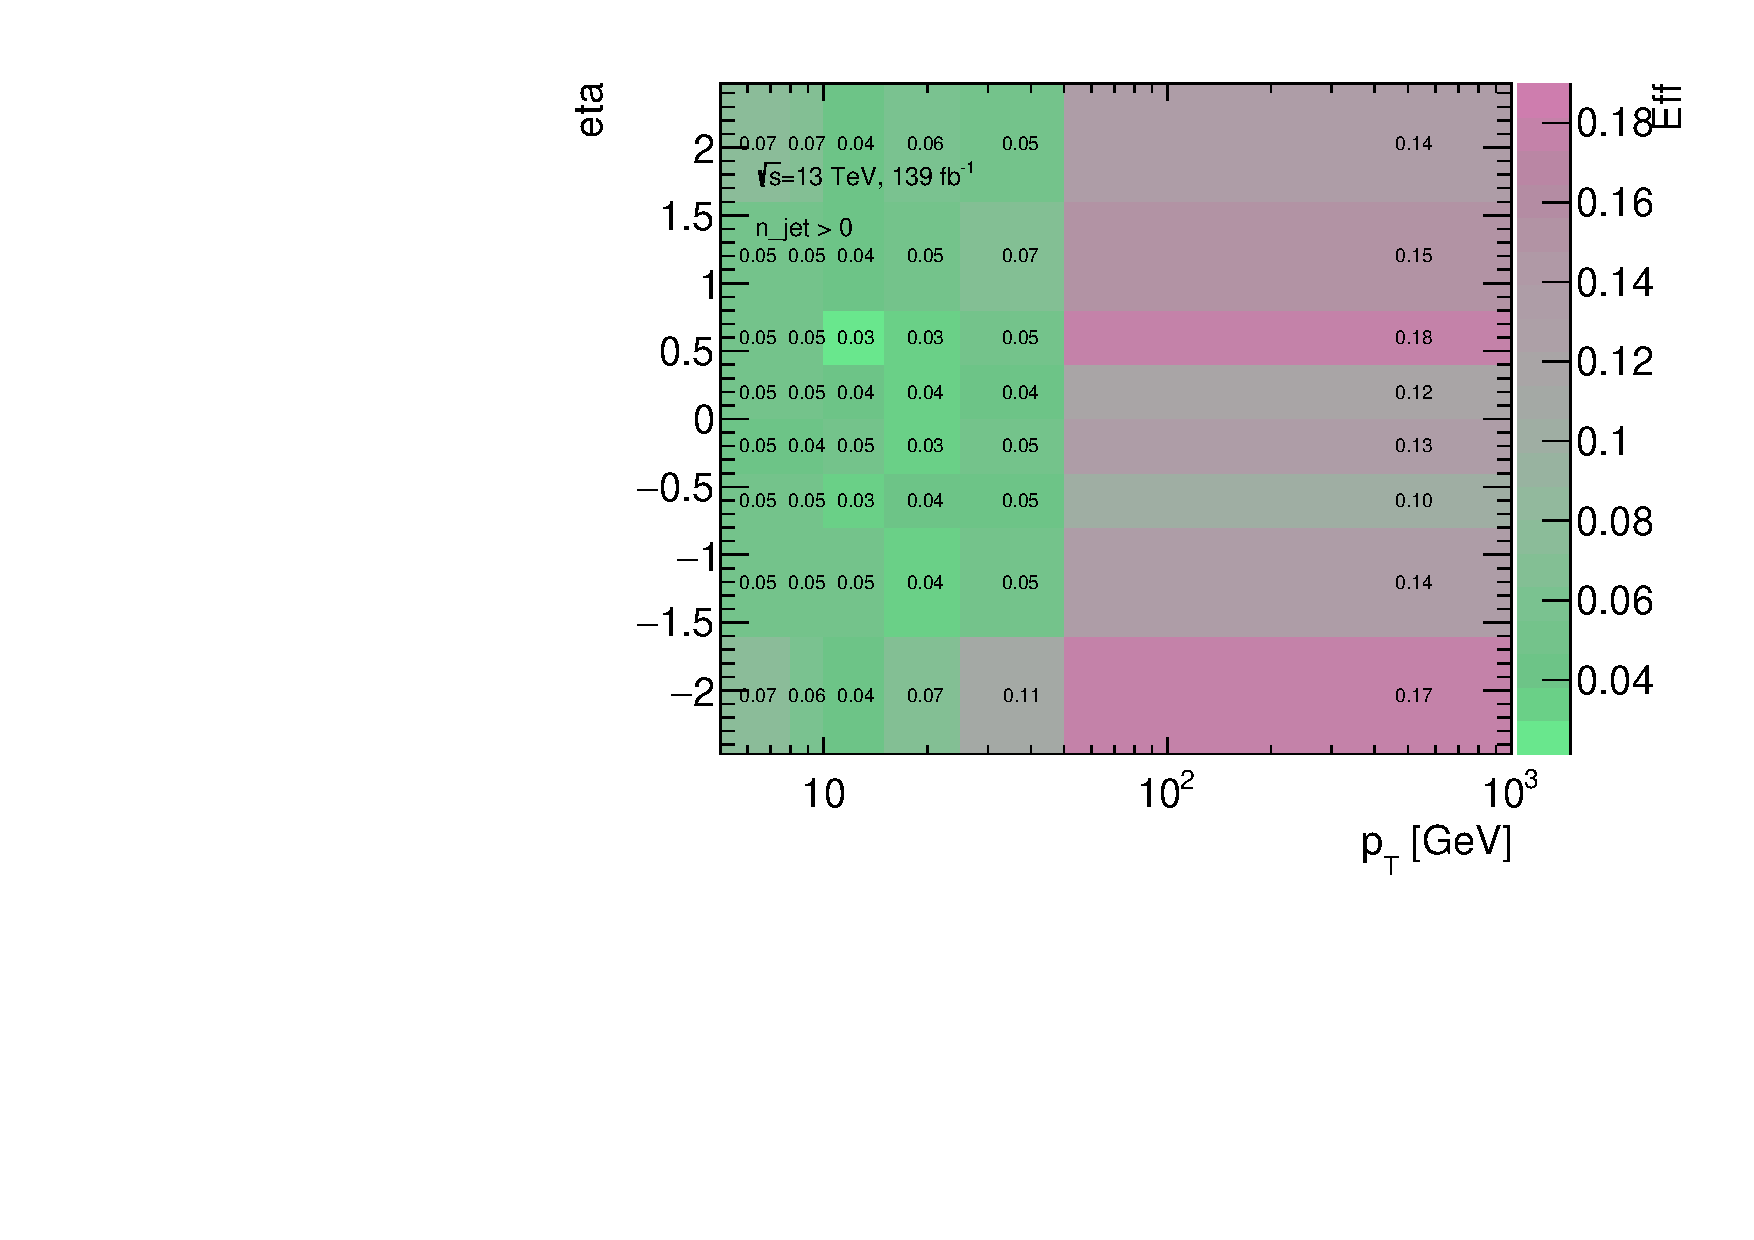
\includegraphics[width=.95\linewidth]{figures/Analysis/Background/njet1_FakeEfficiency3D_el_pt_eta.pdf}
            \caption{$n_{jet}>0$ events \label{fig:FakeEff_3D_Elec_njet1}}
        \end{subfigure}
    \end{center}
    \caption{Fake efficiency of fake electrons measured in the combined control region from data as a function of its $p_{T}$, and $\eta$ in two slices of $n_{jets}$. \label{fig:ElecFakeEff}}
\end{figure}

\begin{figure}[htb]
        \begin{center}
        \begin{subfigure}{.48\textwidth}
            \centering
            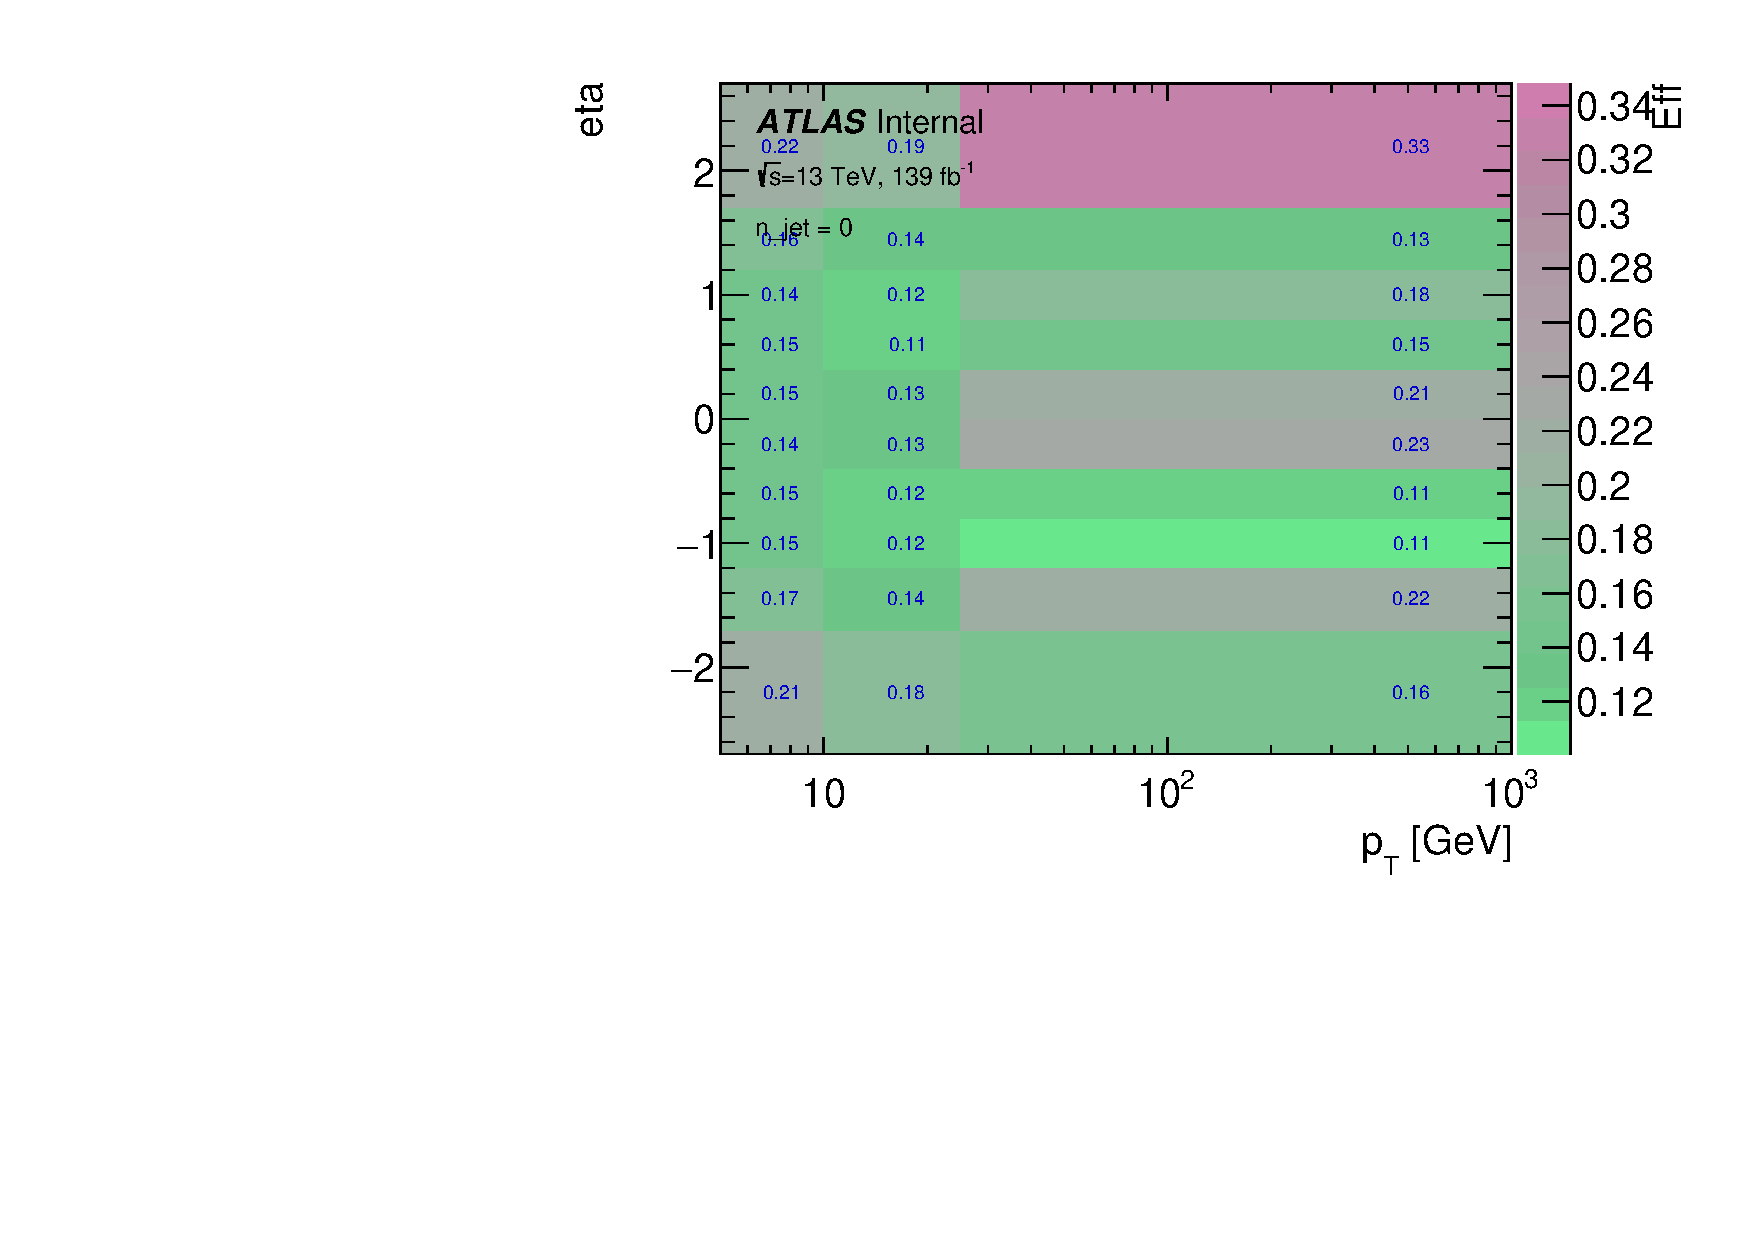
\includegraphics[width=.95\linewidth]{figures/Analysis/Background/njet0_FakeEfficiency3D_mu_pt_eta.pdf}
            \caption{$n_{jet}=0$ events \label{fig:FakeEff_3D_Muon_njet0}}
        \end{subfigure}
        \begin{subfigure}{.48\textwidth}
            \centering
            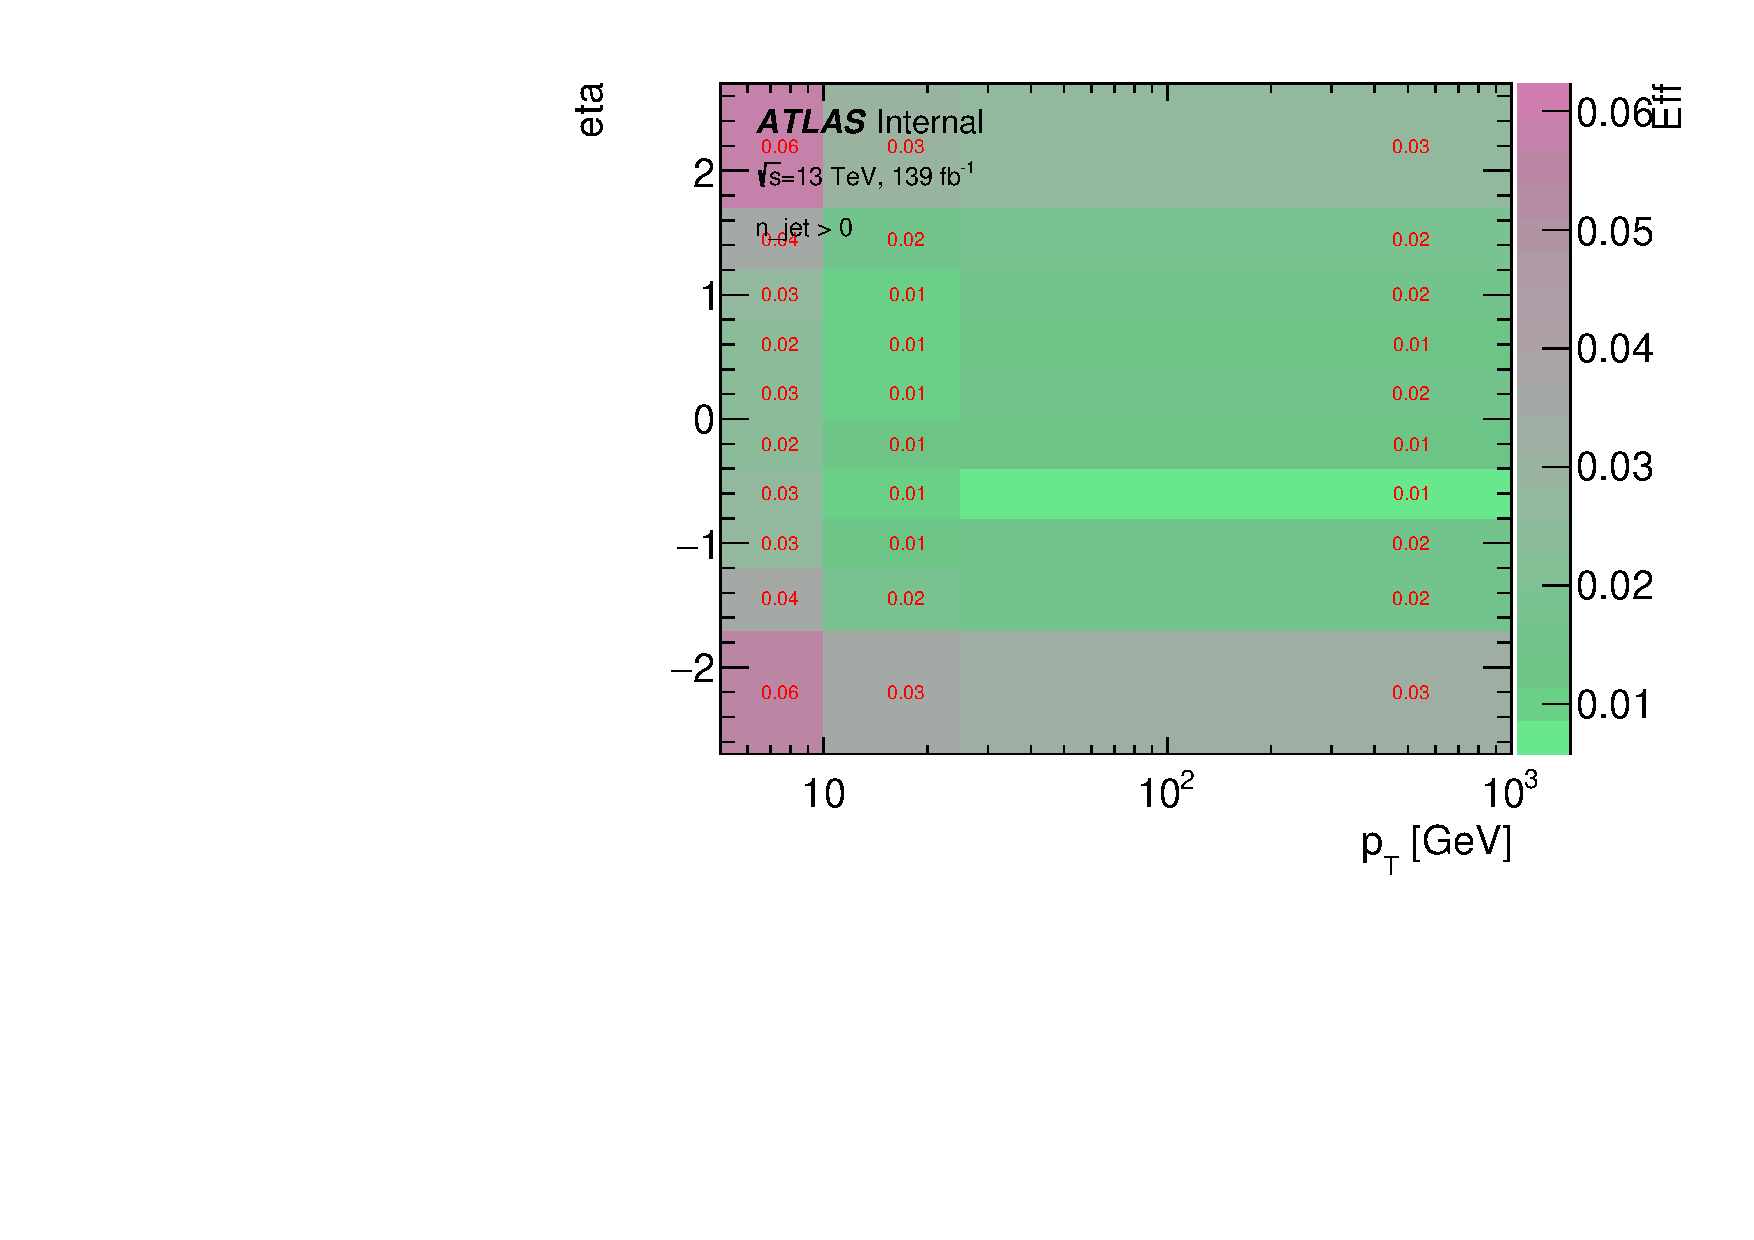
\includegraphics[width=.95\linewidth]{figures/Analysis/Background/njet1_FakeEfficiency3D_mu_pt_eta.pdf}
            \caption{$n_{jet}>0$ events \label{fig:FakeEff_3D_Muon_njet1}}
        \end{subfigure}
        \end{center}
    \caption{Fake efficiency of fake muons measured in the combined control region from data as a function of its $p_{T}$, and $\eta$ in two slices of $n_{jets}$. \label{fig:MuonFakeEff}}
\end{figure}

The fake efficiency distributions' binomial errors are propagated as the statistical uncertainties on the fake estimate. The subtracted prompt component of equation \ref{eq:fakeff} is estimated using MC predictions. As discussed in Section \ref{sec:Pheno}, the prediction relies on the PDF, the energy-dependent QCD factorization and renormalization scale, and the strong coupling constant $(\alpha_{S})$. Therefore, the theory uncertainties on these three parameters are propagated as systematic uncertainties of the fake efficiency. 

For each theory uncertainty, a variation-applied fake efficiency is evaluated by separately varying the numerator and denominator of the fake efficiency equation \ref{eq:fakeff}. The difference between the variation-applied fake efficiency and the nominal fake efficiency is considered systematic uncertainty. Figures \ref{fig:FakeEffUnc_3D_Electron} and \ref{fig:FakeEffUnc_3D_Muon} show the statistical and systematic uncertainties on the fake efficiencies for electrons and muons, respectively, as a function of their $p_{T},~\eta,~\&~n_{jets}$ calculated in the combined control region. For both electrons and muons, the statistical uncertainty is dominant.

\begin{figure}[htb]
    \begin{center}
    \begin{subfigure}{.48\textwidth}
        \centering
        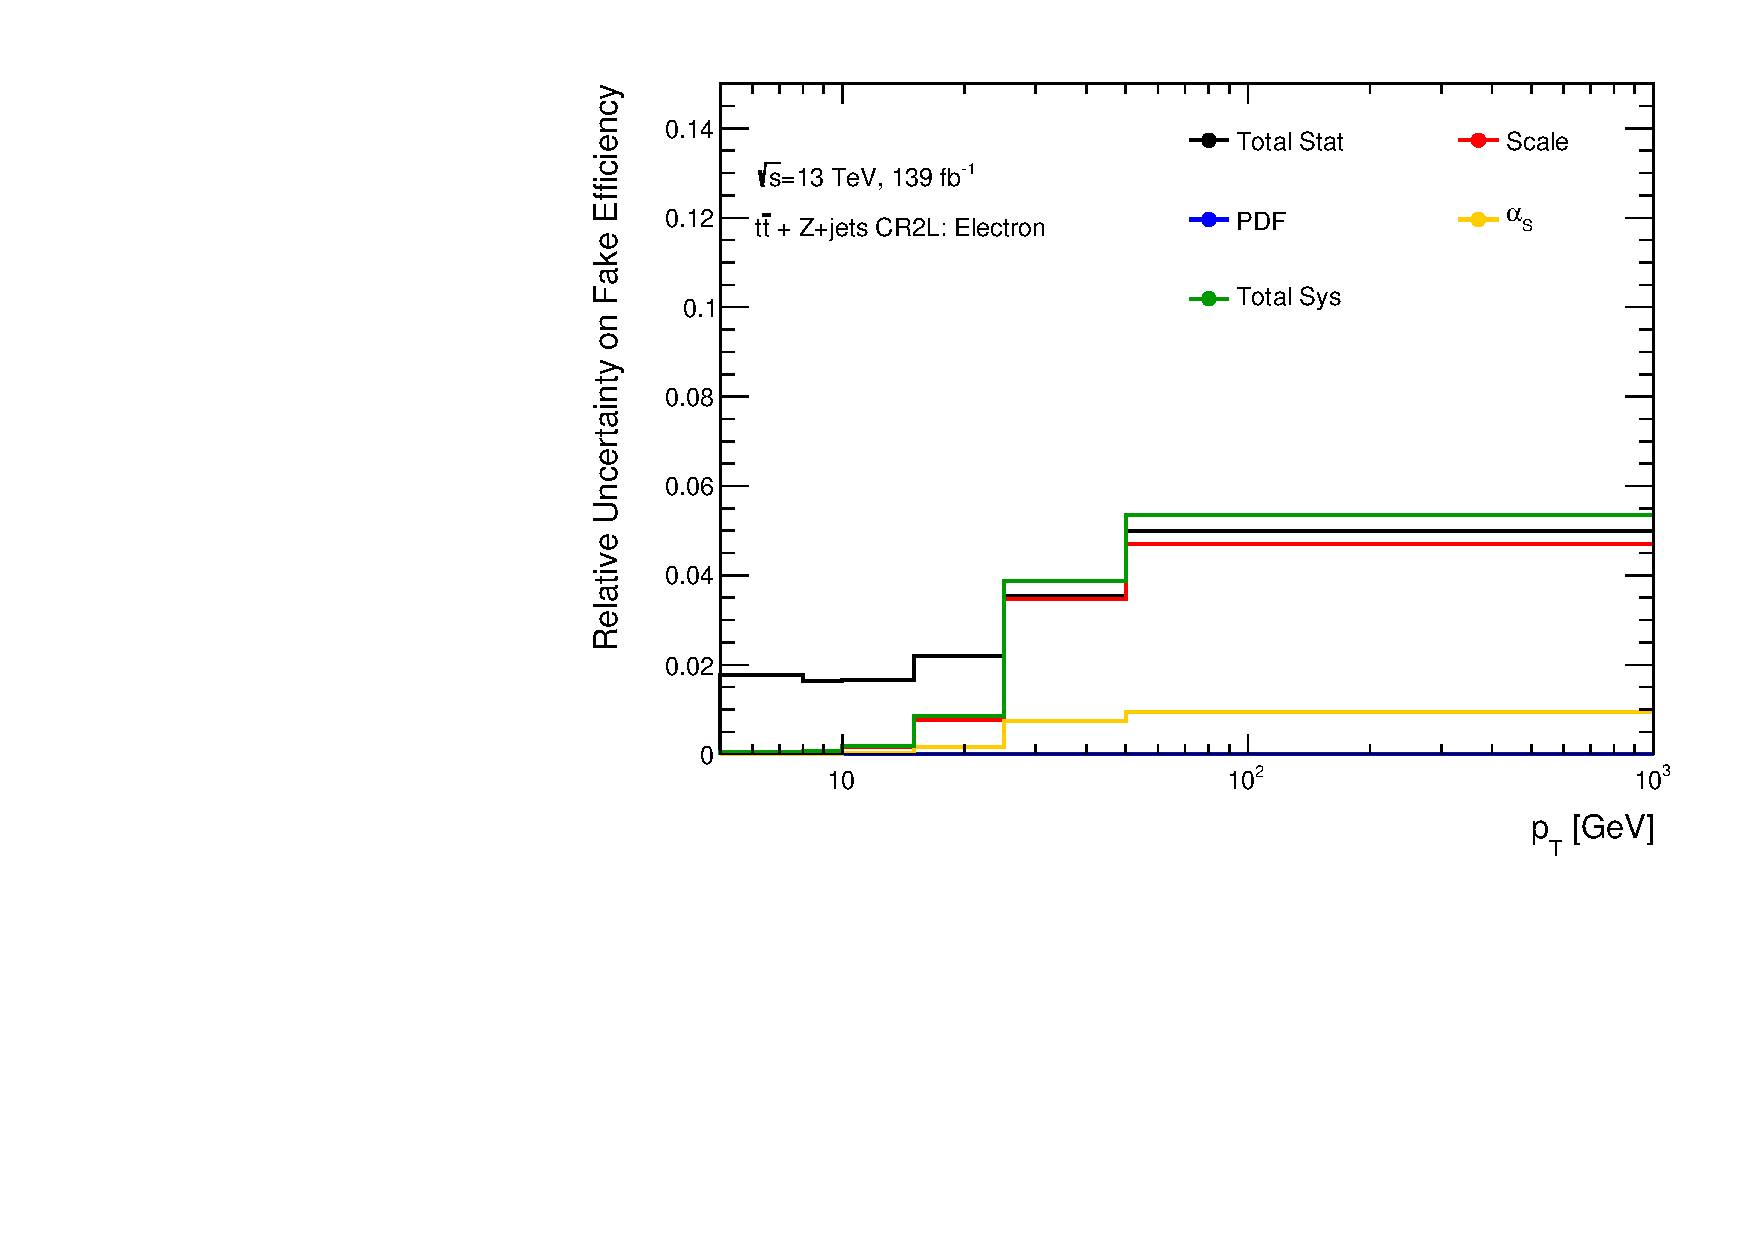
\includegraphics[width=.95\linewidth]{figures/Analysis/Background/SystematicUncertainties3D_Electron_pT.pdf}
        \caption{$p_{T}$ \label{fig:FakeUnc_pt_e}}
    \end{subfigure}
    \begin{subfigure}{.48\textwidth}
        \centering
        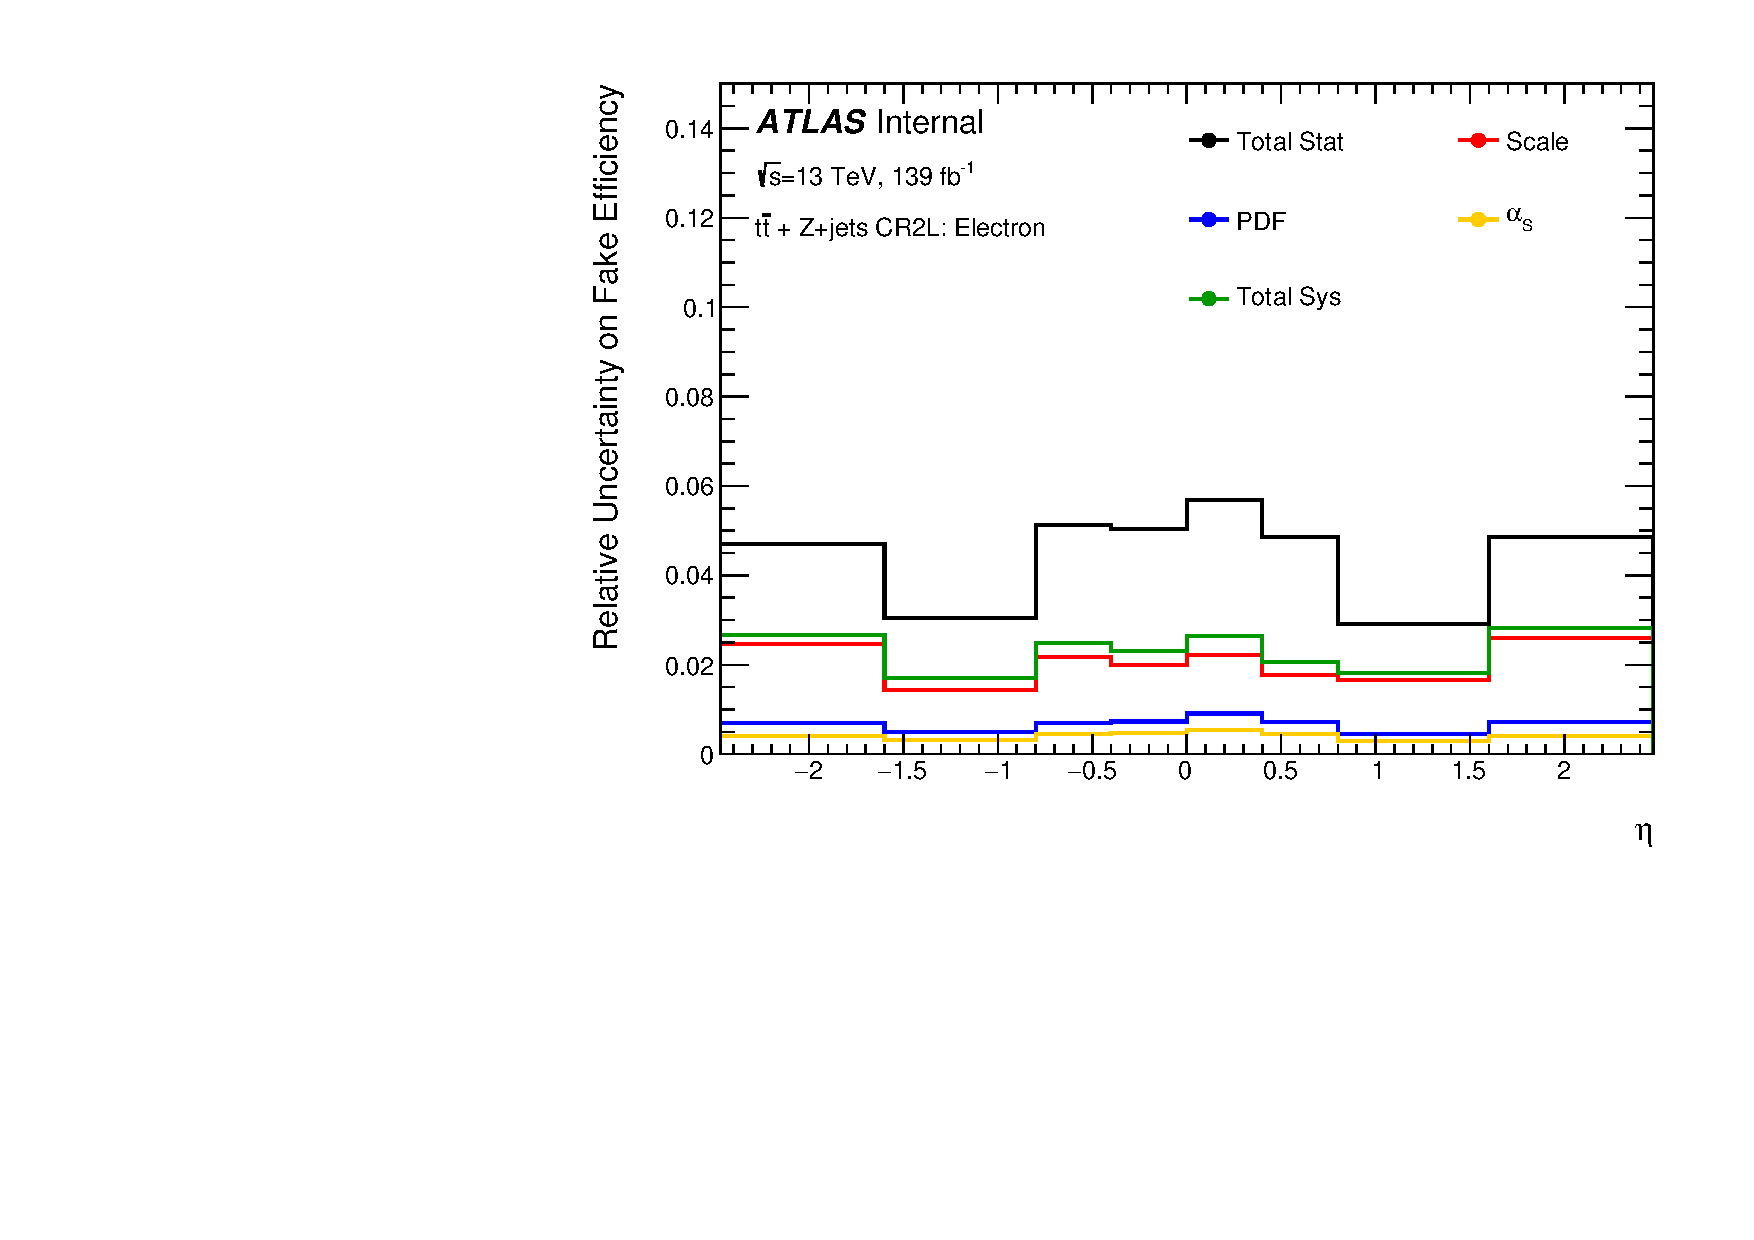
\includegraphics[width=.95\linewidth]{figures/Analysis/Background/SystematicUncertainties3D_Electron_eta.pdf}
        \caption{$\eta$ \label{fig:FakeUnc_eta_e}}
    \end{subfigure}\\
    \begin{subfigure}{.48\textwidth}
        \centering
        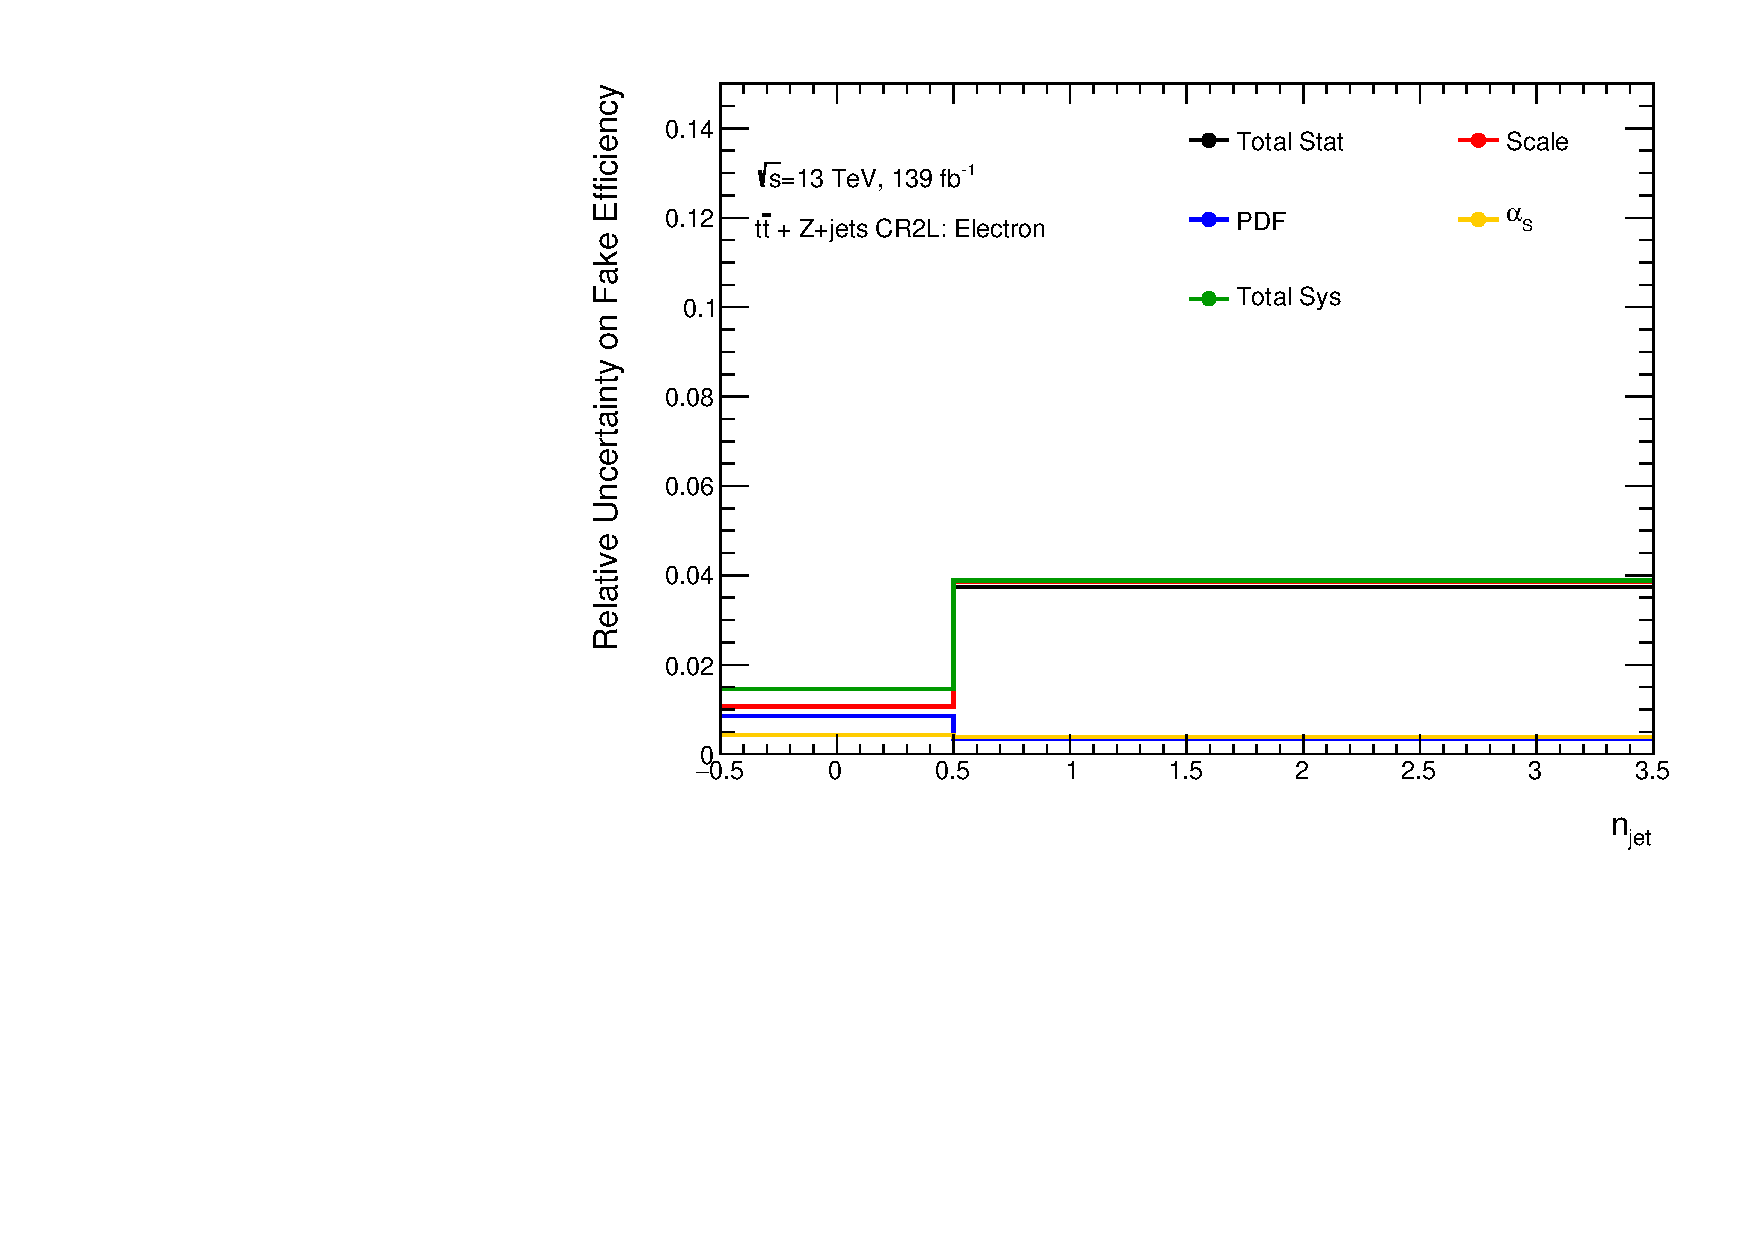
\includegraphics[width=.95\linewidth]{figures/Analysis/Background/SystematicUncertainties3D_Electron_njet.pdf}
        \caption{$n_{jet}$ \label{fig:FakeUnc_njet_e}}
    \end{subfigure}
    \end{center}
\caption{Uncertainties on the fake efficiency of the fake electrons measured in the combined control region from data as a function of their $p_{T}$, $\eta$, and $n_{jets}$. \label{fig:FakeEffUnc_3D_Electron}}
\end{figure}

\begin{figure}[htb]
    \begin{center}
    \begin{subfigure}{.48\textwidth}
        \centering
        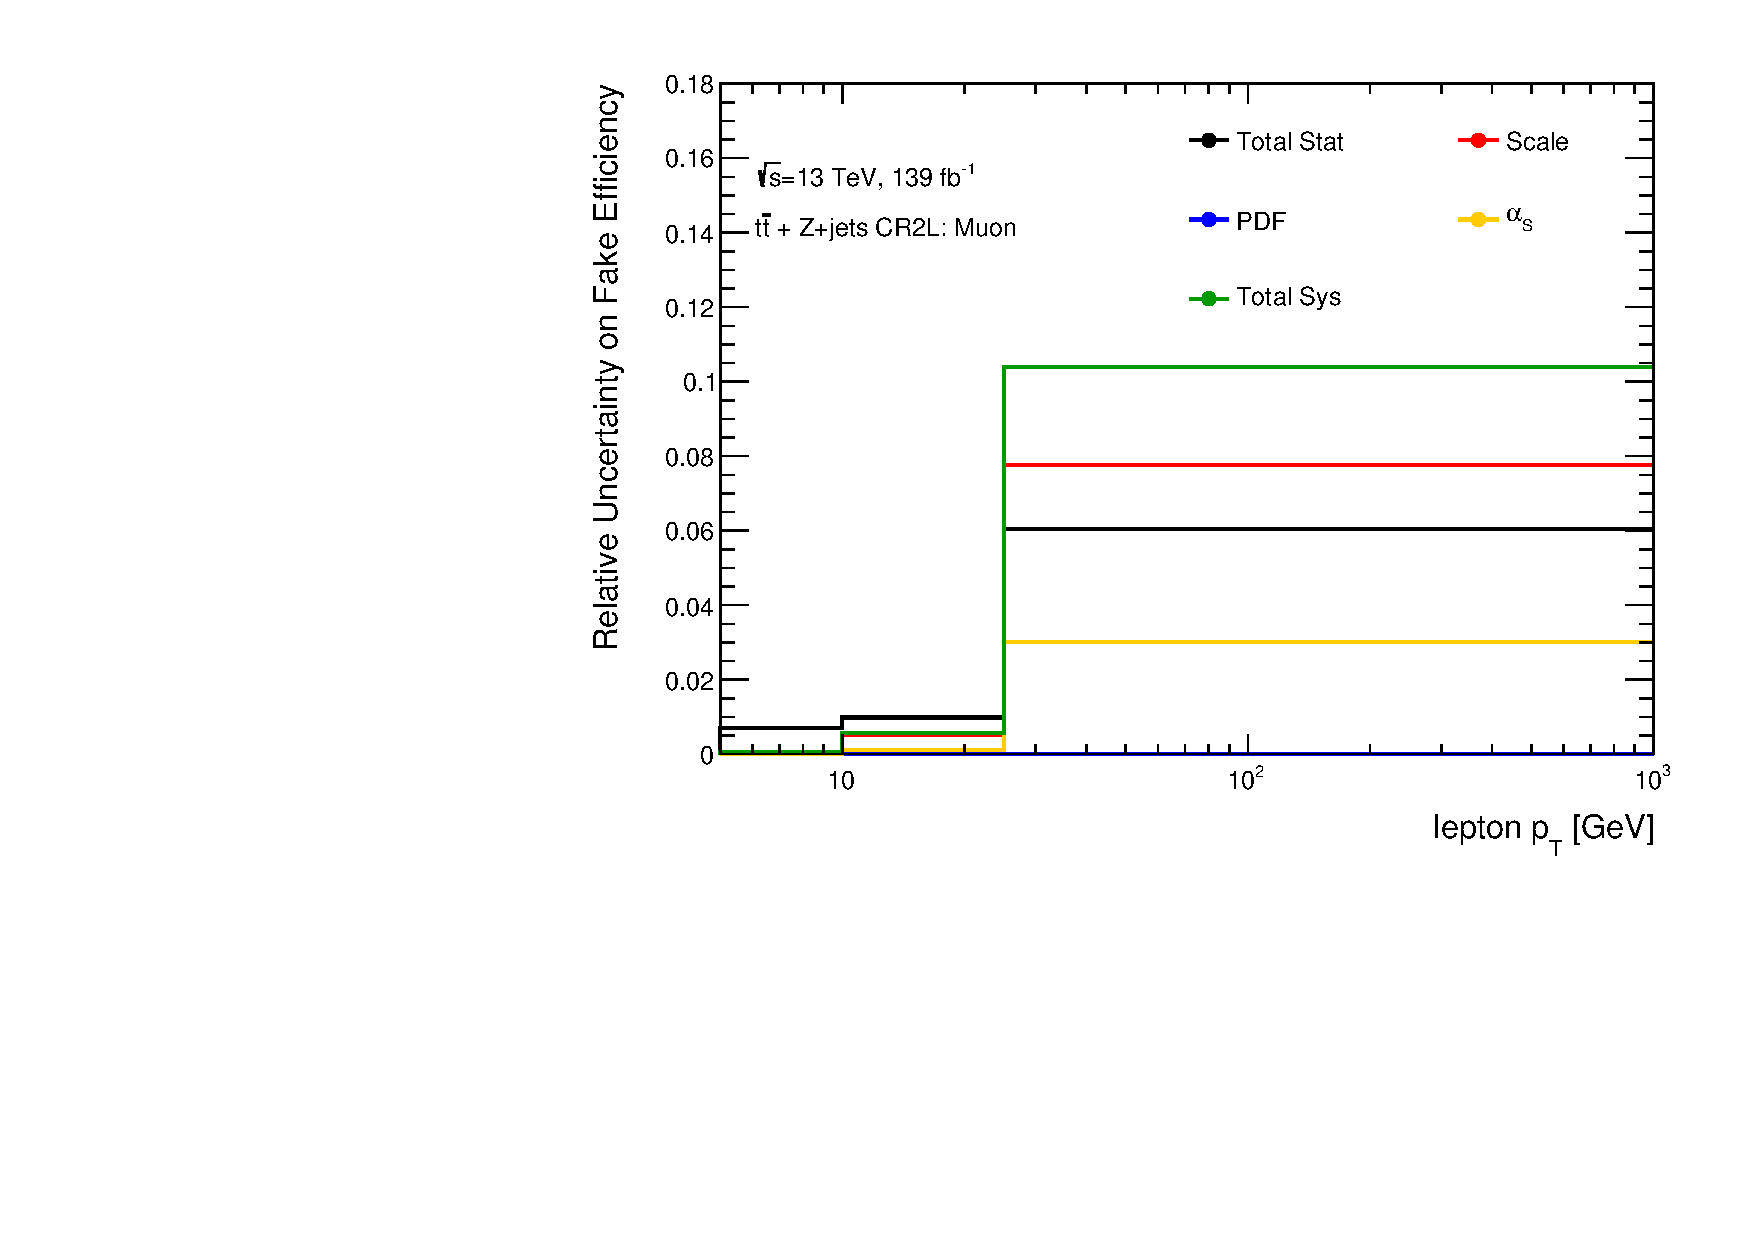
\includegraphics[width=.95\linewidth]{figures/Analysis/Background/SystematicUncertainties3D_Muon_pT.pdf}
        \caption{$p_{T}$ \label{fig:FakeUnc_pt_mu}}
    \end{subfigure}
    \begin{subfigure}{.48\textwidth}
        \centering
        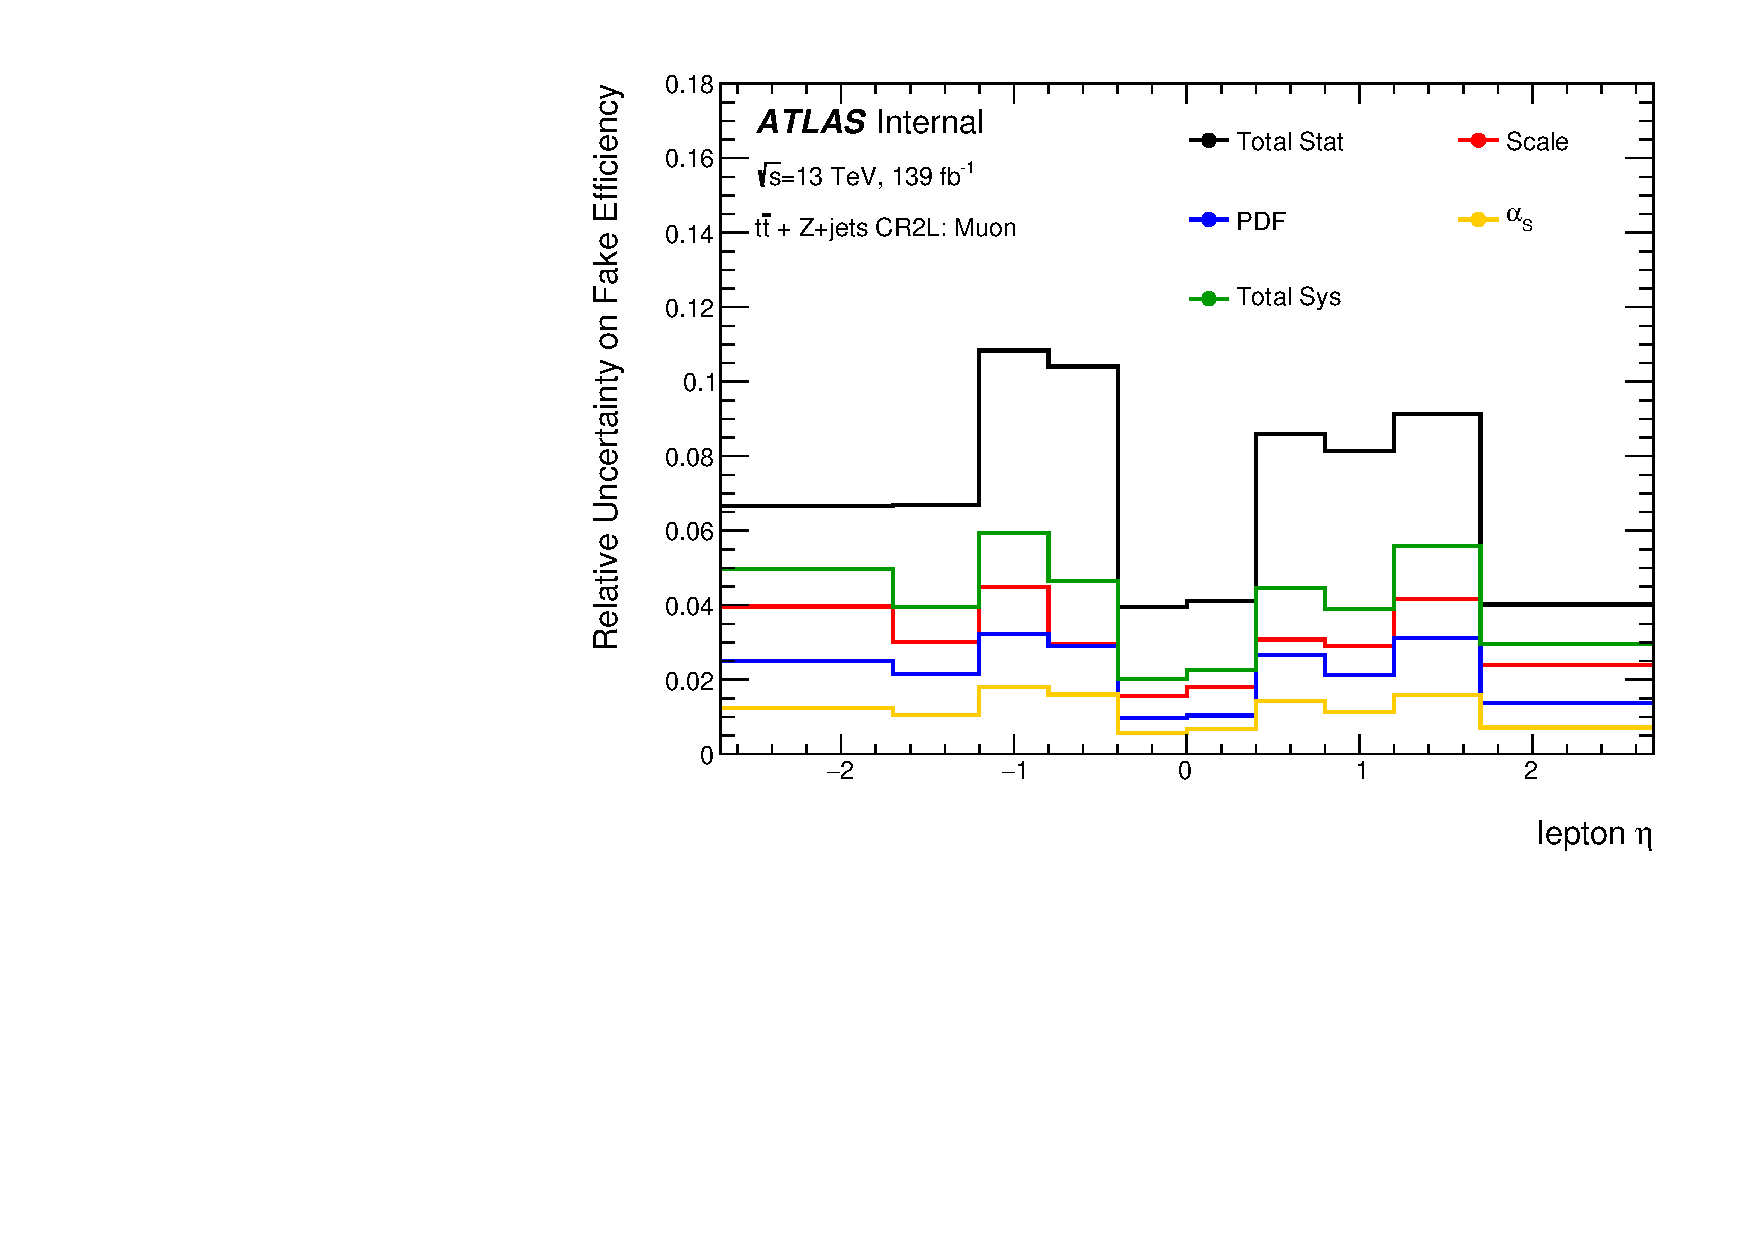
\includegraphics[width=.95\linewidth]{figures/Analysis/Background/SystematicUncertainties3D_Muon_eta.pdf}
        \caption{$\eta$ \label{fig:FakeUnc_eta_mu}}
    \end{subfigure}\\
    \begin{subfigure}{.48\textwidth}
        \centering
        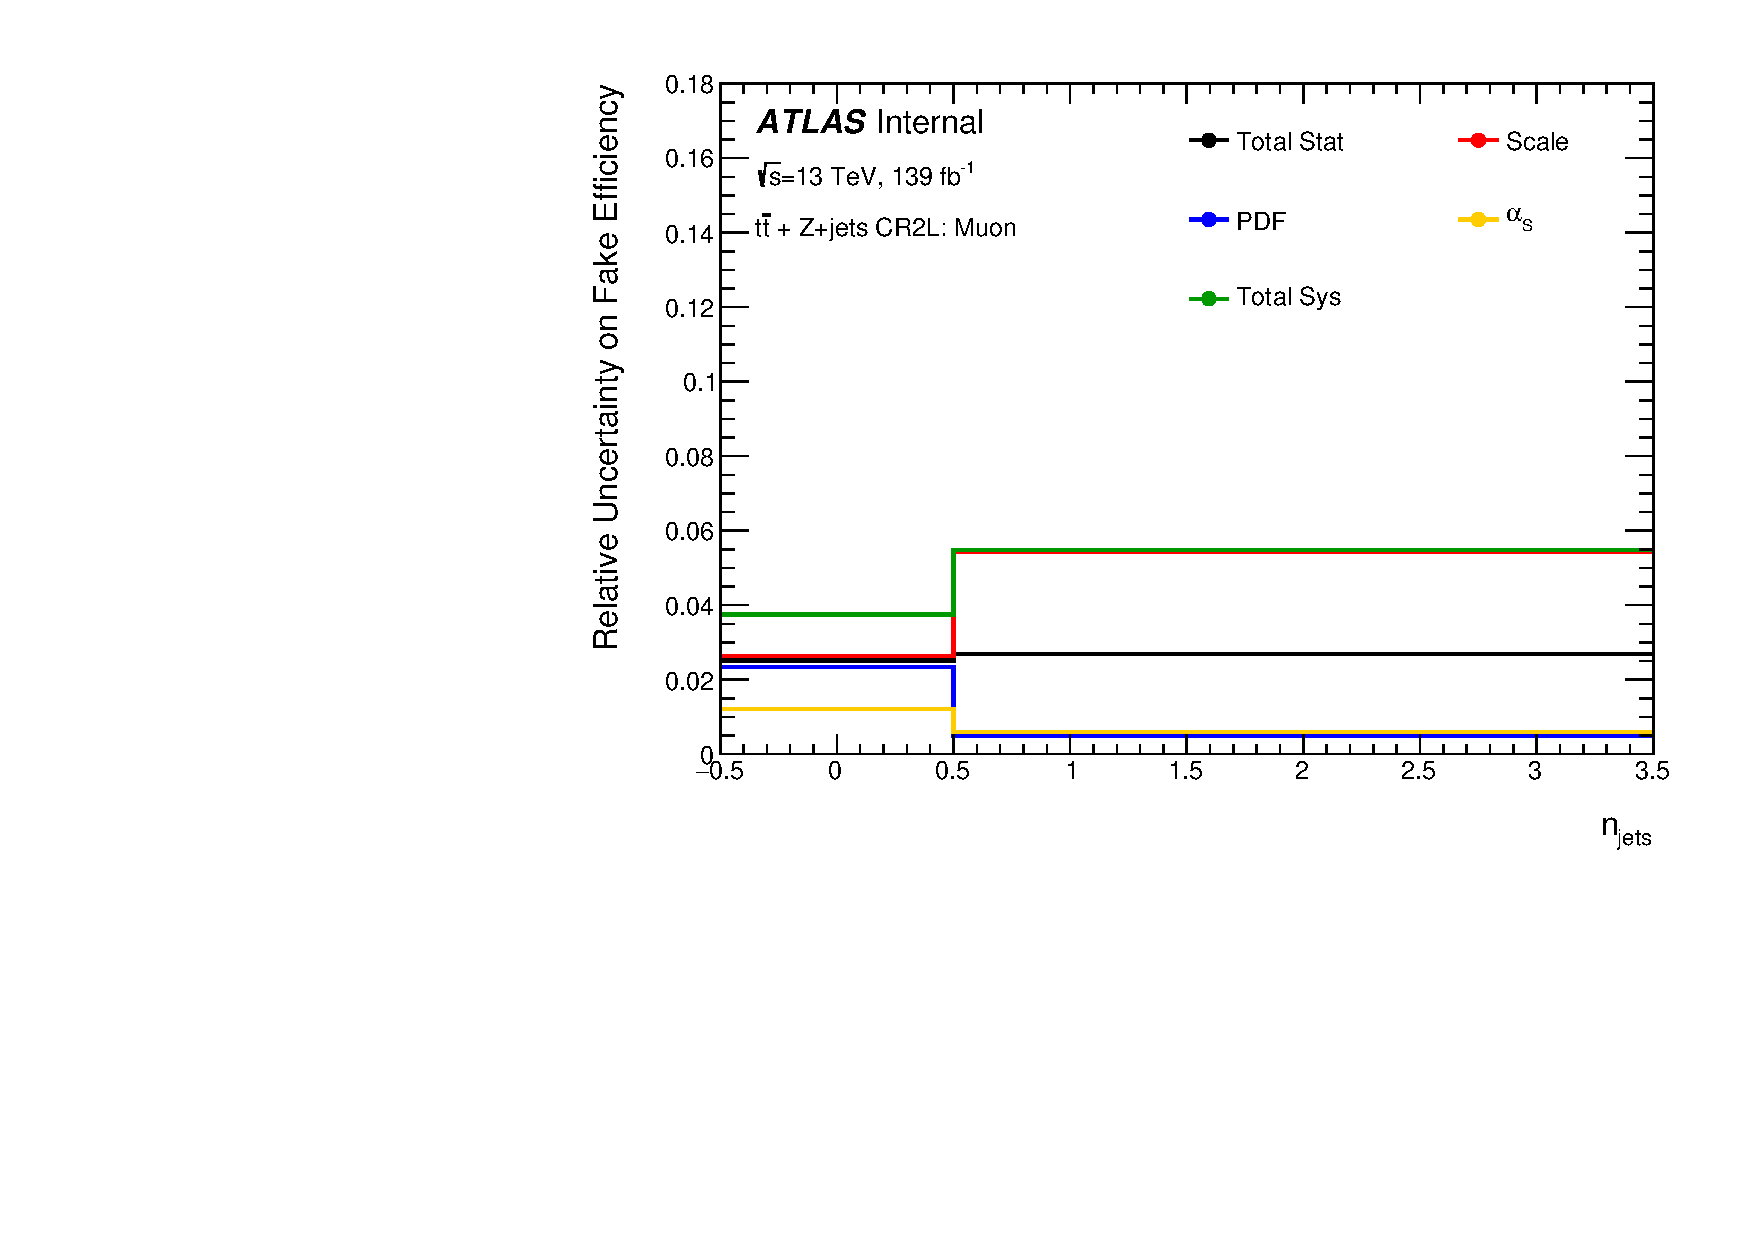
\includegraphics[width=.95\linewidth]{figures/Analysis/Background/SystematicUncertainties3D_Muon_njet.pdf}
        \caption{$n_{jet}$ \label{fig:FakeUnc_njet_mu}}
    \end{subfigure}
    \end{center}
\caption{Uncertainties on the fake efficiency of the fake muons measured in the combined control region from data as a function of their $p_{T}$, $\eta$, and $n_{jets}$. \label{fig:FakeEffUnc_3D_Muon}}
\end{figure}

\subsubsection{Method Validation}
\label{subsubsec:Validation}
Before implementing the fake-factor method to estimate the fake background in the signal region, the method is validated in two separate validation regions
\begin{enumerate}
    \item{ Different-flavor validation region (VRDF): one pair in the quadruplet must have two different-flavor leptons.}
    \item{ Same-charge validation region (VRSC): one pair in the quadruplet must have two same-charge leptons.}
\end{enumerate}

The low statistics in both regions result from requiring one of the pairs in the quadruplet to be either same-charge or different-flavor. Therefore, only signal quadruplets are required in the validation regions events without any dijet requirement. The validation regions' quadruplets are formed by requiring the same kinematic criteria as that of the signal region discussed in Section \ref{sec:EventSel}. The trigger requirement, object selection, and overlap removal are identical to the signal region. Additionally, events in the VRDF are required not to have any b-tagged jet to reduce the contribution from $ttZ$ processes. Reducing the $ttZ$ component further reduces the significant modeling uncertainties related to the $ttZ$ process.

By imposing either a same-charge or a different-flavor lepton pair, the event yield in validation regions is dominated by events where at least one lepton in the quadruplet is a non-prompt-signal lepton known as the fake background in the signal region. The events also originate from other physics processes, such as $qqZZ$, $qqZZjj$, $ggZZ$, $ttZ$, and $VVV$ whose contribution is predicted by the same MC generators as that of the signal region.

Figures \ref{fig:VRDF_Elec_NonPromptComp} and \ref{fig:VRDF_Muon_NonPromptComp} show the non-prompt composition in the different flavor validation regions for non-prompt electrons and muons, respectively. Similarly, Figures \ref{fig:VRSC_Elec_NonPromptComp} and \ref{fig:VRSC_Muon_NonPromptComp} show the fake composition of the non-prompt electrons and muons, respectively, in the same-charge validation region. The non-prompt compositions in the two validation regions are different from that of the signal region shown in Figure \ref{fig:NonPromptLepSRDijet} or that of the background control regions composition shown in Figures \ref{fig:FakeCompositionCR2LElectron} and \ref{fig:FakeCompositionCR2LMuon}. Therefore, to validate the fake background estimation strategy, it is imperative to observe a good correspondence between data and a combination of the total MC prediction with the fake background yield in both validation regions.

\begin{figure}[htb]
    \centering
    \begin{subfigure}{.48\textwidth}
        \centering
        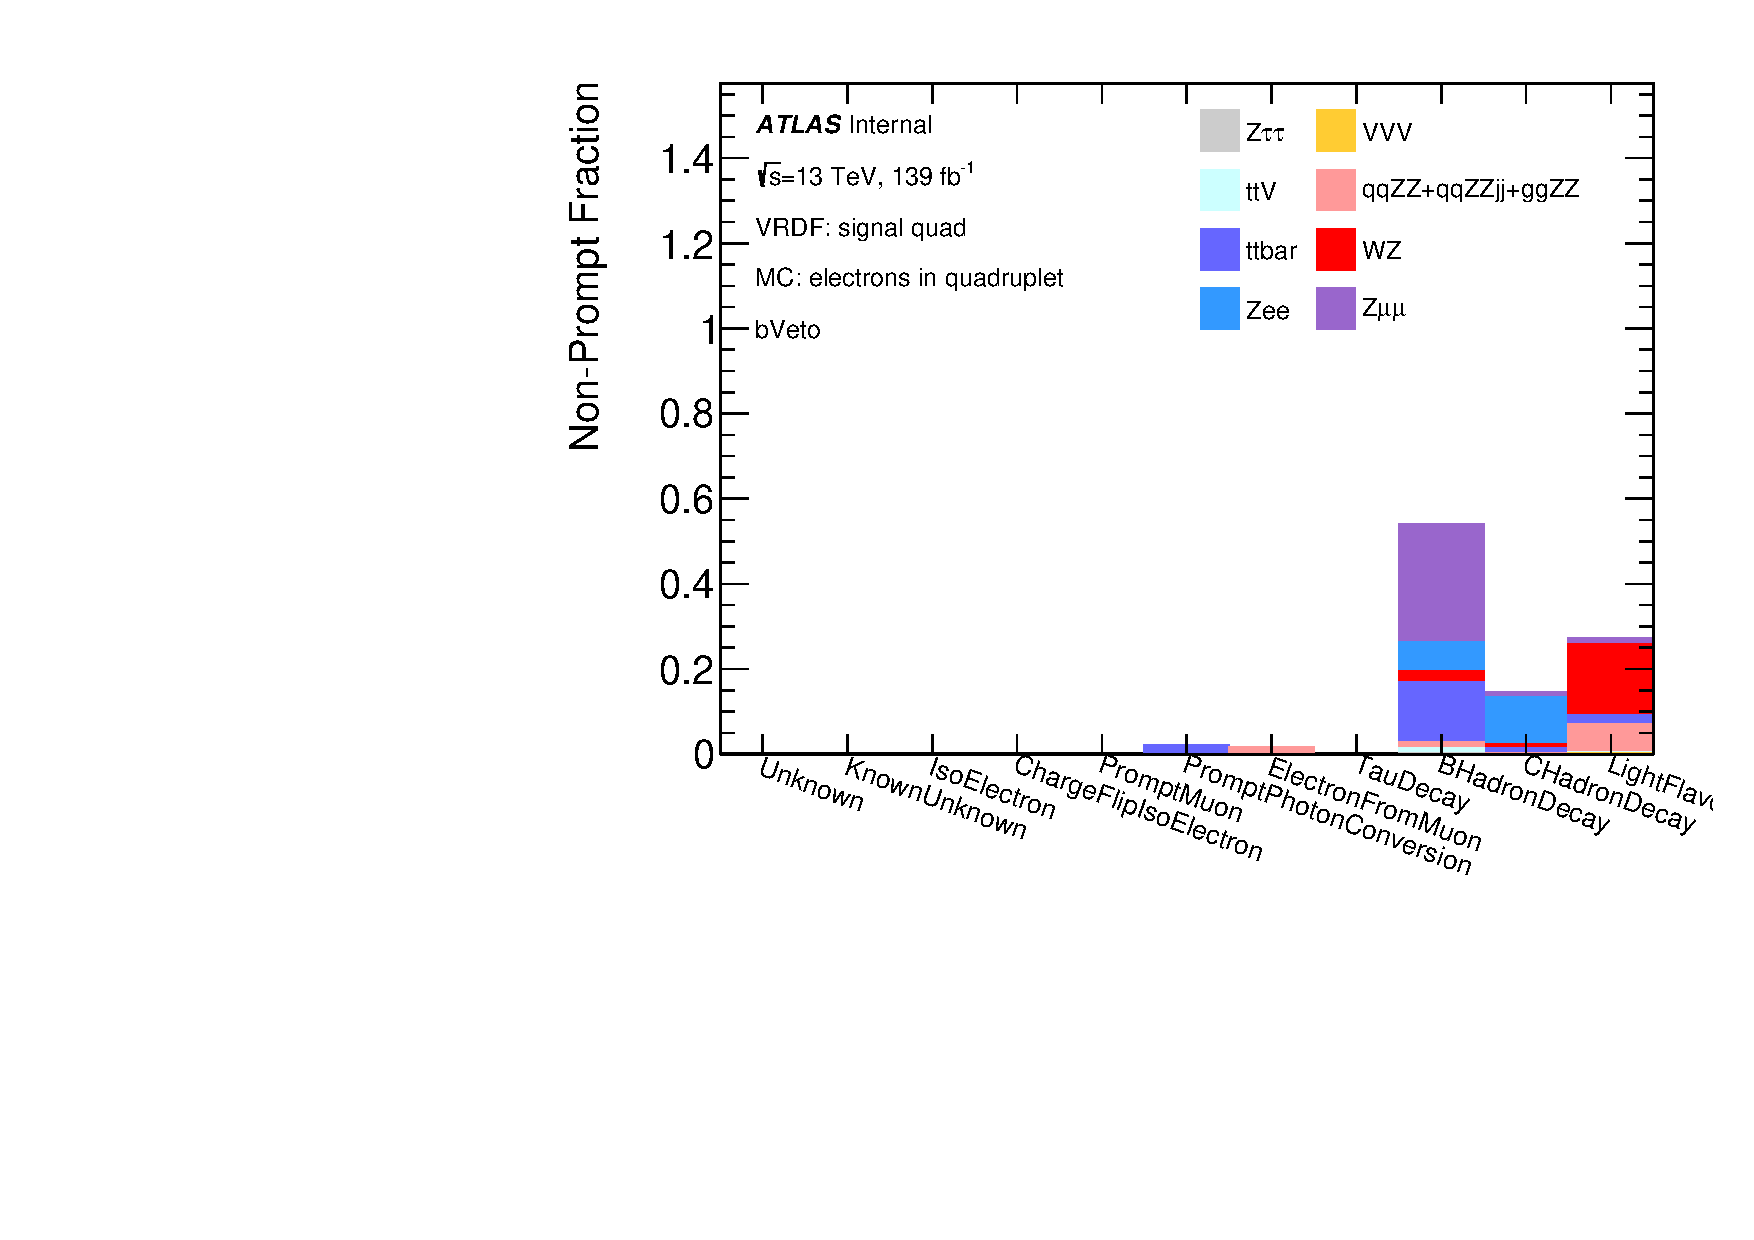
\includegraphics[width=.9\linewidth]{figures/Analysis/Background/NonPromptCRDFSignal_Electronss_bVeto.pdf}
        \caption{Non-prompt electrons in VRDF.\label{fig:VRDF_Elec_NonPromptComp}}
    \end{subfigure}
    \begin{subfigure}{.48\textwidth}
        \centering
        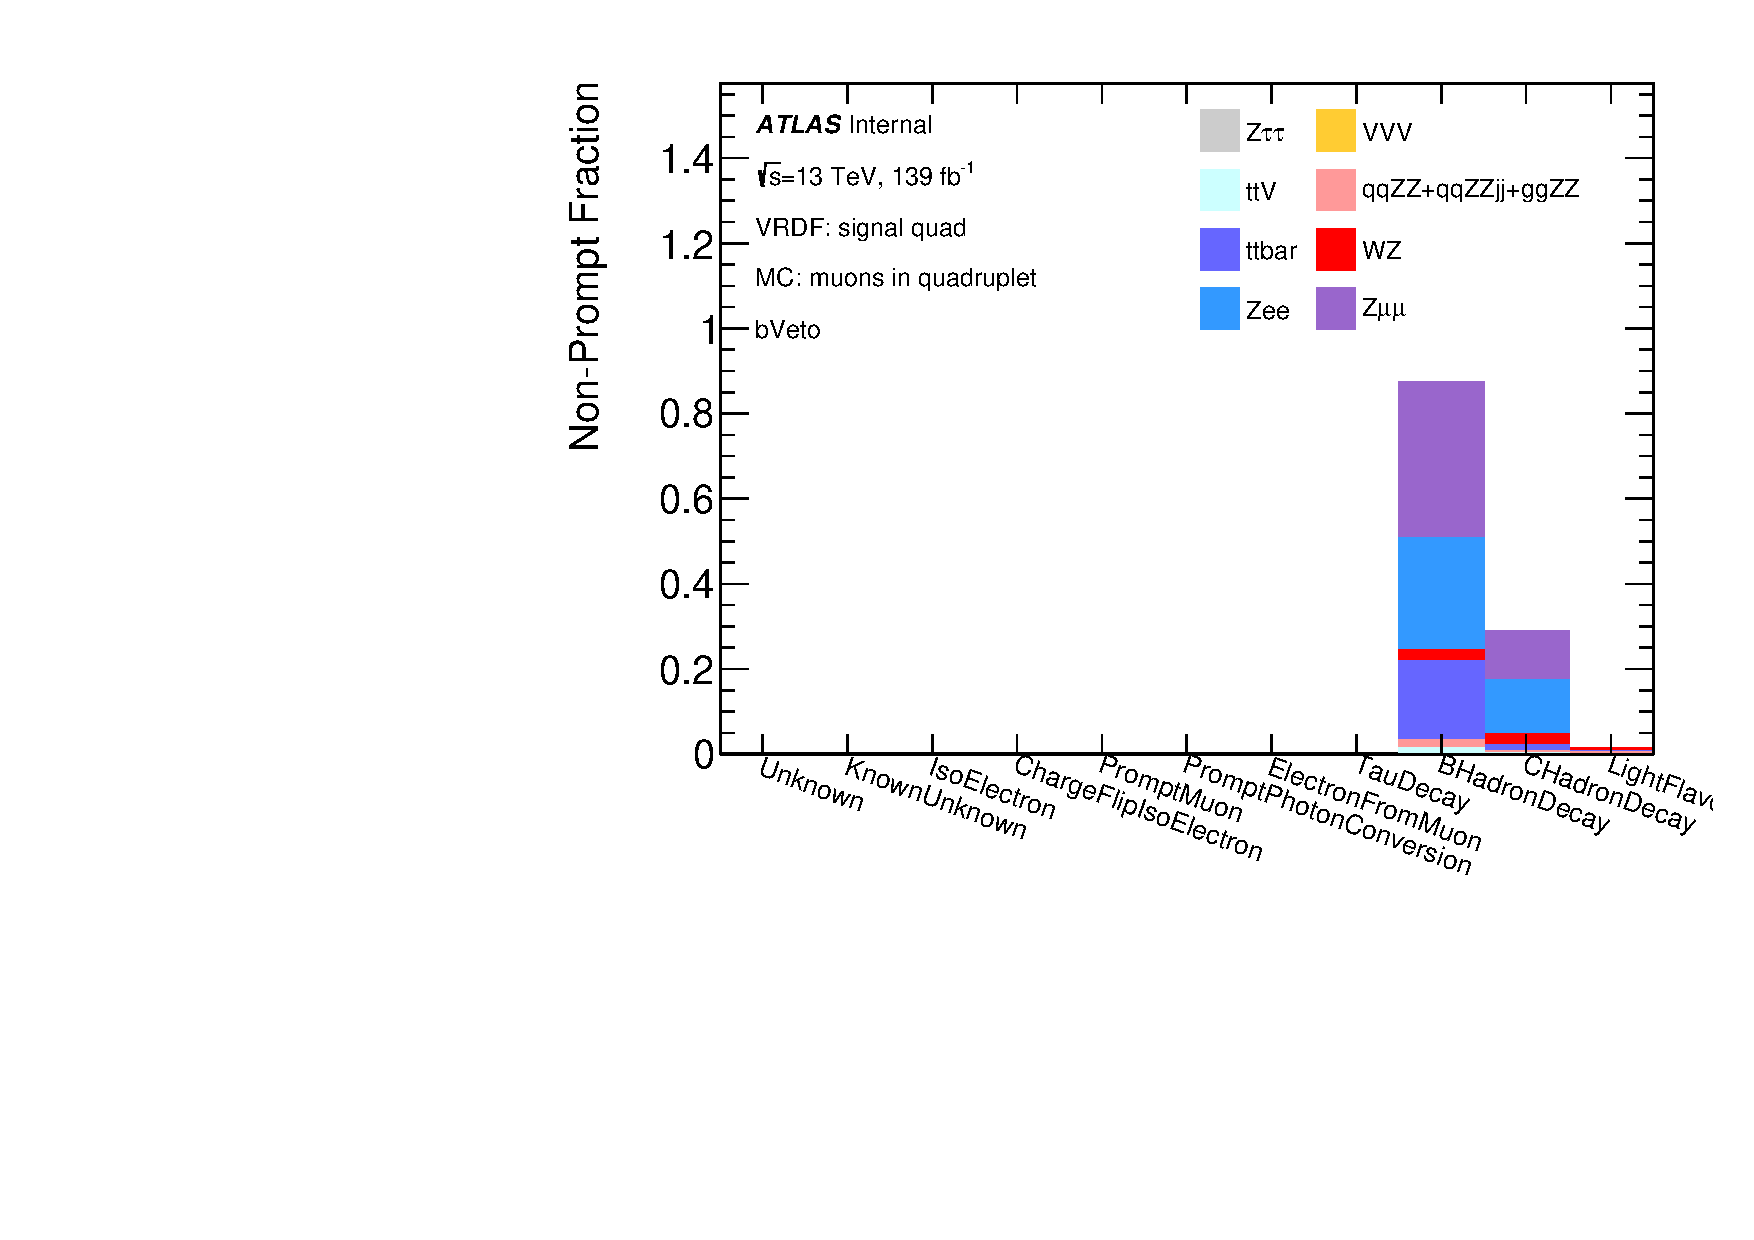
\includegraphics[width=.9\linewidth]{figures/Analysis/Background/NonPromptCRDFSignal_Muons_bVeto.pdf}\\
        \caption{Non-prompt muons in VRDF.\label{fig:VRDF_Muon_NonPromptComp}}
    \end{subfigure}
    \begin{subfigure}{.48\textwidth}
        \centering
        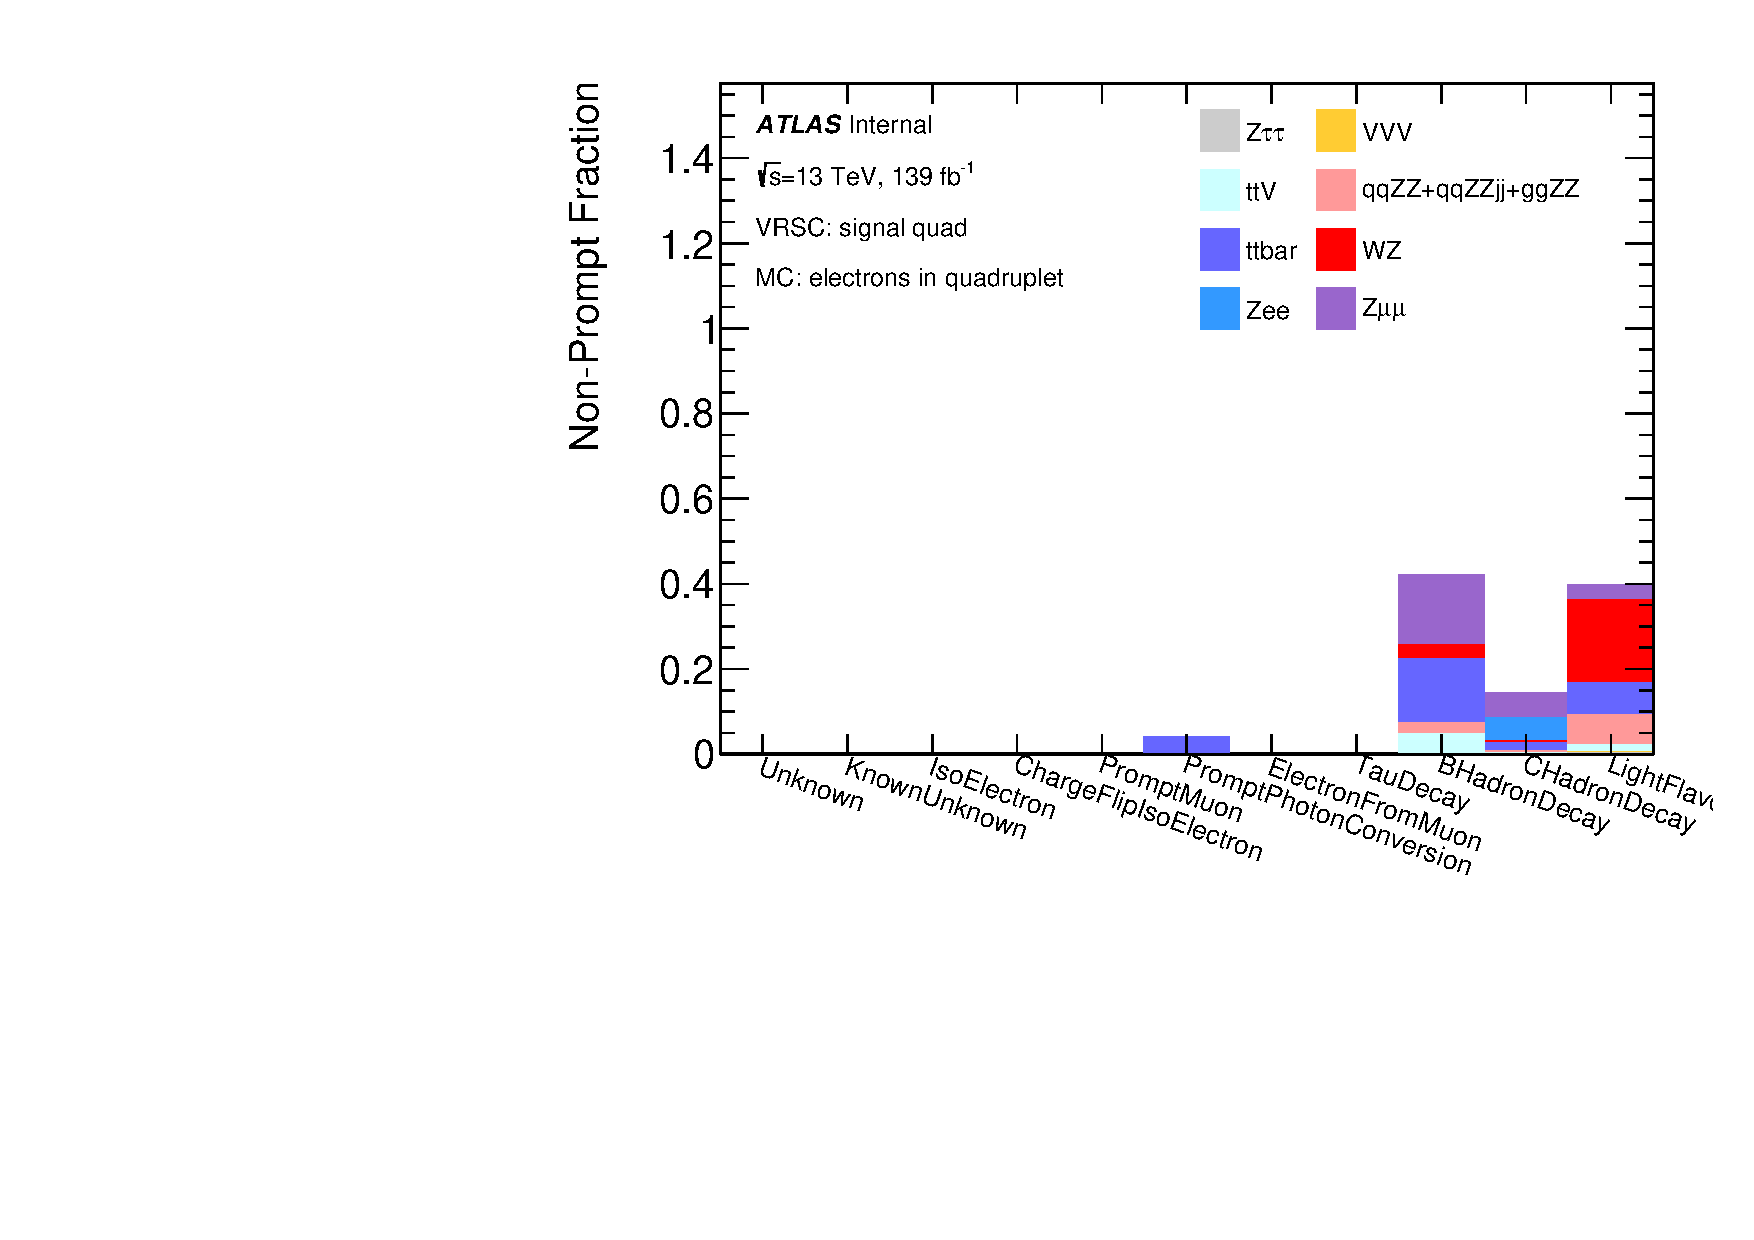
\includegraphics[width=.9\linewidth]{figures/Analysis/Background/NonPromptCRSCSignal_Electrons_.pdf}
    \caption{Non-prompt electrons in VRSC.\label{fig:VRSC_Elec_NonPromptComp}}
    \end{subfigure}
    \begin{subfigure}{.48\textwidth}
        \centering
        {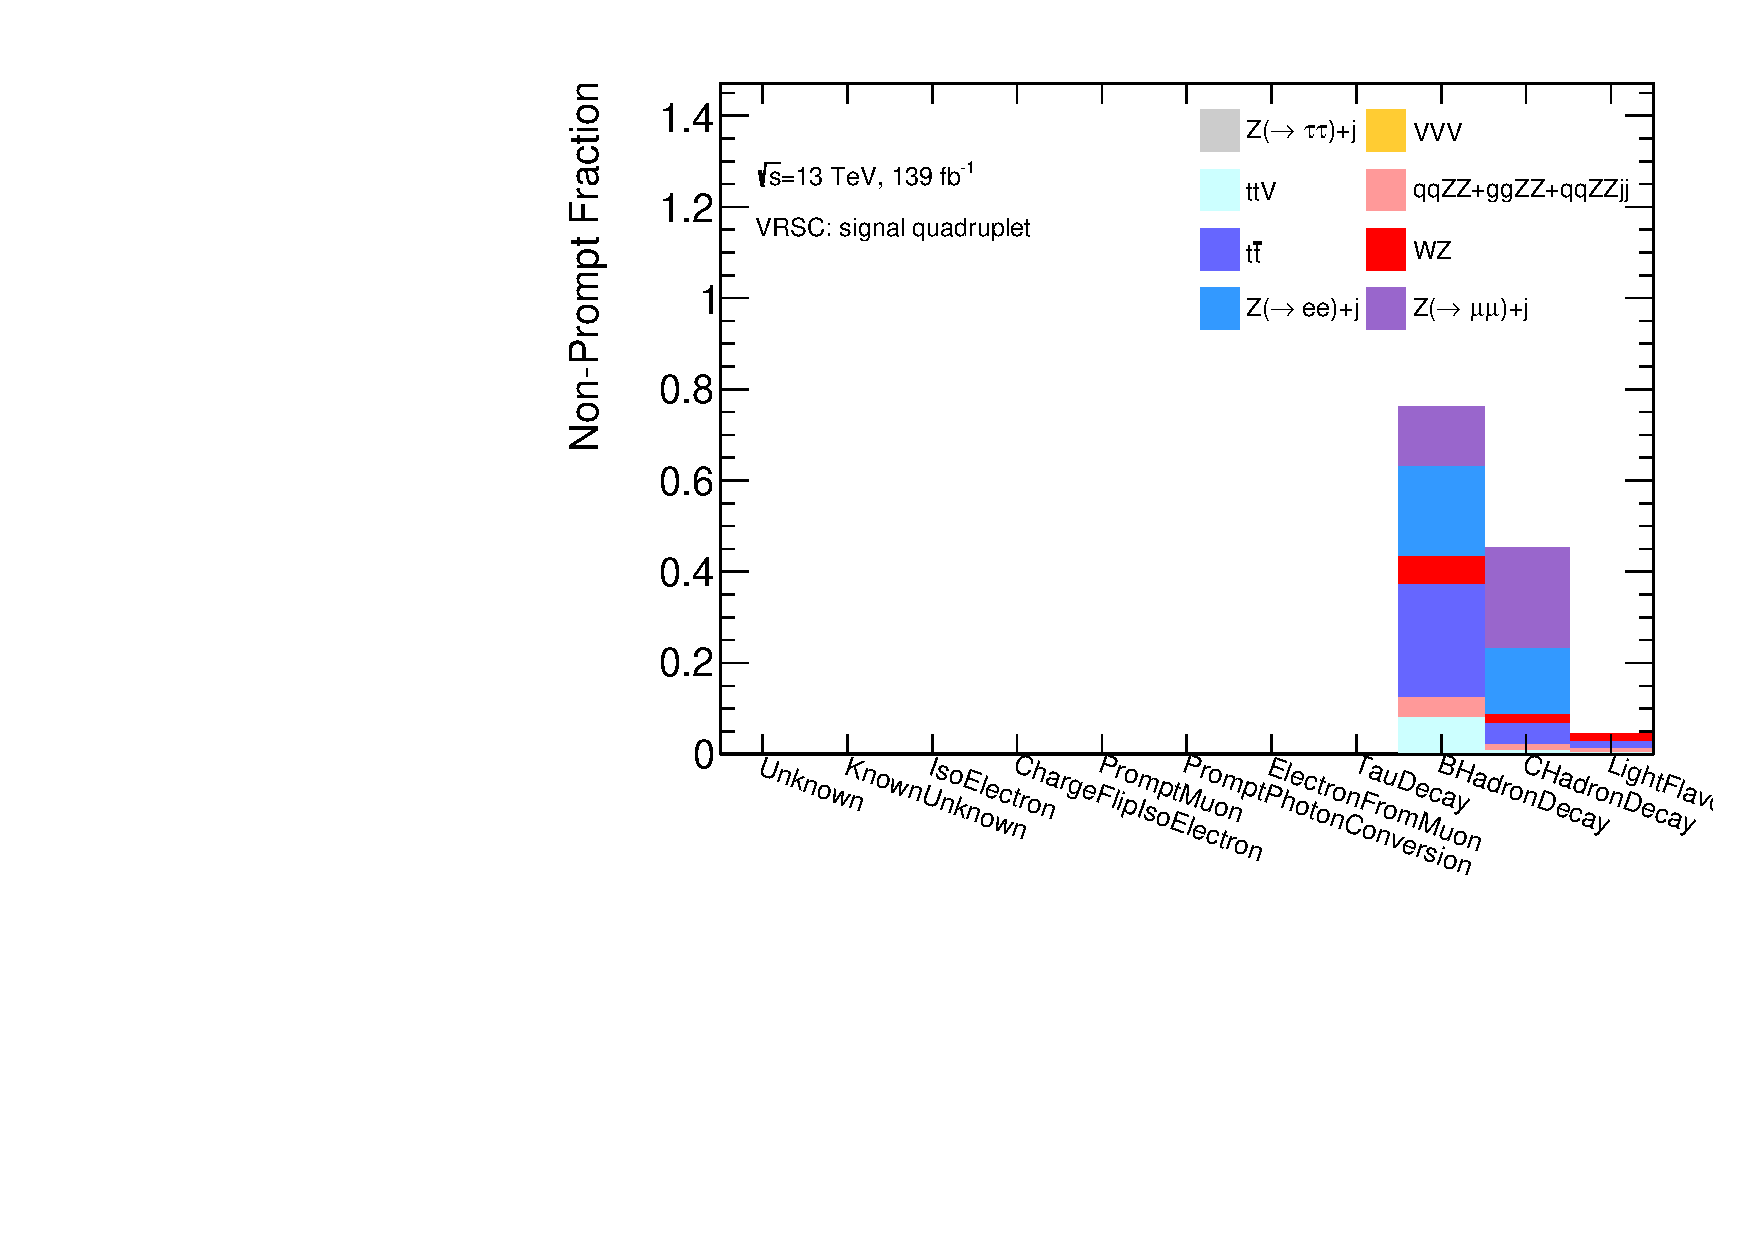
\includegraphics[width=.9\linewidth]{figures/Analysis/Background/NonPromptCRSCSignal_Muons_.pdf}}\\
        \caption{Non-prompt muons in VRSC.\label{fig:VRSC_Muon_NonPromptComp}}
    \end{subfigure}
    \caption{ Sources of non-prompt electrons and muons in the different flavors and the same charge validation regions. \label{fig:VRNonPromptComposition}}
\end{figure}

The fake backgrounds for the validation regions are estimated by applying the fake factor to each baseline-anti-signal leptons in the not-signal quadruplet, as discussed in Section \ref{subsubsec:EstimationStrategy}. Figure \ref{subfig:VRDFMCRed} shows the data and the predicted MC yield in VRDF as a function of $m_{4\ell}$ where the fake backgrounds are estimated from $Z+jets$, $t\bar{t}$, and $WZ$ MC predictions. Figure \ref{subfig:VRDFFF} shows the same, but the non-prompt background events are estimated using the fake factor method. Similarly, figures \ref{subfig:VRSCMCRed} and \ref{subfig:VRSCFF} show the yields as a function of $m_{4\ell}$ in the same charge validation region. Both regions have similar characteristics, and the fake background dominates the event yield with some contribution from other physics processes.

The systematic gray bands in figures \ref{subfig:VRDFFF} and \ref{subfig:VRSCFF} include the total systematic and statistical uncertainties from the fake factor method, as well as the uncertainties on PDF, QCD scale, and strong coupling ($\alpha_{S}$) on the $qqZZ,~qqZZjj~\&~ggZZ$ MC prediction. The bands also include the uncertainties in the cross-section measurements of the $ttZ$ and $VVV$ processes. The treatment of the systematic theoretical uncertainties is the same as that of the signal region, which will be discussed in Section \ref{subsec:TheoryUnc}. Other experimental uncertainties related to the lepton reconstruction and identification, trigger, and luminosity discussed in Section \ref{subsec:ExpUnc} are assumed to be negligible for the validation regions. For most bins in both regions, the data and MC yield are compatible within the $1\sigma$ band of the total uncertainties. Additionally, the agreement between data and MC simulation is better when the reducible events are estimated using the fake factor method, thus, fully validating the method. Moreover, the estimate from the fake factor method is robust in estimation regions where the non-prompt lepton composition is different from that of the phase space where the fake factors were derived.

\begin{figure}[htb]
    \centering
    \begin{subfigure}{.48\textwidth}
        \centering
        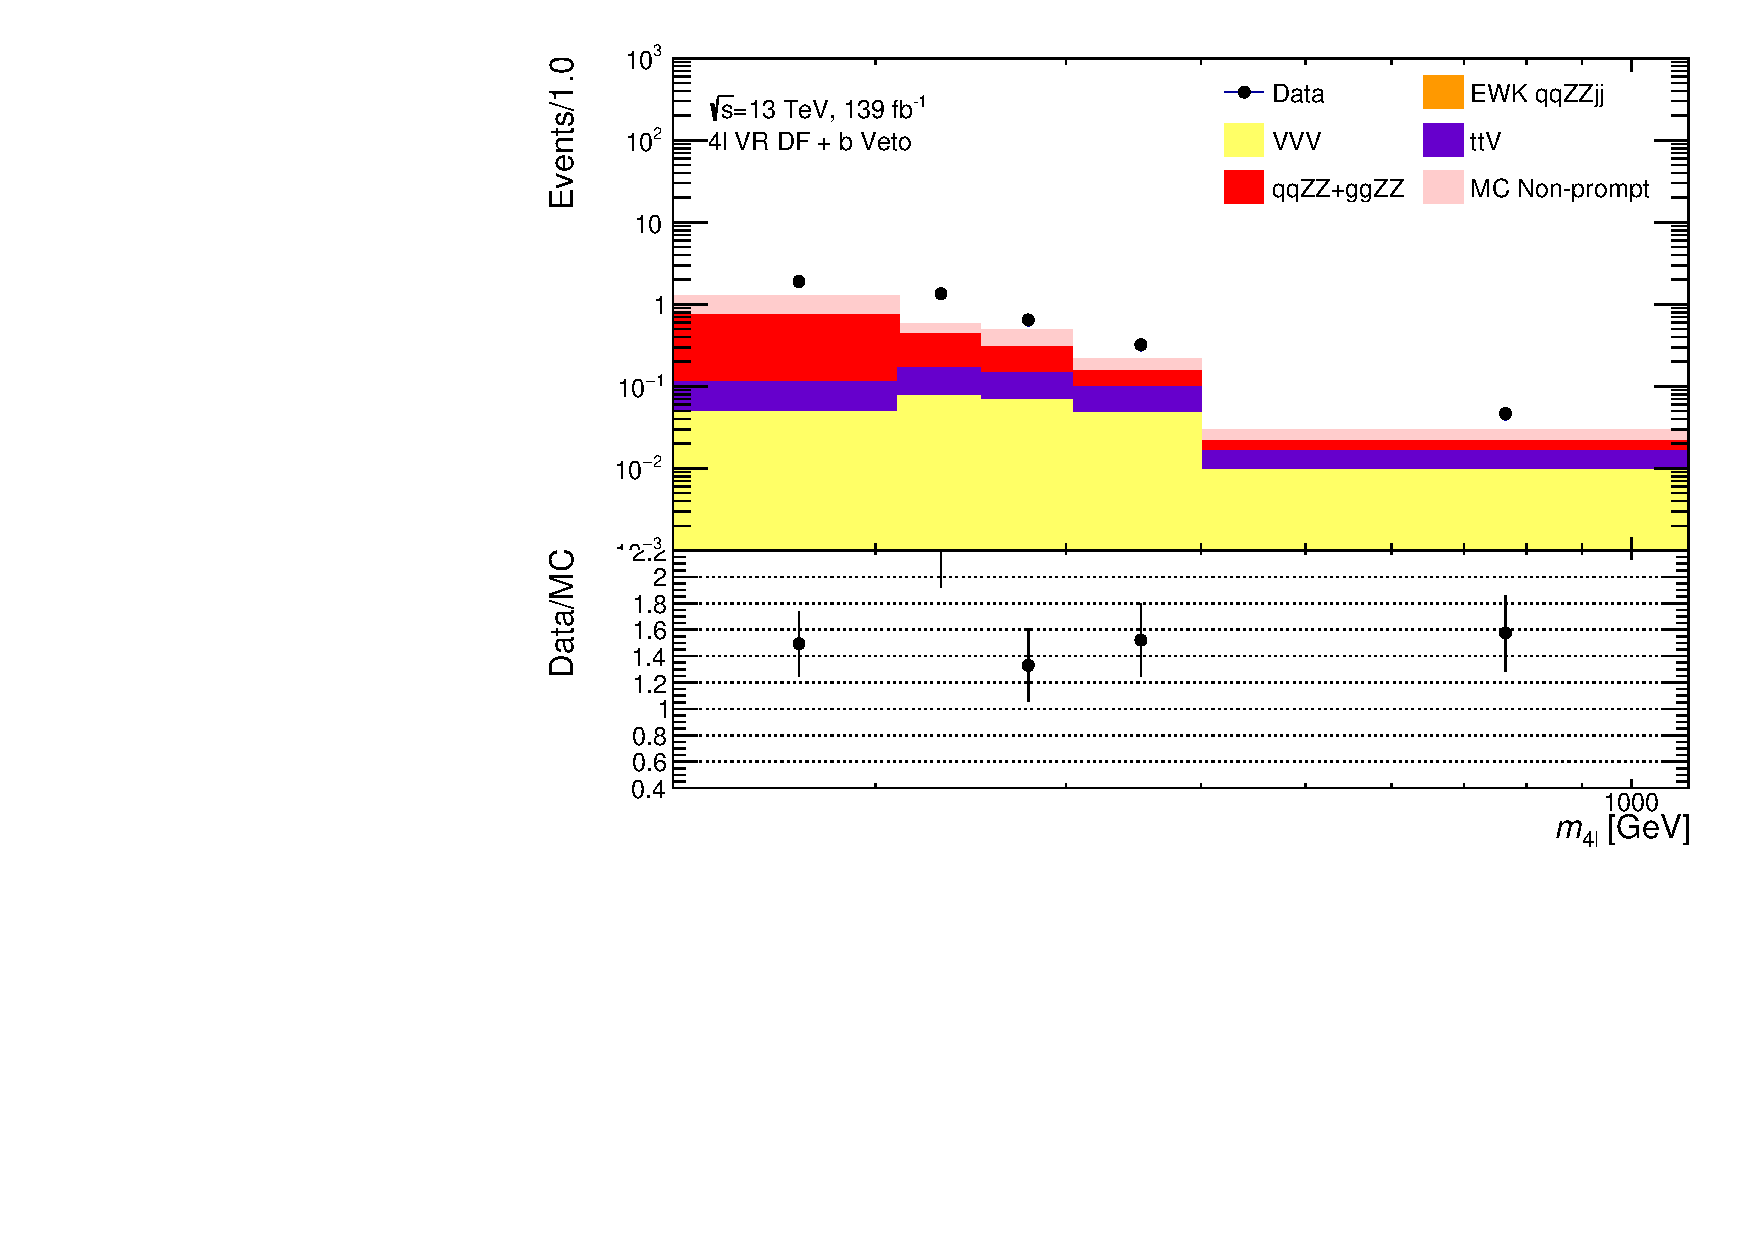
\includegraphics[width = 0.85\linewidth]{figures/Analysis/Background/Overlay_VRDF_RedMC_M4l.pdf}
        \caption{VRDF: MC predicted fake background.\label{subfig:VRDFMCRed}}
    \end{subfigure}
    \begin{subfigure}{.48\textwidth}
        \centering
        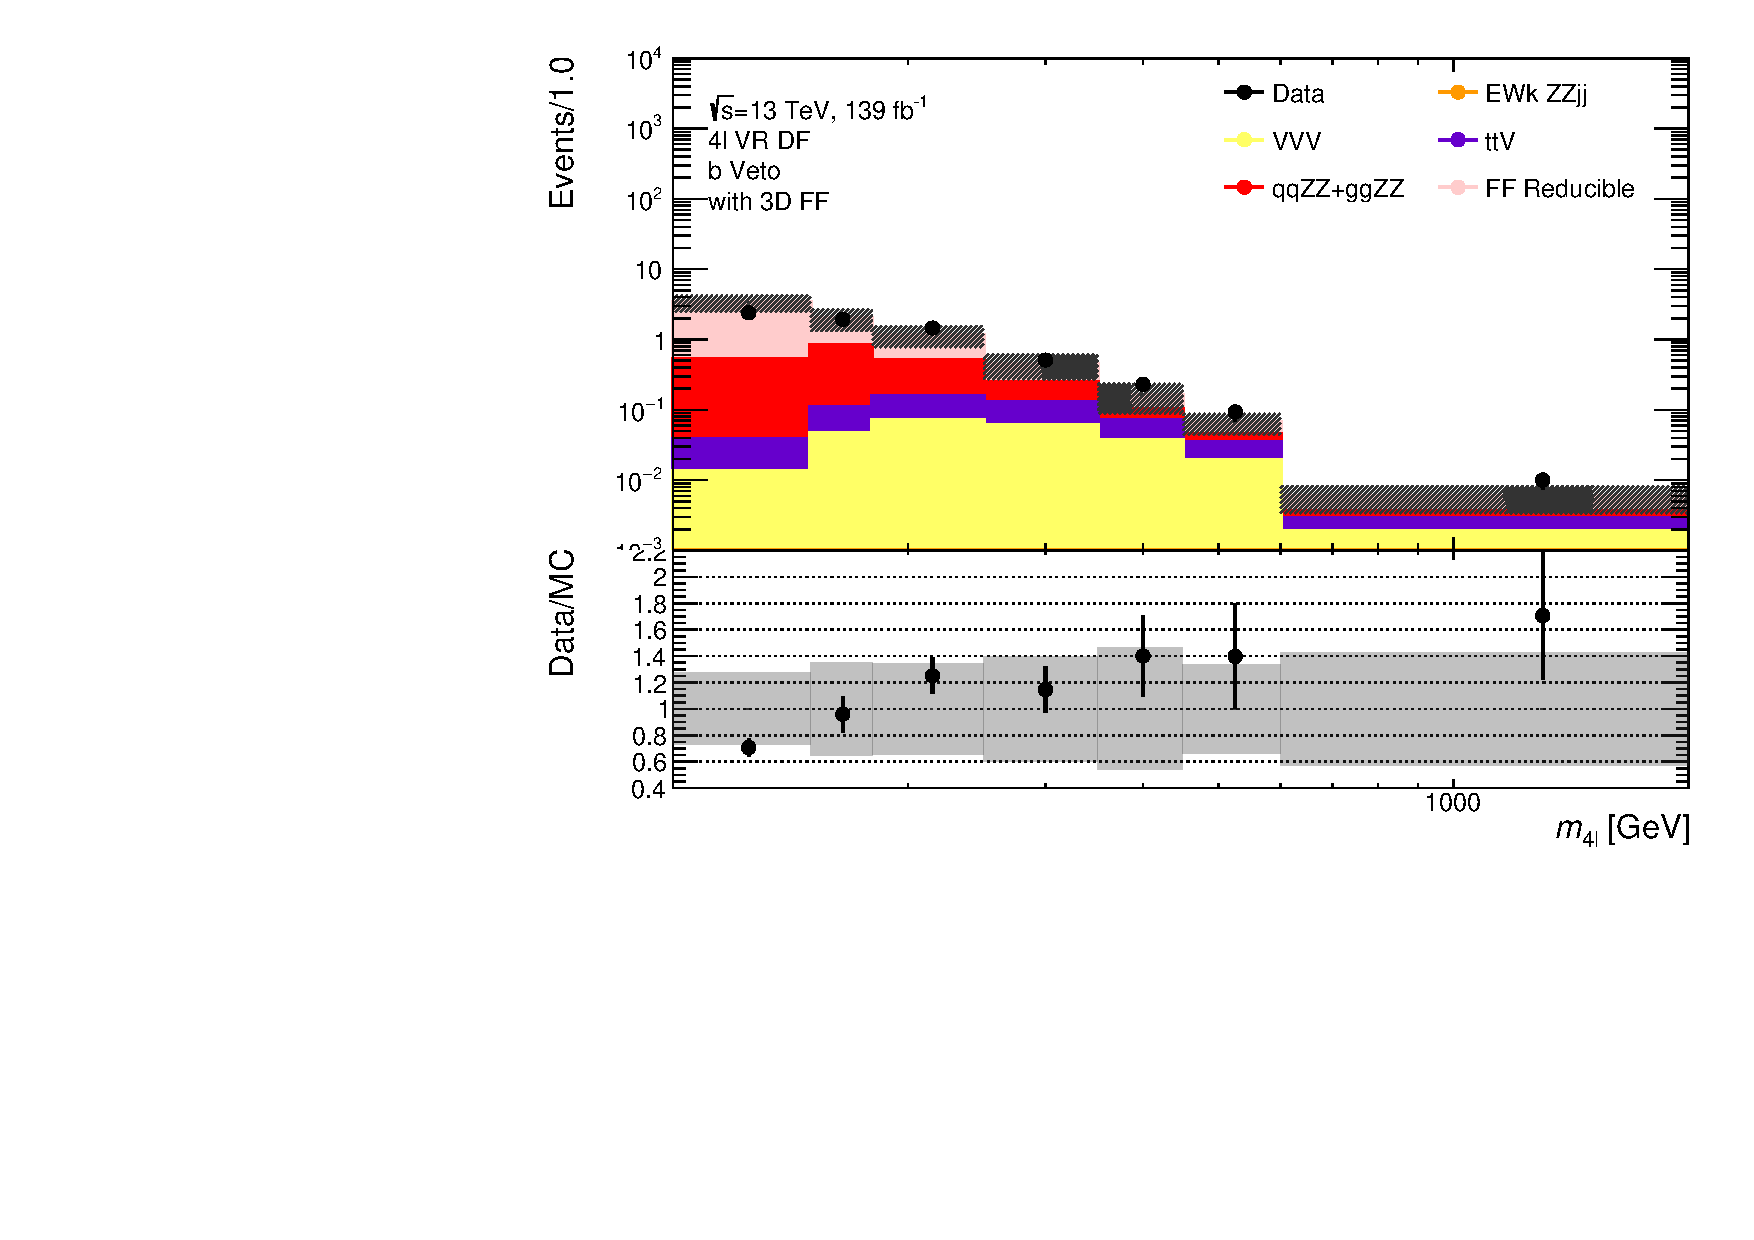
\includegraphics[width = 0.85\linewidth]{figures/Analysis/Background/Overlay_VRDF_FFApplied_M4l.pdf}\\
        \caption{ VRDF: FF estimate of fake background. \label{subfig:VRDFFF} }
    \end{subfigure}
    \begin{subfigure}{.48\textwidth}
        \centering
        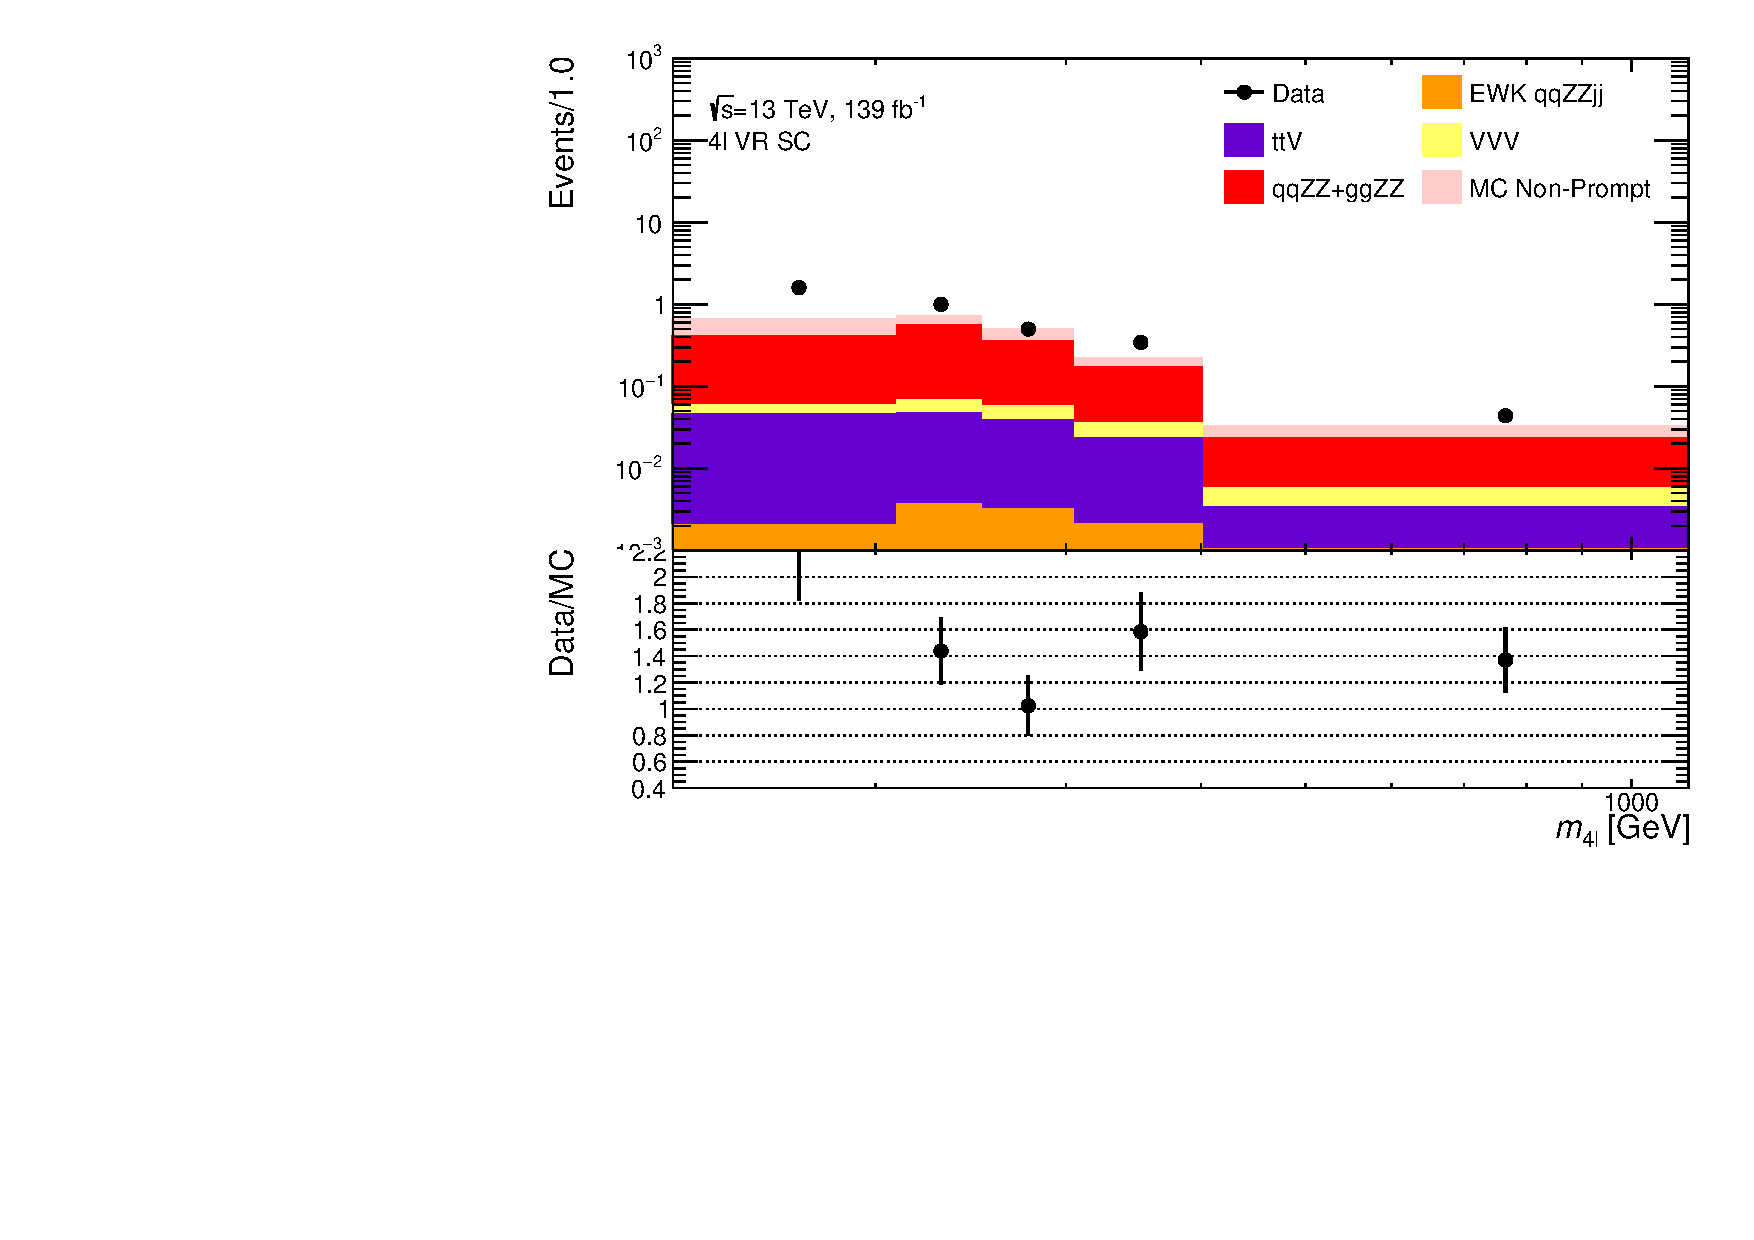
\includegraphics[width = 0.85\linewidth]{figures/Analysis/Background/Overlay_VRSC_RedMC_M4l.pdf}
        \caption{VRSC: MC predicted fake background.\label{subfig:VRSCMCRed}}
    \end{subfigure}
    \begin{subfigure}{.48\textwidth}
        \centering
        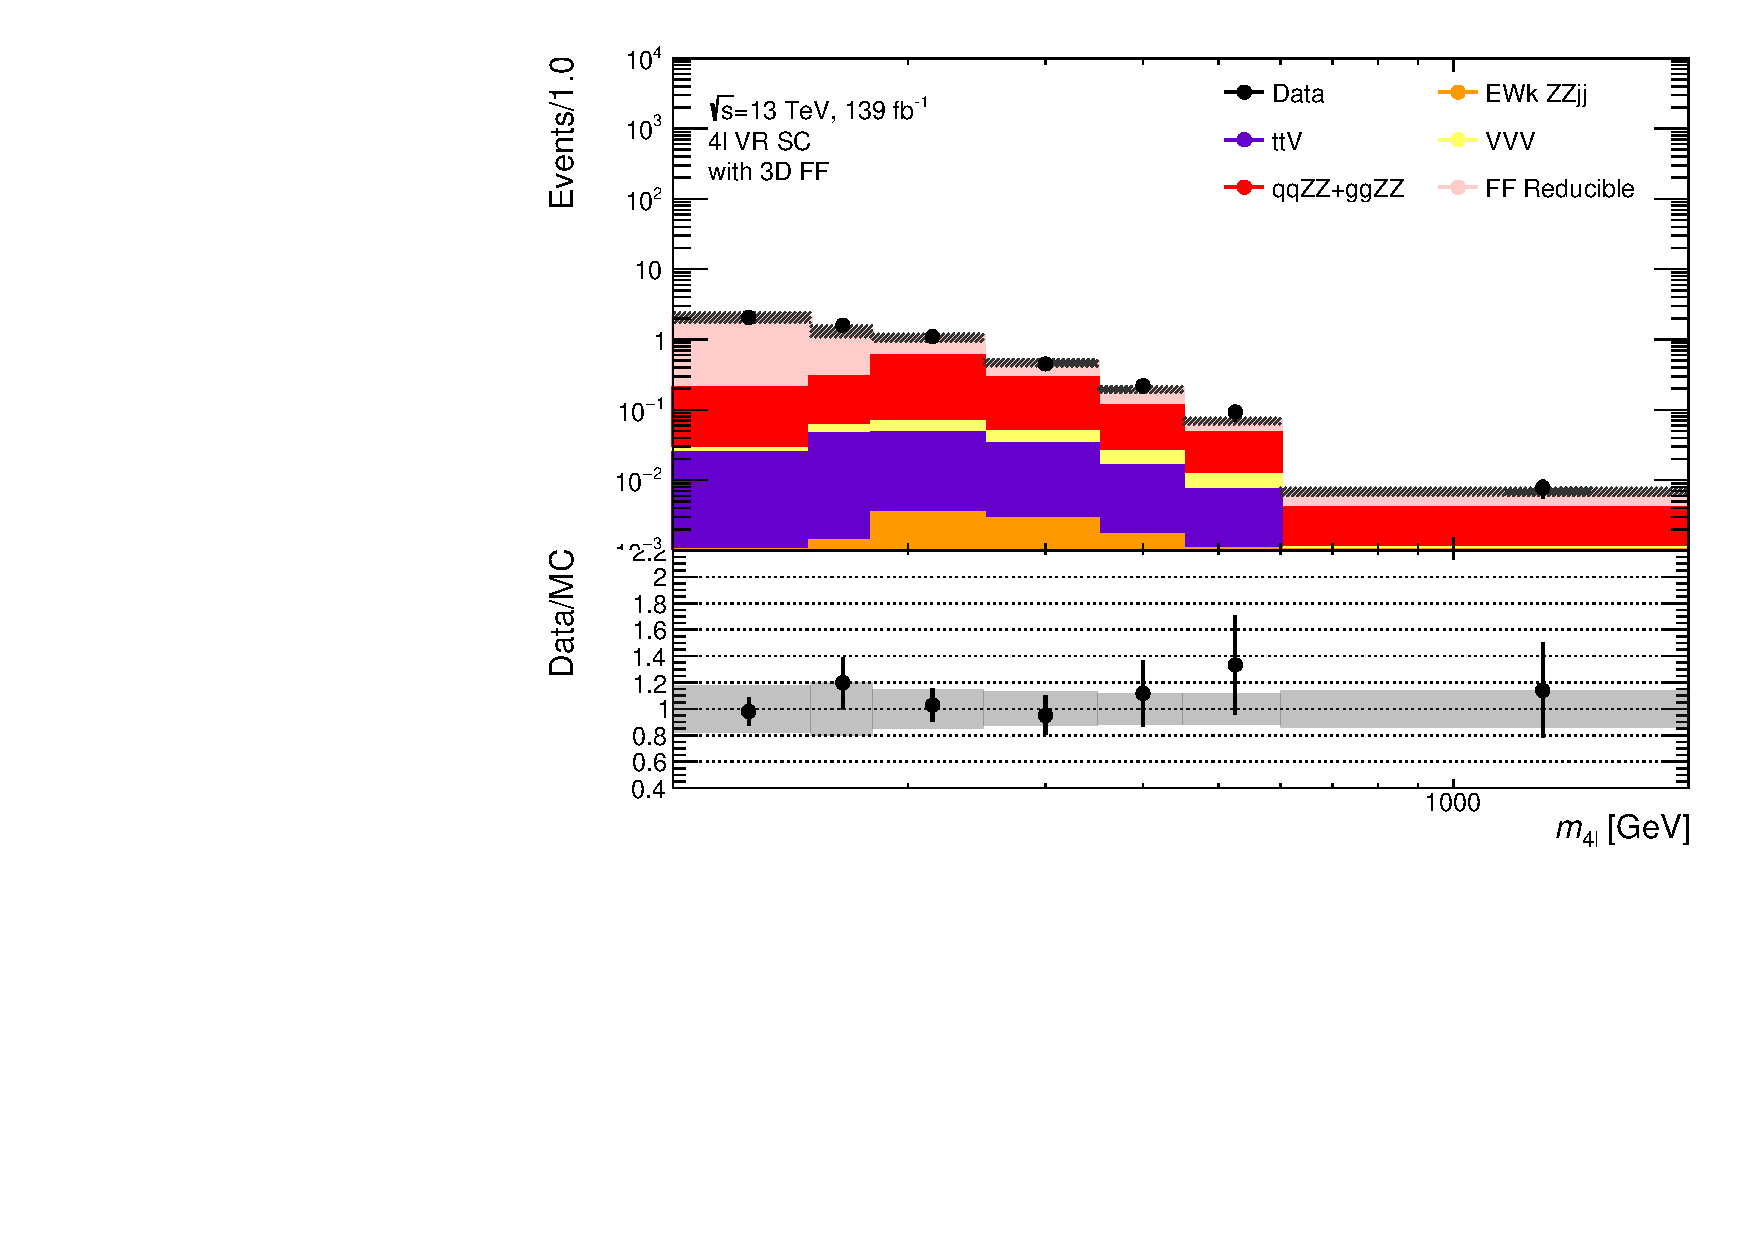
\includegraphics[width = 0.85\linewidth]{figures/Analysis/Background/Overlay_VRSC_FFApplied_M4l.pdf}
        \caption{VRSC: FF estimate of fake background.\label{subfig:VRSCFF}}
    \end{subfigure}
    \caption{ Comparison of data to the total MC prediction and fake background in the different flavor (top) and same charge (bottom) validation regions as a function of $\mFourL$.\label{fig:VRDataMCYield}}
\end{figure}

The data and MC yield comparisons for three kinematic observables, $p_{T}$ of leading lepton, $\eta$ of leading lepton, and the number of jets $n_{jets}$ are shown by Figures \ref{fig:AllDataMCYield_VRDF_pt1}, \ref{fig:AllDataMCYield_VRDF_eta1} and \ref{fig:AllDataMCYield_VRDF_njet}, respectively in VRDF. Similarly, Figures \ref{fig:AllDataMCYield_VRSC_pt1}, \ref{fig:AllDataMCYield_VRSC_eta1} and \ref{fig:AllDataMCYield_VRSC_njet}, show the data and MC yield for $p_{T}$ of leading lepton, $\eta$ of leading lepton and number of jets $n_{jets}$, respectively in VRSC. The data and MC prediction are compatible in most bins within total uncertainties in each validation region.

\begin{figure}[htb]
    \centering
    \begin{subfigure}{.48\textwidth}
        \centering
        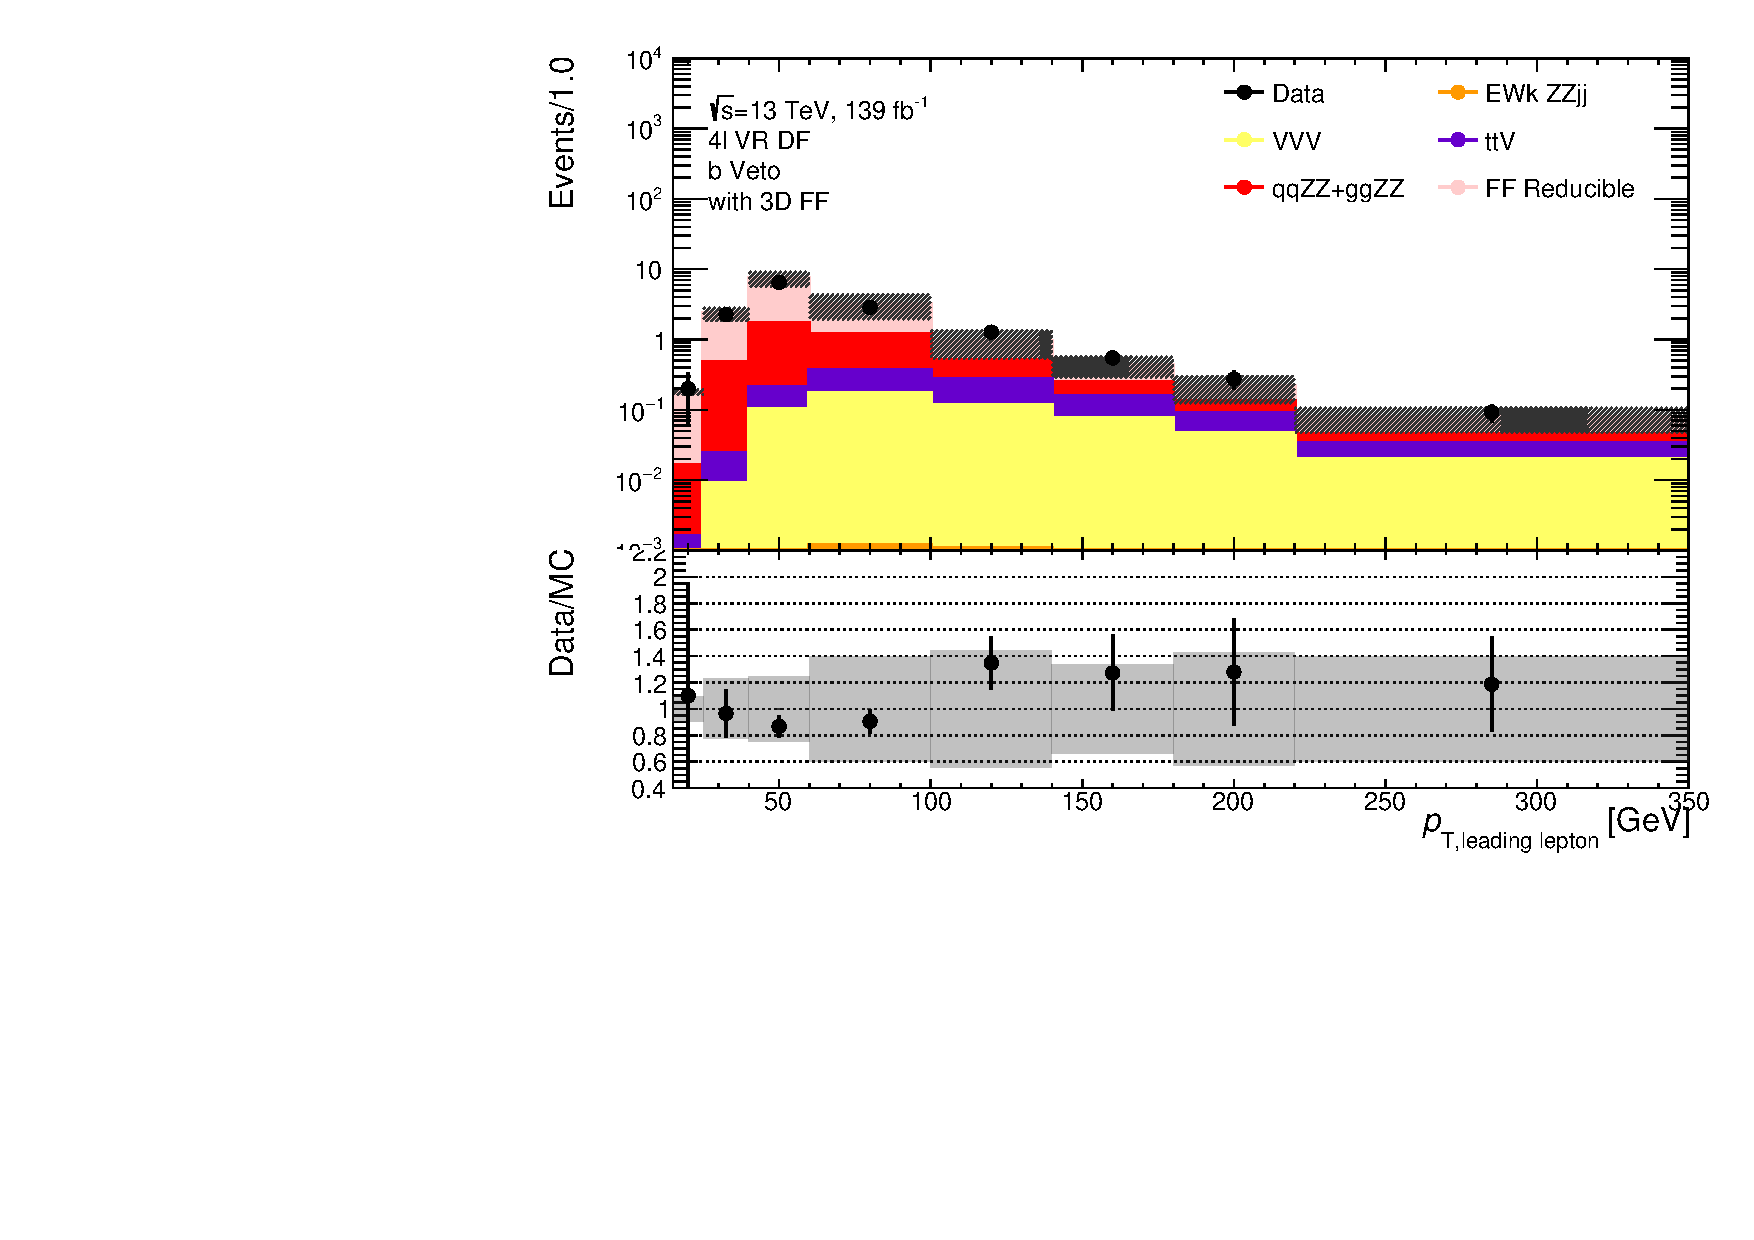
\includegraphics[width = 0.85\linewidth]{figures/Analysis/Background/Overlay_VRDF_FFApplied_pt1.pdf}
        \caption{VRDF: $p_{T,~leading~lepton}$ \label{fig:AllDataMCYield_VRDF_pt1} }
    \end{subfigure}
    \begin{subfigure}{.48\textwidth}
        \centering
        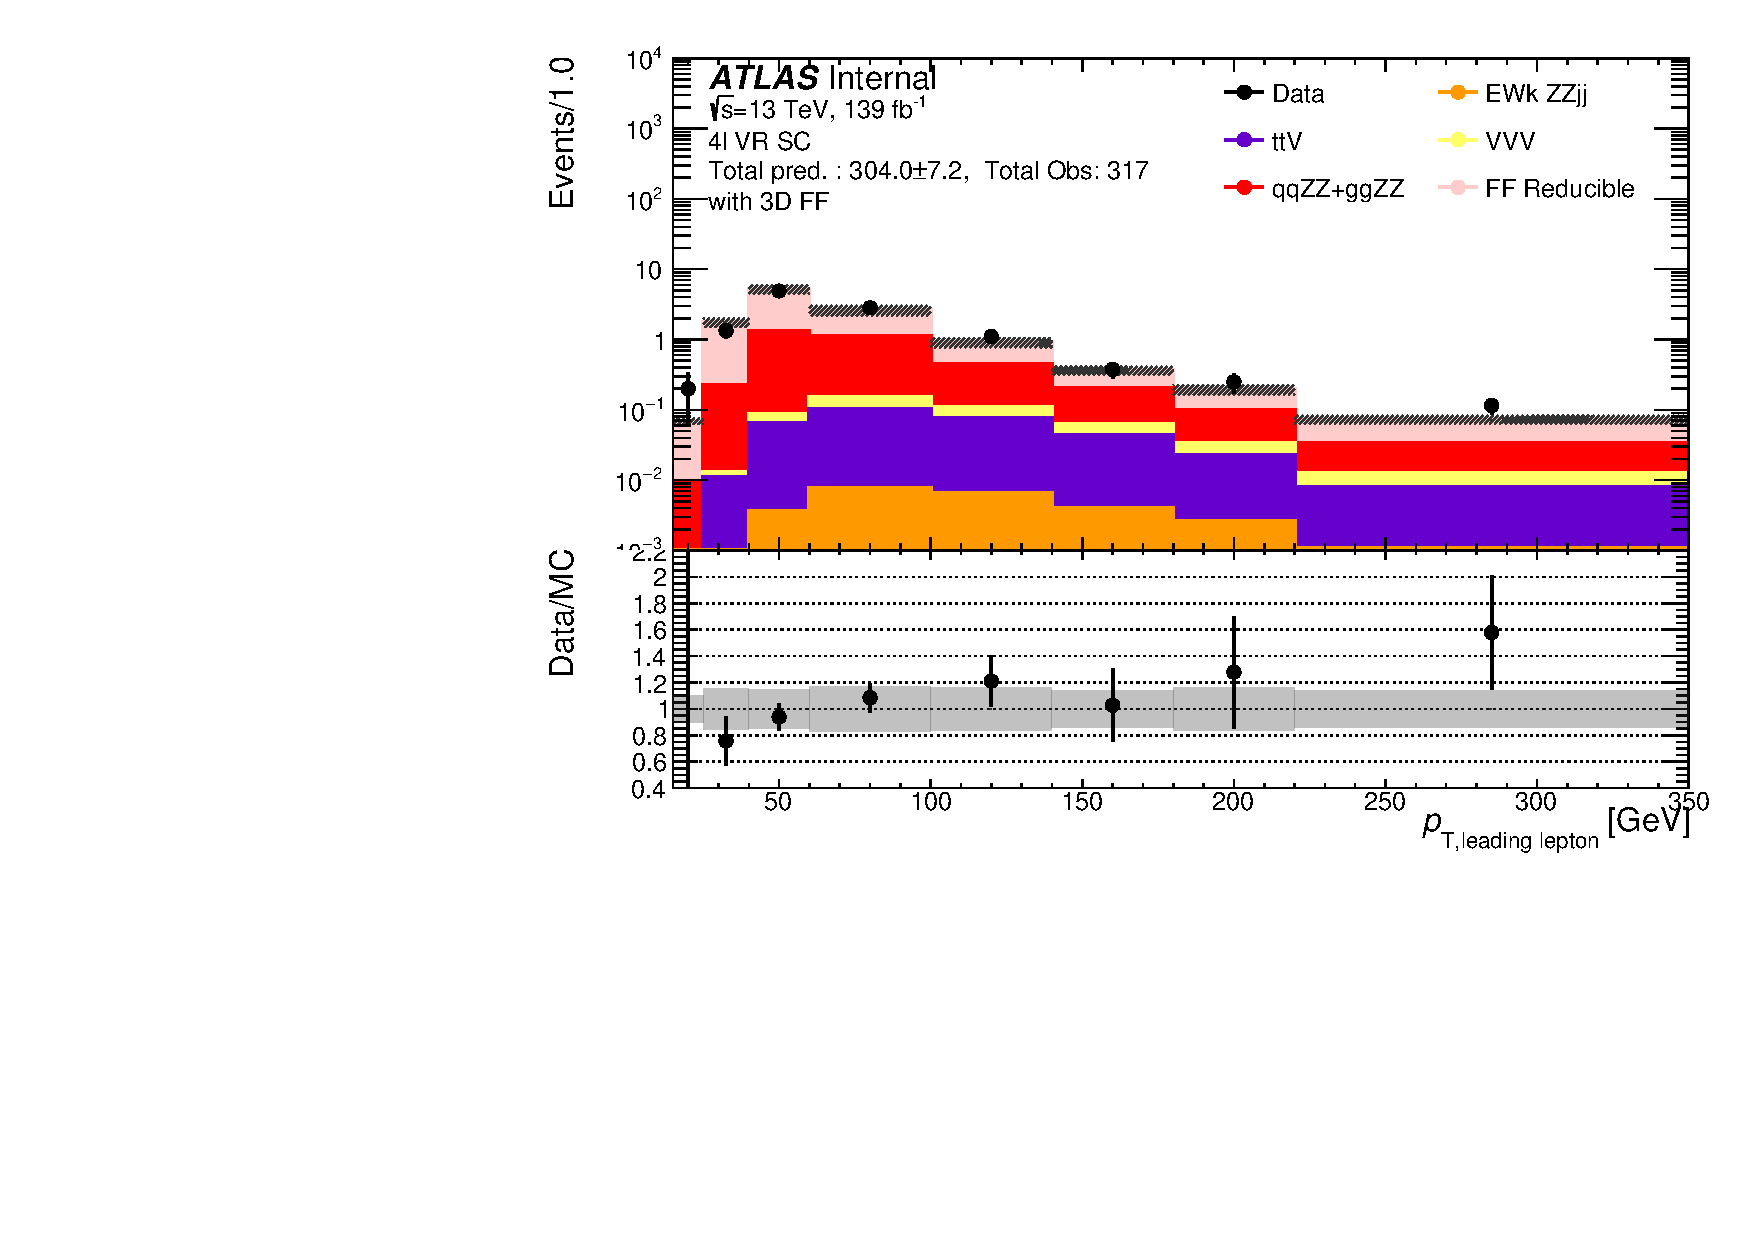
\includegraphics[width = 0.85\linewidth]{figures/Analysis/Background/Overlay_VRSC_FFApplied_pt1.pdf}
        \caption{VRSC: $p_{T,~leading~lepton}$ \label{fig:AllDataMCYield_VRSC_pt1} }
    \end{subfigure} \\
    \begin{subfigure}{.48\textwidth}
        \centering
        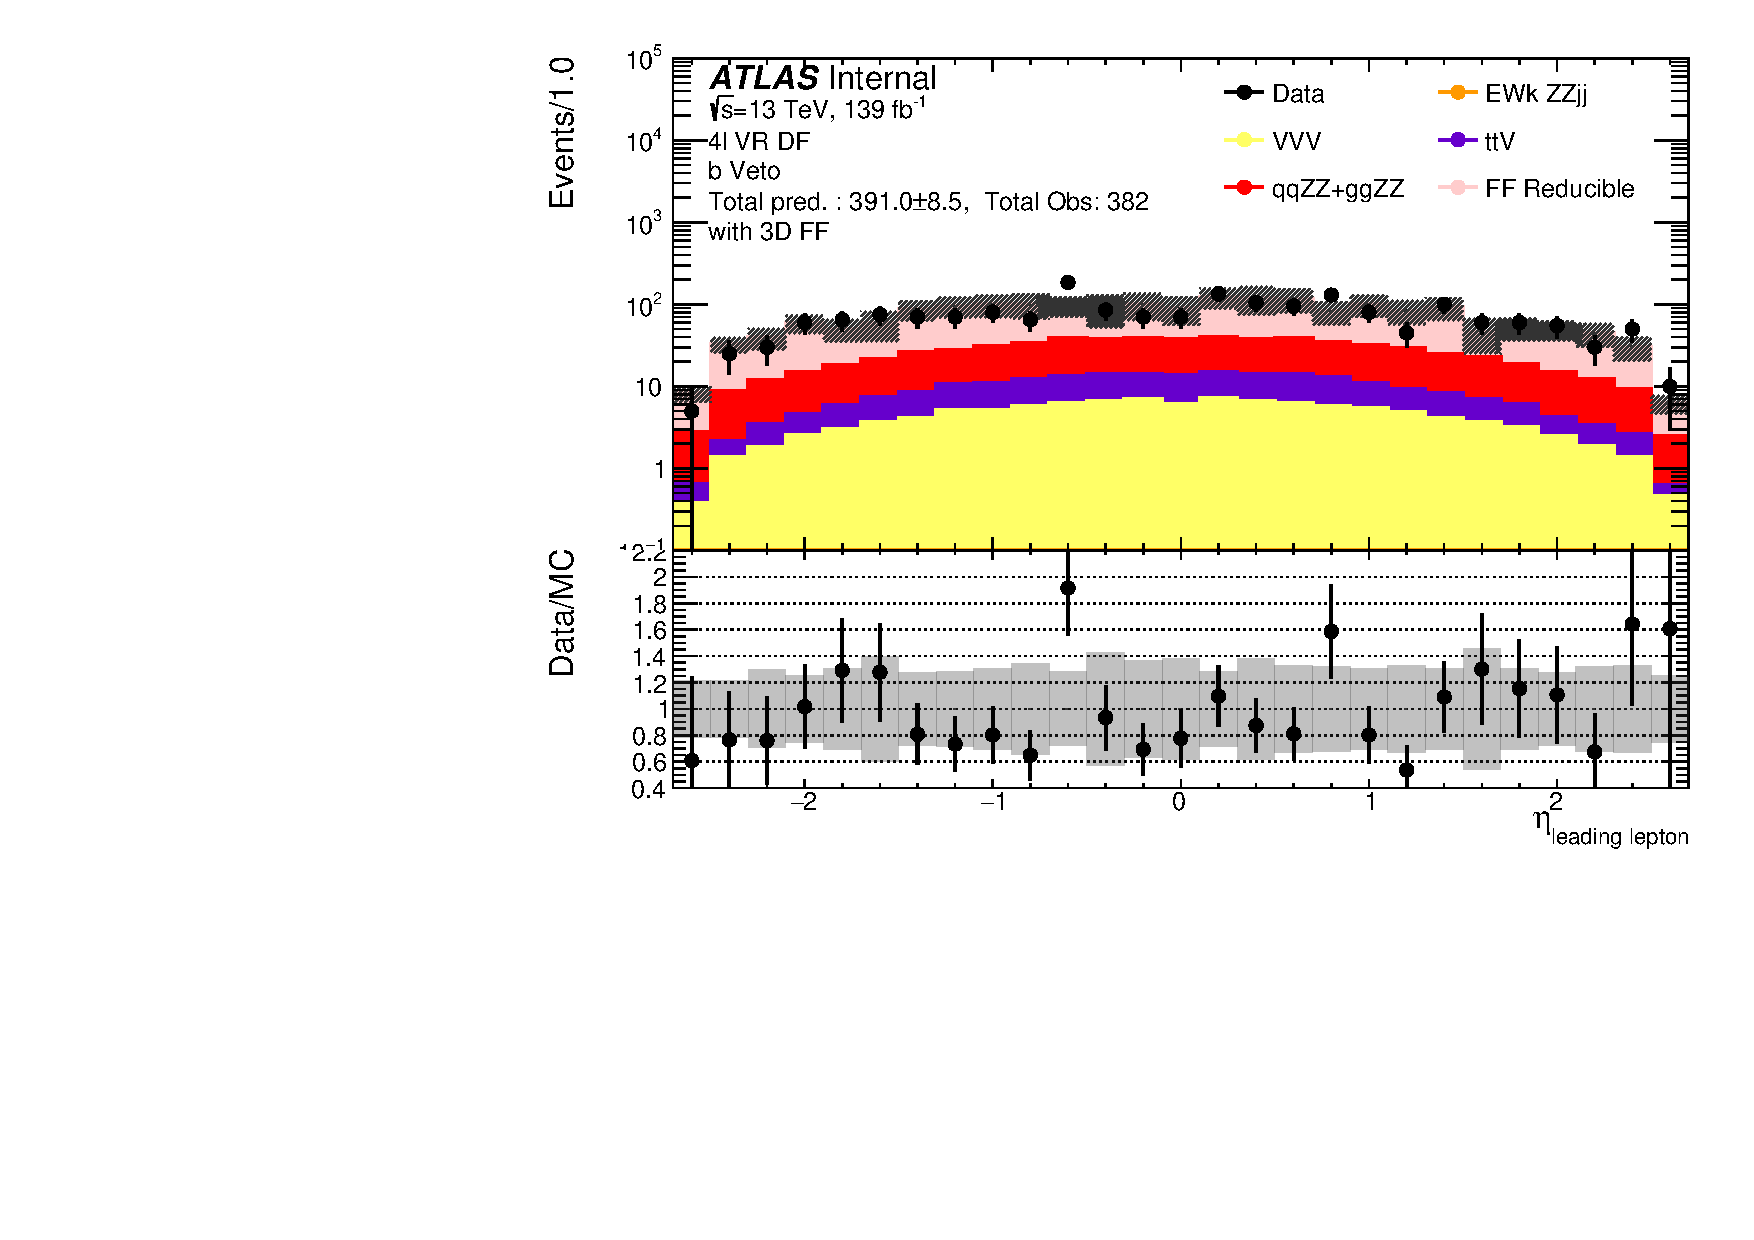
\includegraphics[width = 0.85\linewidth]{figures/Analysis/Background/Overlay_VRDF_FFApplied_eta1.pdf}
        \caption{VRDF: $\eta_{T,~leading~lepton}$ \label{fig:AllDataMCYield_VRDF_eta1} }
    \end{subfigure}
    \begin{subfigure}{.48\textwidth}
        \centering
        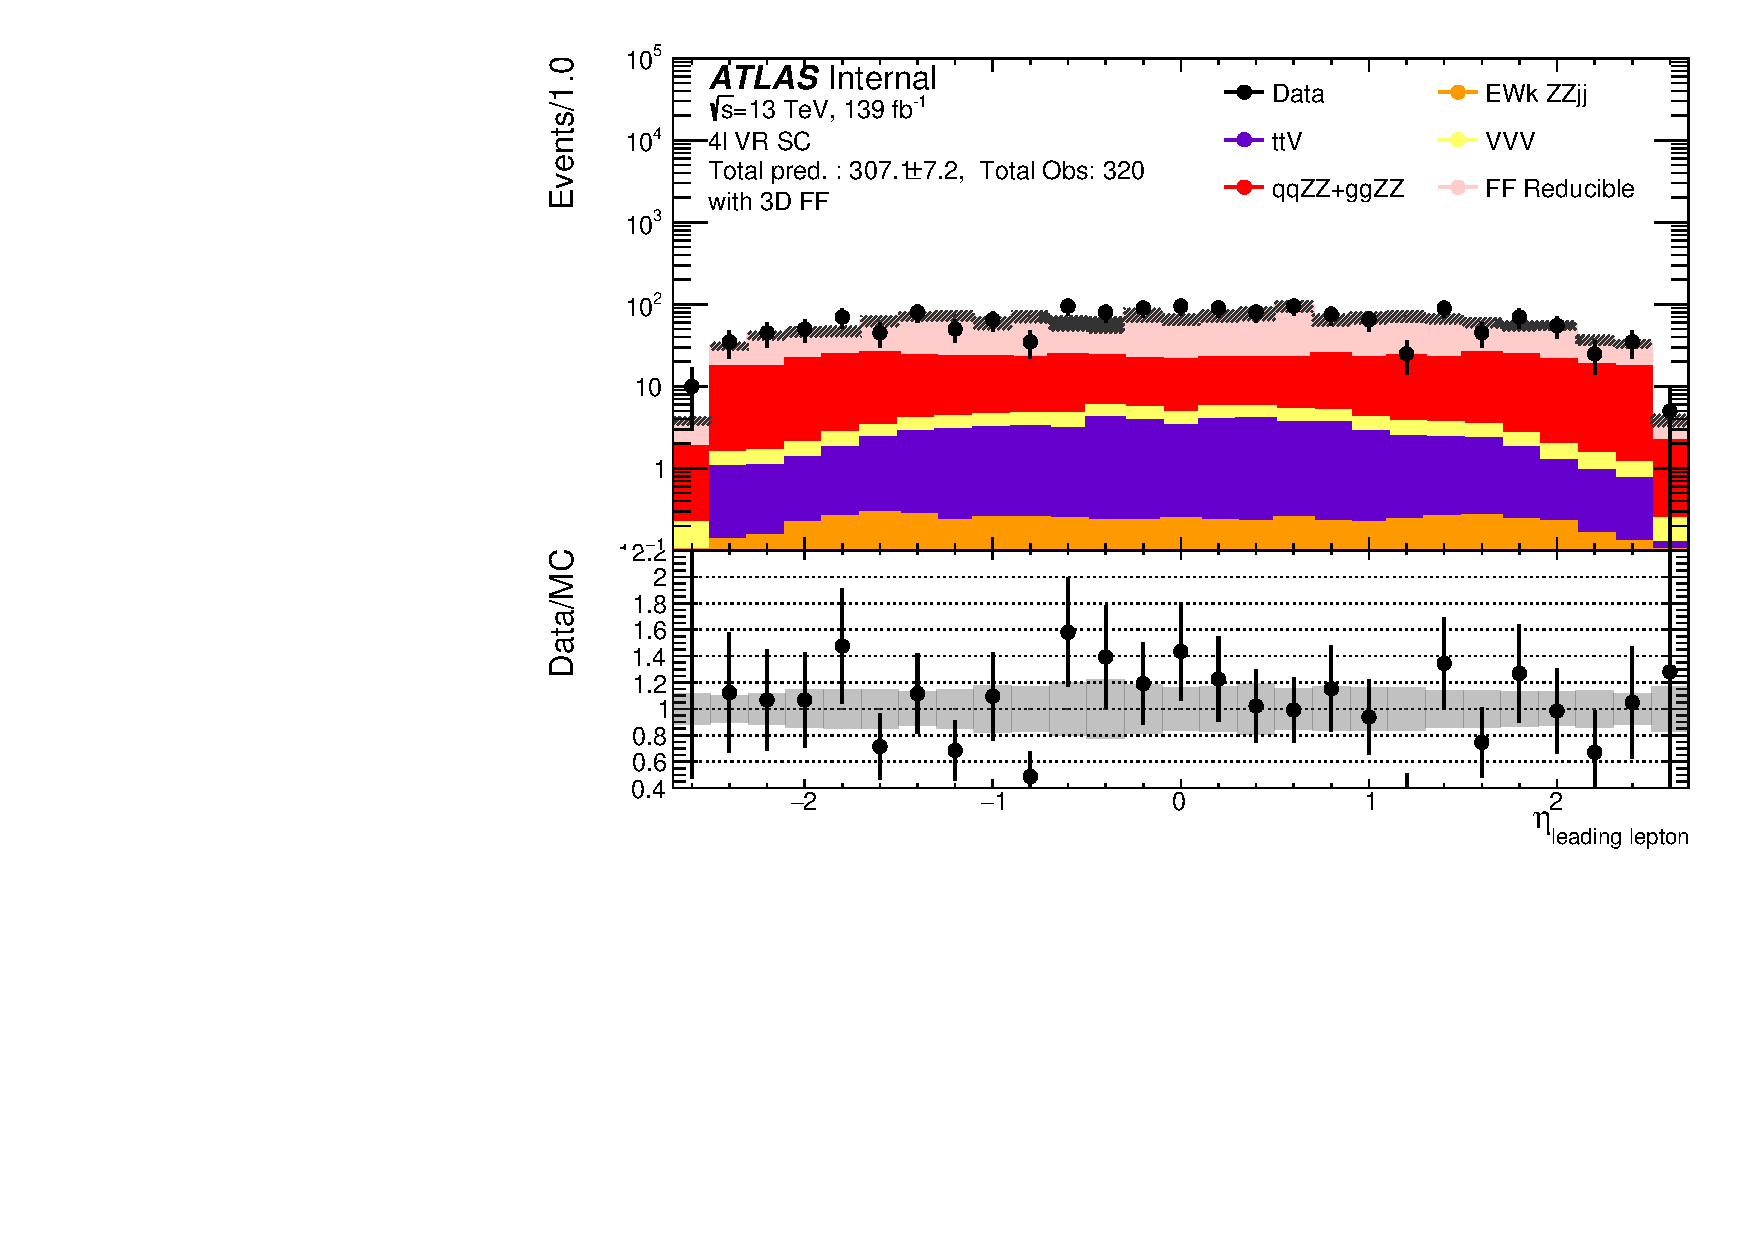
\includegraphics[width = 0.85\linewidth]{figures/Analysis/Background/Overlay_VRSC_FFApplied_eta1.pdf}
        \caption{VRSC: $\eta_{T,~leading~lepton}$ \label{fig:AllDataMCYield_VRSC_eta1} }
    \end{subfigure}\\
    \begin{subfigure}{.48\textwidth}
        \centering
        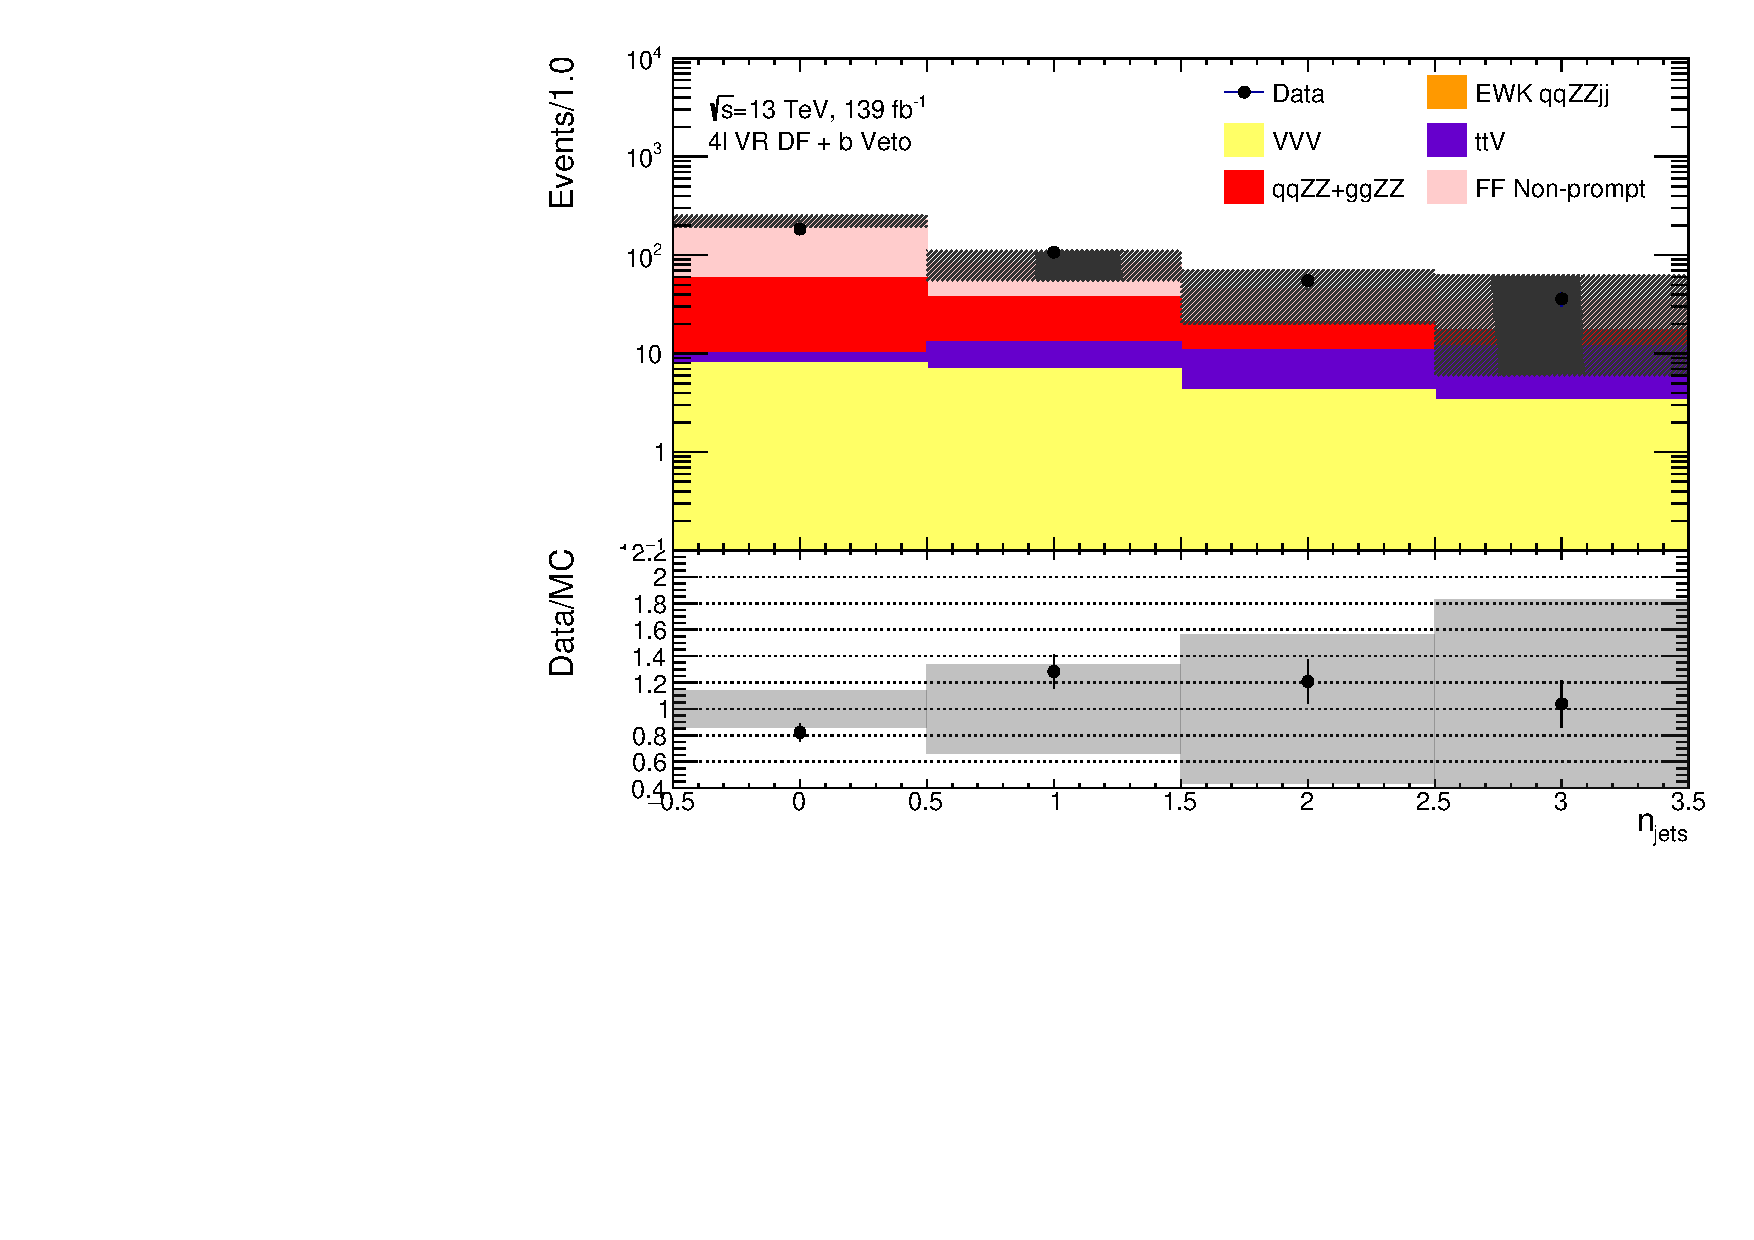
\includegraphics[width = 0.85\linewidth]{figures/Analysis/Background/Overlay_VRDF_FFApplied_n_jets.pdf}
        \caption{VRDF: $n_{jets}$ \label{fig:AllDataMCYield_VRDF_njet} }
    \end{subfigure}
    \begin{subfigure}{.48\textwidth}
        \centering
        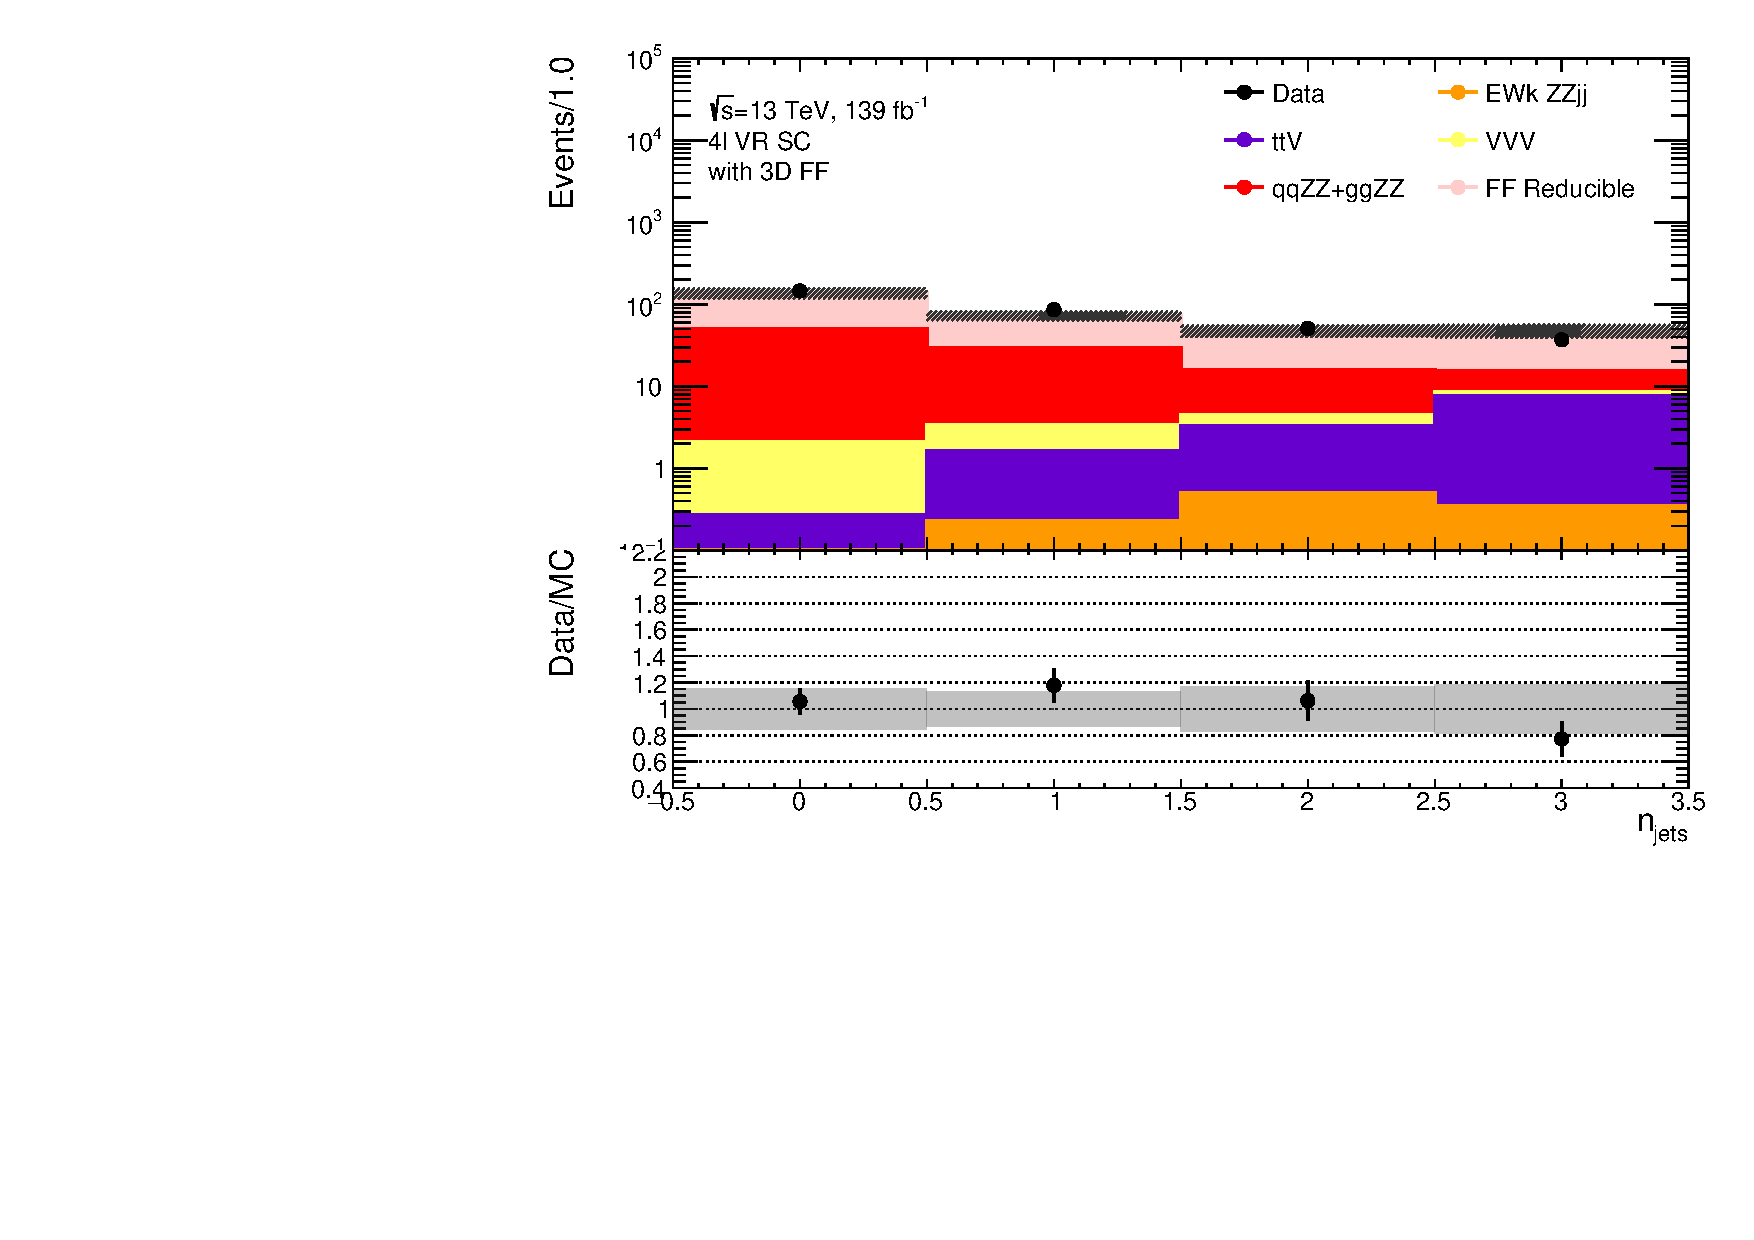
\includegraphics[width = 0.85\linewidth]{figures/Analysis/Background/Overlay_VRSC_FFApplied_n_jets.pdf}
        \caption{VRSC: $n_{jets}$ \label{fig:AllDataMCYield_VRSC_njet}}
    \end{subfigure}
        \caption{ Comparison of data to the total MC prediction and fake background in validation regions (left) as a function of three kinematic observables used to parametrize the fake efficiencies in the combined control region.\label{fig:AllDataMCYield}}
\end{figure}

\subsubsection{Signal Region Estimation}
\label{subsubsec:SREstimation}
Similar to the validation regions, the background in the signal region is estimated by applying the fake factor to the baseline-anti-signal leptons in the not-signal quadruplets, as discussed in Section \ref{subsubsec:EstimationStrategy}. Distributions in Figure \ref{fig:MCFFRedComparison} compare the fake background predicted from MC and estimated from the fake-factor method in the VBS-Enhanced region as a function of $\mFourL$. The data-driven estimate of the fake background is in close agreement with that predicted by the MC.

\begin{figure}[htb]
    \centering
    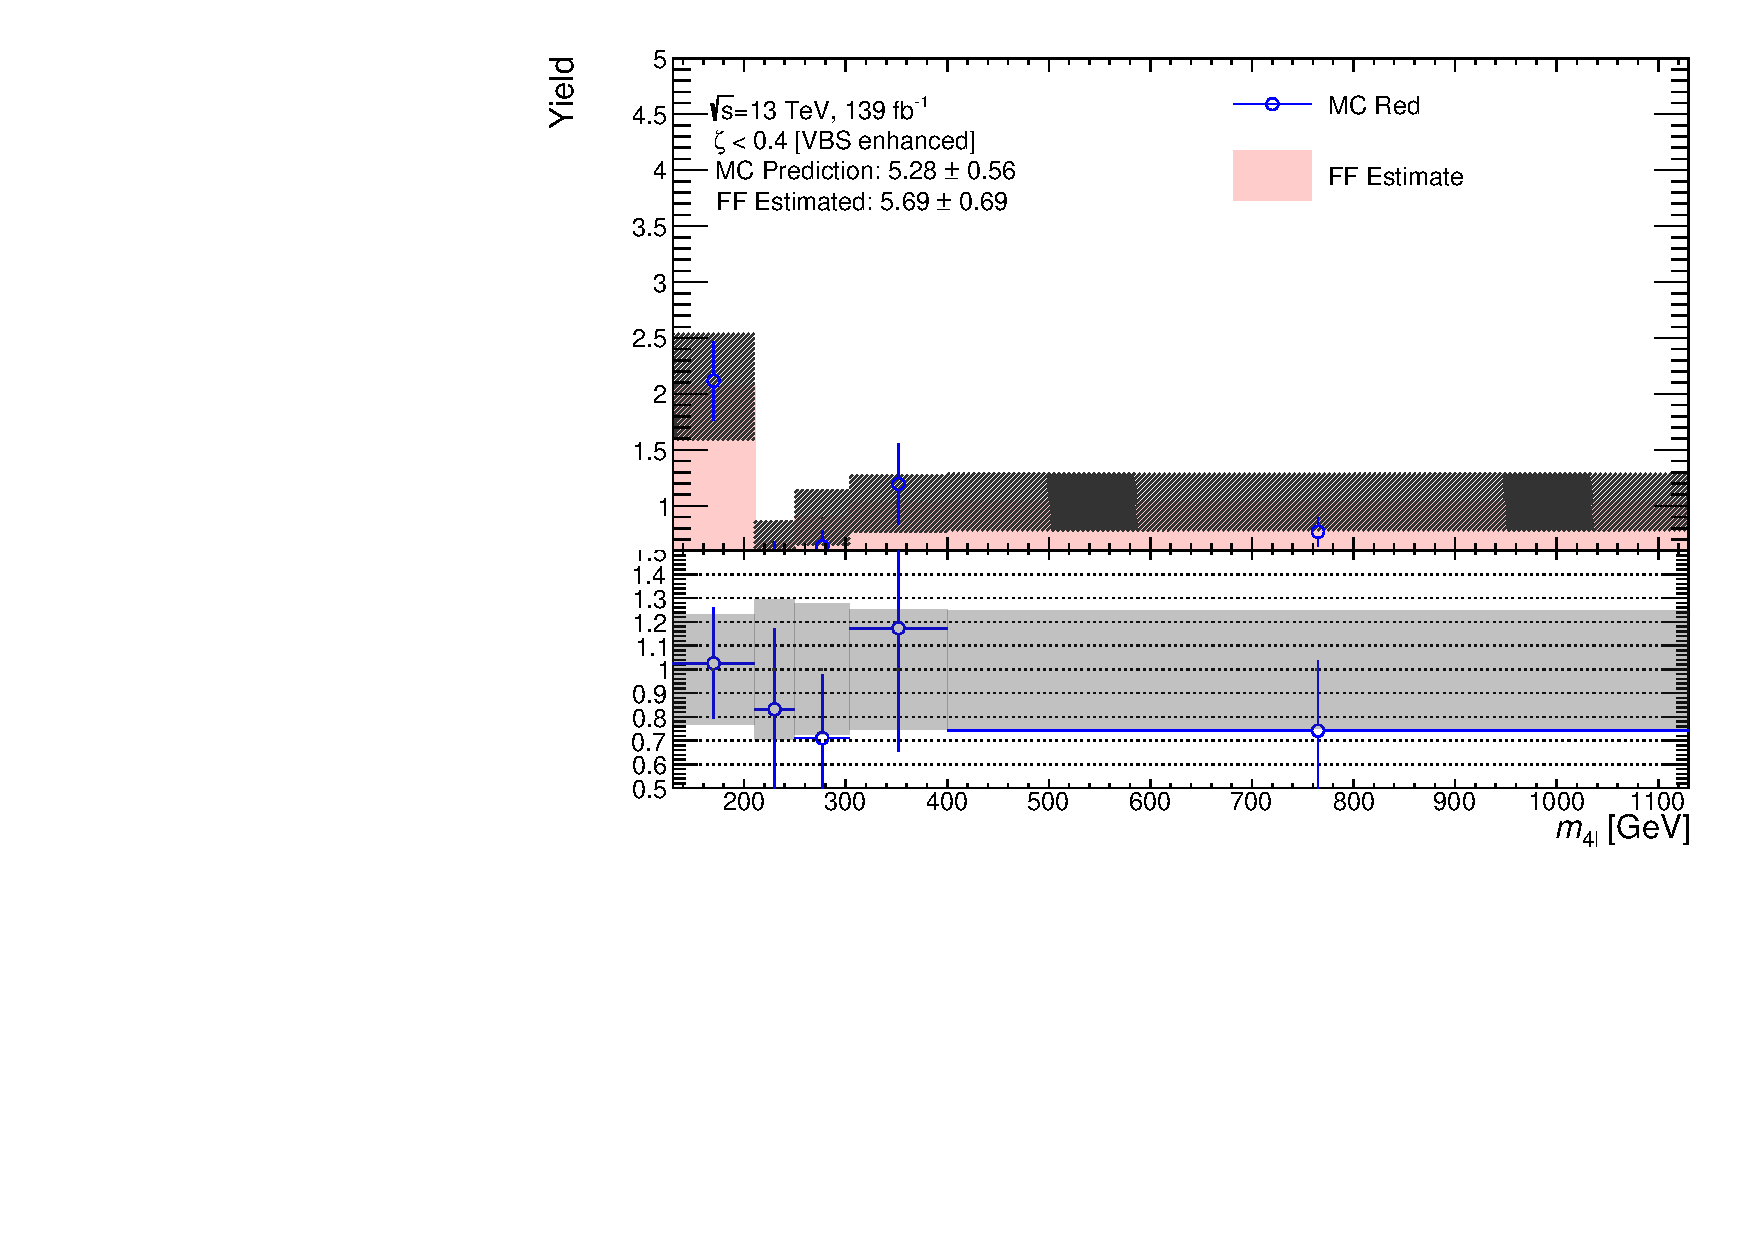
\includegraphics[width=0.5\textwidth]{figures/Analysis/Background/MCRedCompare_VBS_Enhanced_M4l.pdf}
    \caption{ MC prediction and fake-factor method estimate of the fake background as a function of $\mFourL$ in the VBS-Enhanced region. Black bands represent the systematic uncertainties from the fake factor method. \label{fig:MCFFRedComparison}}
\end{figure}

Figure \ref{fig:MCFFRedStack} shows the total SM detector-level predictions and estimated fake background as a function of $\mFourL$ and $p_{T,4\ell}$ in the VBS-Enhanced region. The signal MC predictions include the combination of EWK $qqZZjj$ and QCD parton and gluon-loop initiated $qqZZ$ $ggZZ$ samples, respectively. The FF Non-Prompt, $ttV$, and $VVV$ distributions show the three background processes, where FF ~Non-Prompt is estimated using the data-driven fake factor method. The ratio panels show the predicted high values of signal-to-background ratios. 

\begin{figure}[htb]
    \centering
    \includegraphics[width=0.48\textwidth]{figures/Analysis/Background/RedStack_VBSEnhanced_M4l.pdf}
    \includegraphics[width=0.48\textwidth]{figures/Analysis/Background/RedStack_VBSEnhanced_Pt4l.pdf}
    \caption{ Detector level SM predictions of signal and background processes along with the fake background estimated from the fake-factor method as a function of $\mFourL$(left) and $\ptFourL$ (right) in the VBS-Enhanced region. \label{fig:MCFFRedStack} }
\end{figure}